\documentclass[12pt,]{article}
\usepackage{lmodern}
\usepackage{amssymb,amsmath}
\usepackage{ifxetex,ifluatex}
\usepackage{fixltx2e} % provides \textsubscript
\ifnum 0\ifxetex 1\fi\ifluatex 1\fi=0 % if pdftex
  \usepackage[T1]{fontenc}
  \usepackage[utf8]{inputenc}
\else % if luatex or xelatex
  \ifxetex
    \usepackage{mathspec}
  \else
    \usepackage{fontspec}
  \fi
  \defaultfontfeatures{Ligatures=TeX,Scale=MatchLowercase}
\fi
% use upquote if available, for straight quotes in verbatim environments
\IfFileExists{upquote.sty}{\usepackage{upquote}}{}
% use microtype if available
\IfFileExists{microtype.sty}{%
\usepackage{microtype}
\UseMicrotypeSet[protrusion]{basicmath} % disable protrusion for tt fonts
}{}
\usepackage[margin = 1.2in]{geometry}
\usepackage{hyperref}
\PassOptionsToPackage{usenames,dvipsnames}{color} % color is loaded by hyperref
\hypersetup{unicode=true,
            colorlinks=true,
            linkcolor=red,
            citecolor=blue,
            urlcolor=red,
            breaklinks=true}
\urlstyle{same}  % don't use monospace font for urls
\usepackage{color}
\usepackage{fancyvrb}
\newcommand{\VerbBar}{|}
\newcommand{\VERB}{\Verb[commandchars=\\\{\}]}
\DefineVerbatimEnvironment{Highlighting}{Verbatim}{commandchars=\\\{\}}
% Add ',fontsize=\small' for more characters per line
\newenvironment{Shaded}{}{}
\newcommand{\KeywordTok}[1]{\textcolor[rgb]{0.00,0.00,1.00}{#1}}
\newcommand{\DataTypeTok}[1]{#1}
\newcommand{\DecValTok}[1]{#1}
\newcommand{\BaseNTok}[1]{#1}
\newcommand{\FloatTok}[1]{#1}
\newcommand{\ConstantTok}[1]{#1}
\newcommand{\CharTok}[1]{\textcolor[rgb]{0.00,0.50,0.50}{#1}}
\newcommand{\SpecialCharTok}[1]{\textcolor[rgb]{0.00,0.50,0.50}{#1}}
\newcommand{\StringTok}[1]{\textcolor[rgb]{0.00,0.50,0.50}{#1}}
\newcommand{\VerbatimStringTok}[1]{\textcolor[rgb]{0.00,0.50,0.50}{#1}}
\newcommand{\SpecialStringTok}[1]{\textcolor[rgb]{0.00,0.50,0.50}{#1}}
\newcommand{\ImportTok}[1]{#1}
\newcommand{\CommentTok}[1]{\textcolor[rgb]{0.00,0.50,0.00}{#1}}
\newcommand{\DocumentationTok}[1]{\textcolor[rgb]{0.00,0.50,0.00}{#1}}
\newcommand{\AnnotationTok}[1]{\textcolor[rgb]{0.00,0.50,0.00}{#1}}
\newcommand{\CommentVarTok}[1]{\textcolor[rgb]{0.00,0.50,0.00}{#1}}
\newcommand{\OtherTok}[1]{\textcolor[rgb]{1.00,0.25,0.00}{#1}}
\newcommand{\FunctionTok}[1]{#1}
\newcommand{\VariableTok}[1]{#1}
\newcommand{\ControlFlowTok}[1]{\textcolor[rgb]{0.00,0.00,1.00}{#1}}
\newcommand{\OperatorTok}[1]{#1}
\newcommand{\BuiltInTok}[1]{#1}
\newcommand{\ExtensionTok}[1]{#1}
\newcommand{\PreprocessorTok}[1]{\textcolor[rgb]{1.00,0.25,0.00}{#1}}
\newcommand{\AttributeTok}[1]{#1}
\newcommand{\RegionMarkerTok}[1]{#1}
\newcommand{\InformationTok}[1]{\textcolor[rgb]{0.00,0.50,0.00}{#1}}
\newcommand{\WarningTok}[1]{\textcolor[rgb]{0.00,0.50,0.00}{\textbf{#1}}}
\newcommand{\AlertTok}[1]{\textcolor[rgb]{1.00,0.00,0.00}{#1}}
\newcommand{\ErrorTok}[1]{\textcolor[rgb]{1.00,0.00,0.00}{\textbf{#1}}}
\newcommand{\NormalTok}[1]{#1}
\usepackage{graphicx,grffile}
\makeatletter
\def\maxwidth{\ifdim\Gin@nat@width>\linewidth\linewidth\else\Gin@nat@width\fi}
\def\maxheight{\ifdim\Gin@nat@height>\textheight\textheight\else\Gin@nat@height\fi}
\makeatother
% Scale images if necessary, so that they will not overflow the page
% margins by default, and it is still possible to overwrite the defaults
% using explicit options in \includegraphics[width, height, ...]{}
\setkeys{Gin}{width=\maxwidth,height=\maxheight,keepaspectratio}
\setlength{\emergencystretch}{3em}  % prevent overfull lines
\providecommand{\tightlist}{%
  \setlength{\itemsep}{0pt}\setlength{\parskip}{0pt}}
\setcounter{secnumdepth}{5}
% Redefines (sub)paragraphs to behave more like sections
\ifx\paragraph\undefined\else
\let\oldparagraph\paragraph
\renewcommand{\paragraph}[1]{\oldparagraph{#1}\mbox{}}
\fi
\ifx\subparagraph\undefined\else
\let\oldsubparagraph\subparagraph
\renewcommand{\subparagraph}[1]{\oldsubparagraph{#1}\mbox{}}
\fi

%%% Use protect on footnotes to avoid problems with footnotes in titles
\let\rmarkdownfootnote\footnote%
\def\footnote{\protect\rmarkdownfootnote}

%%% Change title format to be more compact
\usepackage{titling}

% Create subtitle command for use in maketitle
\newcommand{\subtitle}[1]{
  \posttitle{
    \begin{center}\large#1\end{center}
    }
}

\setlength{\droptitle}{-2em}
  \title{}
  \pretitle{\vspace{\droptitle}}
  \posttitle{}
  \author{}
  \preauthor{}\postauthor{}
  \date{}
  \predate{}\postdate{}

\usepackage{booktabs}
\usepackage{longtable}
\usepackage{array}
\usepackage{multirow}
\usepackage[table]{xcolor}
\usepackage{wrapfig}
\usepackage{float}
\usepackage{colortbl}
\usepackage{pdflscape}
\usepackage{tabu}
\usepackage{threeparttable}
\usepackage{threeparttablex}
\usepackage[normalem]{ulem}
\usepackage{makecell}

\usepackage{placeins}
\usepackage{hyperref}
\usepackage{fancyhdr}
\usepackage{setspace}
\usepackage{chngcntr}
\onehalfspacing
\counterwithin{figure}{section}
\counterwithin{table}{section}
\usepackage{rotating}
\usepackage{dcolumn}

\begin{document}

\interfootnotelinepenalty=10000

\pagenumbering{gobble}

\begin{centering}

\begin{figure}[!h]
\centering

\includegraphics[width=5cm, height=5cm]{figures/UNamur.png}
\end{figure}

\vspace{3.5cm}

\Large
{\bf Green companies are the future:\\ Evidence from \\US publicly traded companies}

\vspace{1.5cm}

\normalsize
{\bf Pierrick KINIF}

\vspace{1cm}
\normalsize
Supervisors :\\
\vspace{0.5cm}

Prof. Sophie Béreau\\
Prof. Jean-Yves Gnabo
\vspace{1cm}

\normalsize
Thesis submitted for the Master's Degree \\
in Business Management and Administration, \\
Finance Specialization

\vspace{1cm}
\normalsize
{\bf ACADEMIC YEAR 2017 - 2018\\}
\end{centering}

\fancypagestyle{firstpage}{%
  \cfoot{\scriptsize University of Namur, ASBL\\
Faculty of Economics, Social Sciences and Business Administration - Department of Business Administration\\
Rempart de la Vierge 8, B-5000 Namur, Belgium, Phone. +32 [0]81 72 48 41/49 58, Fax +32 [0]81 72 48 40}
} \thispagestyle{firstpage} \renewcommand{\footrulewidth}{0pt}
\renewcommand{\headrulewidth}{0pt}

\newpage

\pagenumbering{roman}

\begin{centering}
\huge
\title{Green companies are the future: Evidence from US publicly traded companies}

\maketitle

\normalsize
\begin{abstract}

Providing evidence that companies with better Corporate Environmental Performance (i.e. CEP) have also better Corporate Financial Performance (i.e. CFP) have been a lively debate in the literature.  Two major opposite trends emerged. Some scholars provided evidence of a positive link between CEP and CFP while others have demonstrated a negative relationship. Using a panel data of 393 US publicly traded companies for the period 2012-2014, this study first investigates the impact of process-based CEP on outcome-based CEP. Then, it explores whether the combined effect of process-based and outcome-based CEP influences CFP and observes the time influence (i.e. short-term vs long-term) of the relationship.

Findings of this study provide evidence that process-based CEP positively influences outcome-based CEP and support the idea that it does pay to be green. More precisely, it demonstrates that both process and outcome-based CEP have a positive impact on CFP, no matter the time horizon, and is stronger with a long-term perspective than a short-term perspective. This study emphasizes strong incentives for companies to invest in environmental strategies.

\end{abstract}
\providecommand{\keywords}[1]
{
  \small    
  \textbf{\textit{Keywords---}} #1
}
\keywords{Corporate Environmental Performance, Corporate Financial Performance, Panel Data, Global Warming}
\end{centering}

\newpage

\section*{Author's Note}

This master's thesis has been written in \texttt{R\ Markdown}
(\textsc{Allaire et al.}, \protect\hyperlink{ref-Allaire2016}{2016}) to
make it transparent and reproducible for the reader. All resources are
available on my GitHub account
\texttt{https://github.com/pkinif/Thesis}. The latter is organized
following the methodology of \textsc{Gandrud}
(\protect\hyperlink{ref-Gandrud2013b}{2013}). Each section of this
thesis corresponds to an \texttt{R\ Markdown} file in the \texttt{Child}
folder. The \texttt{Child/ThesisSkeleton.Rmd} file is the
\texttt{parent} document which merges all the \texttt{child} directories
into a consolidated pdf document, namely the one you are reading. The
\texttt{Child/Analysis} sub-folder contains a list of makefiles whose
outputs are saved into \texttt{Child/Analysis/DataBase}.

The platform I have used is \texttt{Rstudio} which is an open source
software for \texttt{R}. Here are the information of my session :

\begin{Shaded}
\begin{Highlighting}[]
\KeywordTok{sessionInfo}\NormalTok{()}
\end{Highlighting}
\end{Shaded}

\begin{verbatim}
## R version 3.4.4 (2018-03-15)
## Platform: x86_64-w64-mingw32/x64 (64-bit)
## Running under: Windows 10 x64 (build 16299)
## 
## Matrix products: default
## 
## locale:
## [1] LC_COLLATE=French_Belgium.1252  LC_CTYPE=French_Belgium.1252   
## [3] LC_MONETARY=French_Belgium.1252 LC_NUMERIC=C                   
## [5] LC_TIME=French_Belgium.1252    
## 
## attached base packages:
## [1] stats     graphics  grDevices utils     datasets  methods   base     
## 
## other attached packages:
##  [1] kableExtra_0.9.0           knitr_1.20                
##  [3] plyr_1.8.4                 RCurl_1.95-4.10           
##  [5] bitops_1.0-6               rlist_0.4.6.1             
##  [7] rvest_0.3.2                xml2_1.2.0                
##  [9] xtable_1.8-2               ggpubr_0.1.6              
## [11] magrittr_1.5               car_2.1-6                 
## [13] tidyquant_0.5.4            forcats_0.3.0             
## [15] stringr_1.3.0              readr_1.1.1               
## [17] tidyr_0.8.0                tidyverse_1.2.1           
## [19] quantmod_0.4-12            TTR_0.23-3                
## [21] lubridate_1.7.2            tibble_1.4.2              
## [23] PerformanceAnalytics_1.5.2 xts_0.10-2                
## [25] zoo_1.8-1                  purrr_0.2.4               
## [27] Hmisc_4.1-1                ggplot2_2.2.1             
## [29] survival_2.41-3            lattice_0.20-35           
## [31] stargazer_5.2.1            data.table_1.10.4-3       
## [33] dplyr_0.7.4                plm_1.6-6                 
## [35] Formula_1.2-2             
## 
## loaded via a namespace (and not attached):
##  [1] nlme_3.1-131.1      pbkrtest_0.4-7      RColorBrewer_1.1-2 
##  [4] httr_1.3.1          rprojroot_1.3-2     tools_3.4.4        
##  [7] backports_1.1.2     R6_2.2.2            rpart_4.1-13       
## [10] lazyeval_0.2.1      mgcv_1.8-23         colorspace_1.3-2   
## [13] nnet_7.3-12         gridExtra_2.3       mnormt_1.5-5       
## [16] curl_3.1            compiler_3.4.4      quantreg_5.35      
## [19] cli_1.0.0           formatR_1.5         htmlTable_1.11.2   
## [22] SparseM_1.77        sandwich_2.4-0      scales_0.5.0       
## [25] checkmate_1.8.5     lmtest_0.9-35       psych_1.7.8        
## [28] quadprog_1.5-5      digest_0.6.15       foreign_0.8-69     
## [31] minqa_1.2.4         rmarkdown_1.9       base64enc_0.1-3    
## [34] pkgconfig_2.0.1     htmltools_0.3.6     lme4_1.1-15        
## [37] htmlwidgets_1.0     rlang_0.2.0         readxl_1.0.0       
## [40] rstudioapi_0.7      bindr_0.1.1         jsonlite_1.5       
## [43] acepack_1.4.1       Matrix_1.2-12       Rcpp_0.12.16       
## [46] Quandl_2.8.0        munsell_0.4.3       stringi_1.1.7      
## [49] yaml_2.1.18         MASS_7.3-49         grid_3.4.4         
## [52] parallel_3.4.4      bdsmatrix_1.3-3     crayon_1.3.4       
## [55] haven_1.1.1         splines_3.4.4       hms_0.4.2          
## [58] pillar_1.2.1        reshape2_1.4.3      glue_1.2.0         
## [61] evaluate_0.10.1     latticeExtra_0.6-28 modelr_0.1.1       
## [64] nloptr_1.0.4        MatrixModels_0.4-1  miscTools_0.6-22   
## [67] cellranger_1.1.0    gtable_0.2.0        assertthat_0.2.0   
## [70] broom_0.4.3         viridisLite_0.3.0   bindrcpp_0.2       
## [73] cluster_2.0.6       maxLik_1.3-4
\end{verbatim}

\vspace{3cm}

\section*{Author's Declaration}

I certify that this master's thesis does not incorporate without
acknowledegment, any material previously submitted for a degree or
diploma in any university; and that to the best of my knowledge and
belief, it does not contain any material previously published or written
by another person where due reference is not made in the text.

\vspace*{3cm}

\noindent\hrulefill\hrulefill\hrulefill\hfill\hrulefill\hrulefill

\noindent\small\textsc{signed}\hfill\textsc{dated}

\newpage

\begin{acknowledgements}
\addchaptertocentry{\acknowledgementname} 
I would first like to express my deep gratitude to Professor Sophie Béreau and Professor Jean-Yves Gnabo, my research supervisors, for their guidance and useful critiques. I would also like to thank Professor Paulo Roberto Feldmann and Professor Paulo Tromboni de Souza Nascimento who taught me the necessary scientific research expertise to fulfill this master's thesis. I am also very thankful to Mr. Patrick Virakam, Risk reporting team leader at Banque International à Luxembourg, who gave me the computer skills I needed to carry out this research project. The developer and blogging community, notably in the field of Reproducible Research, has also been incredibly important. I wish finally to thank my family and friends for their support and encouragement.\ldots
\end{acknowledgements}

\newpage

\renewcommand{\contentsname}{Table of Contents}

\setcounter{tocdepth}{3} \tableofcontents

\newpage

\addcontentsline{toc}{section}{List of Tables}

\listoftables
\addcontentsline{toc}{section}{List of Figures} \listoffigures

\newpage

\section*{List of Abbreviations}\label{list-of-abbreviations}
\addcontentsline{toc}{section}{List of Abbreviations}

\vspace{2cm}

\begin{table}[H]
\centering
\begin{tabular}{ll}
\toprule
Abbreviation & Term\\
\midrule
A & Audit Score\\
BPLM & Breusch-Pagan Lagrange Multiplier\\
CaP & Carbon Productivity\\
CEP & Corporate Environmental Performance\\
CFP & Corporate Financial Performance\\
\addlinespace
CSP & Corporate Social Performance\\
EDV & Environmental Disclosure Variables\\
EMV & Environmental Management Measures\\
EPV & Environmental Performance Variables\\
ESG & Environmental, Social and Governmental\\
\addlinespace
FE & Fixed Effetcs\\
GICS & Global Industry Classification Standard\\
ISO & The International Organization for Standardization\\
KPI & Key Performance Indicator\\
OLS & Ordinary Least Square\\
\addlinespace
ppm & Parts Per Million\\
RE & Random Effetcs\\
ROA & Return on Asset\\
ROE & Return on Equity\\
SPL & Sustainability Pay Link\\
\addlinespace
SRI & Socially Responsible Investments\\
STC & Sustainability Themed Committee\\
VIF & Variance Inflation Factor\\
WastP & Waste Productivity\\
WatP & Water Productivity\\
\bottomrule
\end{tabular}
\end{table}

\newpage

\pagenumbering{arabic}

\pagestyle{fancy} \renewcommand{\headrulewidth}{0.4pt}
\renewcommand{\footrulewidth}{0pt} \fancyhead[CO,CE]{Introduction}

\section*{Introduction}\label{introduction}
\addcontentsline{toc}{section}{Introduction}

Over the past decades, humanity was progressively becoming aware of the
finiteness of earth's resources and its impact on the current global
warming. The club of Rome, with their book \emph{``The limits to
growth''}, concluded that \emph{``if the present growth trends in world
population, industrialization, pollution, food production, resource
depletion continue unchanged, the limits to growth on this planet will
be reached sometime within the next one hundred years''}
(\textsc{Meadows et al.}, \protect\hyperlink{ref-Meadows1972}{1972}:
p23). In the nineties, \textsc{Houghton and Change}
(\protect\hyperlink{ref-HoughtonClimateChange19951996}{1996}) have also
pleaded that \emph{``in the absence of mitigation policies, greenhouse
gas emissions will continue to rise during the next century''} (p9).
This will \emph{``increase the global mean surface air temperature
relative to 1990 of about 2°C by 2100\ldots{}leading to harsh climatic
repercussions''} (p23).

Over the last 30 years, these predictions have started to come true. For
the first time in 400 000 years, atmospheric carbon dioxide crossed, in
1950, the level of 300 parts per
million\footnote{A concentration of 300 ppm means that for every million air particles, 300 of them are carbon dioxide molecules, namely a carbon concentration of 0.03\%.}
(i.e.~ppm) (\textsc{Petit et al.},
\protect\hyperlink{ref-Petit1999}{1999}; \textsc{Pieter Tans et al.},
\protect\hyperlink{ref-PieterTans2018}{2018}). According to the NOAA's
Annual Greenhouse Gas Index, the atmospheric abundance of \(CO_{2}\) has
increased by an average of 1.80 ppm per year from 1979 to 2016
(\textsc{Butler and Montzka}, \protect\hyperlink{ref-Butler2016}{2016}).
In May 2018, the global level of carbon dioxide has reached 410 ppm
(\textsc{Pieter Tans et al.},
\protect\hyperlink{ref-PieterTans2018}{2018}). This increase led to
direct effects.

Since the last 19th century, the average temperature of the planet
increased by 1.1 degrees Celsius. Most of the warming occurred in the
past 35 years, with 16 of the 17 warmest years on record occurring since
2001 (\textsc{Gistemp Team},
\protect\hyperlink{ref-GistempTeam2018}{2018}; \textsc{Hansen et al.},
\protect\hyperlink{ref-Hansen2010}{2010}). Data from NASA's Gravity
Recovery and Climate Experiment show Greenland lost 150 to 250 cubic
kilometers of ice per year between 2002 and 2006, while Antarctica lost
about 152 cubic kilometers of ice between 2002 and 2005 (\textsc{Gistemp
Team}, \protect\hyperlink{ref-GistempTeam2018}{2018}). \textsc{Church
and White} (\protect\hyperlink{ref-Church2006}{2006}) has shown that, in
the last century, the global sea level rose about 8 inches. Due to a
high carbon dioxide absorption level (\textsc{Sabine et al.},
\protect\hyperlink{ref-Sabine2004}{2004}), the acidity of surface ocean
waters has increased by about 30 percent (\textsc{NOAA's Pacific Marine
Environmental Laboratory}, n.d.) leading, \emph{inter alia}, to harsh
repercussions to corals.

Ecosystem degradation and resources depletion engender a threat to
firm's longevity (\textsc{Dowell et al.},
\protect\hyperlink{ref-Dowell2000}{2000}). In his speech at Lloyds of
London 2015, Mark Carney, Governor of the Bank of England and Chair of
the Financial Stability Board, identified climate change as one of the
most material threats to financial stability (\textsc{Elliott},
\protect\hyperlink{ref-Elliott2015}{2015}). The \textsc{Business and
Sustainable Development Commission}
(\protect\hyperlink{ref-BusinessandSustainableDevelopmentCommission2017}{2017})
(p12) report stated: \emph{``\ldots{} businesses need to pursue social
and environmental sustainability as avidly as they pursue market share
and shareholder value\ldots{} If they don't, the costs and uncertainty
of unsustainable development could swell until there is no viable world
in which to do business.''} In other words, adopting environmental
strategies ensure companies' competitiveness and survival in the near
future.

\textsc{Testa et al.} (\protect\hyperlink{ref-Testa2018}{2018}) have
shown that, due to institutional pressure or the influence of
stakeholders, a majority of companies have integrated, either
substantially or symbolically (i.e.~greenwashing), proactive
environmental practices. However, according to \textsc{Scarpellini et
al.}
(\protect\hyperlink{ref-Scarpellinieconomicfinanceinterface2016}{2016}),
green projects are still not common in companies of many countries
because of significant barriers and a negligible culture of excluding
sustainable development from an organization's strategy.

People's actions reflect a variable mix of altruistic motivation,
material self-interest, and social or self-image concerns
(\textsc{Bénabou and Tirole},
\protect\hyperlink{ref-BenabouIncentivesProsocialBehavior2006}{2006}).
Hence, for more than 40 years, scholars have analyzed the Corporate
Environmental Performance (i.e.~CEP) and Corporate Financial Performance
(i.e.~CFP) nexus to provide evidence that it does pay to be green and to
convince companies to incorporate environmental sustainability into
their core values and strategies (\textsc{Lu et al.},
\protect\hyperlink{ref-Ludecadedebatenexus2014}{2014}).

The International Organization for Standardization (\textsc{ISO},
\protect\hyperlink{ref-ISO2013}{2013}) defines CEP as \emph{``measurable
results of an organization's management of its environmental aspects''}.
The CFP construct assesses the outcomes of business strategy
(\textsc{Bansal and DesJardine},
\protect\hyperlink{ref-Bansal2014}{2014}) and is a primary, fundamental
indicator of organizational performance and long-term survival of an
organization (\textsc{Hamann et al.},
\protect\hyperlink{ref-Hamann2013}{2013}).

The relationship between CEP and CFP has been broadly discussed in the
literature and led to inconsistent empirical findings (\textsc{Endrikat
et al.},
\protect\hyperlink{ref-EndrikatMakingsenseconflicting2014}{2014}). Two
major opposite trends emerged. Some scholars (\textsc{Delmas et al.},
\protect\hyperlink{ref-Delmas2015}{2015}; \textsc{Miroshnychenko et
al.},
\protect\hyperlink{ref-MiroshnychenkoGreenpracticesfinancial2017}{2017})
provided evidence of a positive link between CEP and CFP while others
(\textsc{Busch and Hoffmann}, \protect\hyperlink{ref-Busch2011a}{2011};
\textsc{Fernando et al.}, \protect\hyperlink{ref-Fernando2010}{2010})
have demonstrated a negative relationship. This inconclusiveness may
come from the multidimensionality of both focal constructs
(\textsc{Albertini}, \protect\hyperlink{ref-Albertini2013}{2013};
\textsc{Endrikat et al.},
\protect\hyperlink{ref-EndrikatMakingsenseconflicting2014}{2014};
\textsc{Griffin and Mahon}, \protect\hyperlink{ref-Griffin1997}{1997})
given that commonly shared understanding or conceptualization of CEP and
CFP has not been established so far (\textsc{Etzion},
\protect\hyperlink{ref-Etzion2007}{2007}; \textsc{Hamann et al.},
\protect\hyperlink{ref-Hamann2013}{2013}).

Indeed, \textsc{Endrikat et al.}
(\protect\hyperlink{ref-EndrikatMakingsenseconflicting2014}{2014}) argue
that a two-group classification of CEP can be deduced from the
literature. (i) Process-based CEP which refers to \emph{``a strategic
level and focuses on managerial principles and processes such as
environmental objectives, environmental policies, or environmental
management structures''}. (ii) Outcome-based CEP which reflects
\emph{``the observable and quantifiable results of these efforts
(\textsc{Delmas et al.}, \protect\hyperlink{ref-Delmas2011a}{2011}) and
refers to measures such as the number of released pollutants or the
ratio of recycled waste to total waste''}.

Regarding CFP, scholars have adopted three broad subdivisions:
market-based (i.e.~investor returns), accounting-based (i.e.~accounting
returns), and perceptual (i.e.~survey) measures (\textsc{Lu et al.},
\protect\hyperlink{ref-Ludecadedebatenexus2014}{2014}). Furthermore, the
multidimensionality of CFP includes a wide array of estimations that may
capture a firm's ability to generate value in the short-term and
company's future growth prospects assessed by the external stakeholders
(\textsc{Opler and Titman}, \protect\hyperlink{ref-Opler1994}{1994}).

\textsc{Endrikat et al.}
(\protect\hyperlink{ref-EndrikatMakingsenseconflicting2014}{2014}) have
highlighted the need for a better understanding of the
multidimensionality of both CEP and CFP constructs. Furthermore,
\textsc{King and Lenox} (\protect\hyperlink{ref-King2002}{2002})
suggested that \emph{``When does it pay to be green?''} may be a more
important question than \emph{``Does it pay to be green?''}.
\textsc{Griffin and Mahon} (\protect\hyperlink{ref-Griffin1997}{1997})
were the first to call for studies that look at the CEP-CFP relationship
over time. \textsc{Busch and Friede}
(\protect\hyperlink{ref-Busch2018}{2018}) demonstrated that, at a
meta-research level, evidence of a time dependency on the CEP-CFP link
are not significant and that the call of \textsc{Griffin and Mahon}
(\protect\hyperlink{ref-Griffin1997}{1997}) remains, to date,
unanswered. Therefore, using a panel data of 393 US publicly traded
companies for the period 2012-2014, this study first investigates the
impact of process-based CEP on outcome-based CEP. Then, it explores
whether the combined effect of process-based and outcome-based CEP
influences CFP and observes the time influence (i.e.~short-term vs
long-term) of the relationship.

The rest of the paper is organized as follows: the next section reviews
the literature regarding the CEP-CFP nexus. Then, I describe my database
and methodology. Next, the results are presented and discussed. Finally,
I summarize the main contributions to the literature and highlight
potential future research.

\FloatBarrier
\newpage
\fancyhead[CO,CE]{Literature Review}

\section{Literature Review}\label{literature-review}

\subsection{CFP as a broad
meta-construct}\label{cfp-as-a-broad-meta-construct}

CFP is a broad meta-construct and scholars have adopted three broad
subdivisions: market-based, accounting-based, and perceptual measures
(\textsc{Orlitzky et al.}, \protect\hyperlink{ref-Orlitzky2003}{2003}).

\emph{Market-based measures} (e.g.~price-earning ratio or Tobin's Q)
consider that returns should be measured from the perspective of the
shareholders (\textsc{Cochran and Wood},
\protect\hyperlink{ref-Cochran1984a}{1984}). They incorporate intangible
assets and reputational effects (\textsc{Busch and Hoffmann},
\protect\hyperlink{ref-Busch2011a}{2011}) and can be highly influenced
by speculations, rumors and capital market breakdowns (\textsc{Wright},
\protect\hyperlink{ref-Wright2004}{2004}).

\emph{Accounting-based measures} require profitability and asset
utilization indicators such as Return on Asset (i.e.~ROA) or Return on
Equity (i.e.~ROE) (\textsc{Cochran and Wood},
\protect\hyperlink{ref-Cochran1984a}{1984}; \textsc{Wu},
\protect\hyperlink{ref-Wu2006}{2006}). These indicators capture a firm's
internal efficiency (\textsc{Cochran and Wood},
\protect\hyperlink{ref-Cochran1984a}{1984}). Indeed, \textsc{Orlitzky et
al.} (\protect\hyperlink{ref-Orlitzky2003}{2003}) highlight that
\emph{``accounting returns are subject to managers' discretionary
allocations of funds to different projects and policy choices, and thus
reflect internal decision-making capabilities and managerial performance
rather than external market responses to organizational (non-market)
actions''}. Accounting-based indicators are highly influenced by the
industrial sector characteristics (\textsc{Montgomery and Wernerfelt},
\protect\hyperlink{ref-Montgomery1988}{1988}).

\emph{Perceptual measures} of CFP is a more subjective approach
(\textsc{Lu et al.},
\protect\hyperlink{ref-Ludecadedebatenexus2014}{2014}) based on external
(e.g.~Fortune magazine rankings) and internal (e.g.~Management surveys)
perceptual metrics (\textsc{Peloza},
\protect\hyperlink{ref-Peloza2009}{2009}). These indicators ask survey
respondents to provide subjective estimates of, for instance, the firm's
\emph{``soundness of financial position''}, \emph{``wise use of
corporate assets''}, or \emph{``financial goal achievement relative to
competitors''} (\textsc{Orlitzky et al.},
\protect\hyperlink{ref-Orlitzky2003}{2003}).

Based on a recent critical review, \textsc{Lu et al.}
(\protect\hyperlink{ref-Ludecadedebatenexus2014}{2014}) have shown that,
of the three types of CFP measures, accounting-based ones are the most
frequency used, followed by the market-based measures, and perceptual
measures. Scholars also tend to alleviate weaknesses of one type of
indicators by the use of another (\textsc{McWilliams et al.},
\protect\hyperlink{ref-McWilliams2006}{2006}). For instance,
\textsc{King and Lenox} (\protect\hyperlink{ref-King2002}{2002}) and
\textsc{Delmas et al.} (\protect\hyperlink{ref-Delmas2015}{2015}) have
used ROA and Tobin's Q as proxies for approaching CFP. \textsc{Menguc
and Ozanne} (\protect\hyperlink{ref-Menguc2005}{2005}) considered market
share, sales growth and profit after tax. \textsc{Husted and Allen}
(\protect\hyperlink{ref-Husted2007}{2007}) used management surveys while
\textsc{Verschoor} (\protect\hyperlink{ref-Verschoor1999}{1999}) adopted
the Fortune magazine rankings.

\subsection{CEP as a broad
meta-construct}\label{cep-as-a-broad-meta-construct}

CEP is also a broad meta-constructs and no common definition exist in
the literature (\textsc{Albertini},
\protect\hyperlink{ref-Albertini2013}{2013}; \textsc{Endrikat et al.},
\protect\hyperlink{ref-EndrikatMakingsenseconflicting2014}{2014}).
Scholars have used a wide variety of indicators as proxies for
approaching the green performance of companies. \textsc{Albertini}
(\protect\hyperlink{ref-Albertini2013}{2013}) use a three-group
classification to summarize CEP measures : (i) \emph{Environmental
Management Measures} (i.e.~EMV) which mostly refer to environmental
strategy, integration of environmental issues into strategic planning
processes, environmental practices, process-driven initiatives,
product-driven management systems, ISO 14001 certification,
environmental management system adoption, and participation in voluntary
programs (\textsc{Molina-Azorín et al.},
\protect\hyperlink{ref-Molina-Azorin2009}{2009}; \textsc{Schultze and
Trommer}, \protect\hyperlink{ref-Schultze2012}{2012}). (ii)
\emph{Environmental Performance Variables} (i.e.~EPV) which are mostly
measures quantified in physical units (carbon dioxide emissions,
physical waste, water consumption, toxic release) that can be positive
(emission reduction) or negative (emission generated)
(\textsc{Albertini}, \protect\hyperlink{ref-Albertini2013}{2013}). (iii)
\emph{Environmental Disclosure Variables} (i.e.~EDV) such as information
releases regarding toxic emission (\textsc{Hamilton},
\protect\hyperlink{ref-Hamilton1995}{1995}), environmental awards
(\textsc{Chen et al.},
\protect\hyperlink{ref-Chencrosscountrycomparisongreen2018}{2018}),
environmental accidents and crises (\textsc{Blacconiere and Patten},
\protect\hyperlink{ref-Blacconiere1994}{1994}), and environmental
investment announcements (\textsc{Gilley et al.},
\protect\hyperlink{ref-Gilley2000}{2000}).

\textsc{Endrikat et al.}
(\protect\hyperlink{ref-EndrikatMakingsenseconflicting2014}{2014}) split
up CEP into two sub-dimension. On the one hand, \emph{process-based CEP}
which can be linked to the EMV approach of \textsc{Albertini}
(\protect\hyperlink{ref-Albertini2013}{2013}). It refers to \emph{``a
strategic level and focuses on managerial principles and processes such
as environmental objectives, environmental policies, or environmental
management structures''}. On the other hand, \emph{outcome-based CEP}
which can be linked to the EPV dimension of \textsc{Albertini}
(\protect\hyperlink{ref-Albertini2013}{2013}). It reflects \emph{``the
observable and quantifiable results of these efforts (\textsc{Delmas et
al.}, \protect\hyperlink{ref-Delmas2011a}{2011}) and refers to measures
such as the number of released pollutants or the ratio of recycled waste
to total waste''}. According to \textsc{Xie and Hayase}
(\protect\hyperlink{ref-Xie2007}{2007}), process-based CEP can be
considered as a preliminary step of outcome-based CEP. Besides, scholars
demonstrated that the first approach has a positive impact on the second
one which in turn has a positive impact on financial performance
(\textsc{Chen et al.},
\protect\hyperlink{ref-Chencrosscountrycomparisongreen2018}{2018};
\textsc{Li et al.}, \protect\hyperlink{ref-Li2017}{2017}).

CEP can also be linked to the Environmental, Social and Governmental
(i.e.~ESG) framework or also called, Socially Responsible Investments
(i.e.~SRI). ESG investing provides criteria that allow investors and
advisors to select investments that align with their values as well as
their financial goals (\textsc{Fulton et al.},
\protect\hyperlink{ref-Fulton2012}{2012}). It applies a set of
investment screens to select or exclude assets based on ESG criteria
(\textsc{Renneboog et al.},
\protect\hyperlink{ref-Renneboog2008}{2008}). A plethora of
organizations have developed methodologies to attribute an ESG score to
companies and support investors who consider corporate governance
insights into their investment processes. For instance, Sustainalytics,
based in New York and Thomson Reuters with the Asset4 ESG database.
Scholars (\textsc{Halbritter and Dorfleitner},
\protect\hyperlink{ref-Halbritter2015}{2015}; \textsc{Miroshnychenko et
al.},
\protect\hyperlink{ref-MiroshnychenkoGreenpracticesfinancial2017}{2017})
have used these ESG scores as proxies for CEP.

\subsection{Two perspectives on CEP}\label{two-perspectives-on-cep}

\textsc{Friedman} (\protect\hyperlink{ref-MiltonFriedman1970}{1970})
considers investment in pollution efficient technology as a deviation
from the profit maximization goal (i.e.~an increase in cost). According
to him, \emph{``businessmen who want to promote desirably social
ends\ldots{}are unwitting puppets of the intellectual forces that have
been undermining the basis of a free society''}. In recent decades, this
paradigm has been widely challenged. The literature is showing growing
evidence that improving a company's environmental performance can lead
to better economic or financial performance.

\textsc{Ambec and Lanoie} (\protect\hyperlink{ref-Ambec2008}{2008})
demonstrated that the expenses incurred to reduce pollution can be
partly or completely offset by gains made elsewhere. \textsc{Porter and
van der Linde} (\protect\hyperlink{ref-Porter1995}{1995}) argued that
properly crafted environmental standards can trigger innovation offsets,
allowing companies to improve their resource productivity. He redefined
the self-concept of value creation. According to him, companies have to
create shared value. Sharing value creation involves building economic
value which addresses the current needs and challenges of the society
(\textsc{Porter et al.}, \protect\hyperlink{ref-Porter2011a}{2011};
\textsc{Porter and Kramer}, \protect\hyperlink{ref-Porter2011}{2011}).
In the same logic, \textsc{Freeman}
(\protect\hyperlink{ref-Freeman1984}{1984}) calls for a radical
rethinking of our firm's model. He argues that companies have to
consider their stakeholders (i.e.~any group or individual who can affect
or is affected by the achievement of an organization's objectives (p25))
or otherwise face a negative contest from non-shareholder groups
(e.g.~boycotts, lawsuits, and protests). In other words,
\textsc{Freeman} (\protect\hyperlink{ref-Freeman1984}{1984}) summarizes
the idea that companies should consider corporate environmental
performance as an undeniable cost of doing business.

\subsection{Does it pay to be green?}\label{does-it-pay-to-be-green}

More and more companies are developing profitable business strategies
that deliver tangible social benefits (\textsc{Testa et al.},
\protect\hyperlink{ref-Testa2018}{2018}) and that embrace the new
business paradigm of \textsc{Freeman}
(\protect\hyperlink{ref-Freeman1984}{1984}), \textsc{Porter and van der
Linde} (\protect\hyperlink{ref-Porter1995}{1995}) and \textsc{Ambec and
Lanoie} (\protect\hyperlink{ref-Ambec2008}{2008}). However, others
prefer keeping the old fashion way of \textsc{Friedman}
(\protect\hyperlink{ref-MiltonFriedman1970}{1970}). This dichotomy has
interested scholars and since they have sought to empirically answer the
question, \emph{``Does it pay to be green?''}. As claimed by \textsc{Lu
et al.} (\protect\hyperlink{ref-Ludecadedebatenexus2014}{2014}), in a
competitive business world, answering this question is crucial to
provide a genuine economic justification to the new paradigm.

The relationship between CEP and CFP has been broadly discussed in the
literature and led to inconsistent empirical findings (\textsc{Endrikat
et al.},
\protect\hyperlink{ref-EndrikatMakingsenseconflicting2014}{2014}). Two
major opposite trends emerged. Some scholars provided evidence of a
positive link between CEP and CFP while others have demonstrated a
negative relationship.

\textsc{Delmas et al.} (\protect\hyperlink{ref-Delmas2015}{2015}) found
that improving CEP causes a decline in ROA while an increase in Tobin's
q. Unlike \textsc{Cavaco and Crifo}
(\protect\hyperlink{ref-Cavaco2014}{2014}) and \textsc{Muhammad et al.}
(\protect\hyperlink{ref-Muhammadrelationshipenvironmentalperformance2015}{2015}),
who obtained a positive relation between ROA and CEP while no relation
between Tobin's Q and CEP. Results of \textsc{Miroshnychenko et al.}
(\protect\hyperlink{ref-MiroshnychenkoGreenpracticesfinancial2017}{2017})
show that internal green practices (i.e.~pollution prevention and green
supply chain management) are the major environmental drivers of
financial performance, while external green practices (i.e.~green
product development) play a secondary role in determining financial
performance. Besides, according to them, the adoption of ISO 14001
appears to have a negative impact on financial performance.
\textsc{Fernando et al.} (\protect\hyperlink{ref-Fernando2010}{2010})
observed that all else equal, toxic firms can realize a higher valuation
by becoming environmentally neutral but they found no such financial
benefit to neutral firms becoming green. \textsc{Busch and Hoffmann}
(\protect\hyperlink{ref-Busch2011a}{2011}) found that process-based CEP
(in terms of carbon management) negatively affects CFP, while
outcome-based CEP (in terms of carbon emissions) has a positive
influence on CFP. \textsc{Song et al.}
(\protect\hyperlink{ref-SongCanenvironmentalmanagement2017}{2017})
provided evidence that environmental management is significantly
positively related to financial performance in the following year while
no significant in the current year. \textsc{Fisher-Vanden and Thorburn}
(\protect\hyperlink{ref-Fisher-Vanden2008}{2008}) found that companies
announcing membership in environmental programs experience significantly
negative abnormal stock returns. Results of \textsc{Przychodzen and
Przychodzen}
(\protect\hyperlink{ref-PrzychodzenRelationshipsecoinnovationfinancial2015}{2015})
indicate that companies involved in environmental innovation process
were generally characterized by higher ROA and ROE and lower earnings
retention ratio.

Some scholars advanced that the multidimensionality of CEP and CFP
constructs is one reason why the conclusion of the relationship has been
so mixed (\textsc{Albertini},
\protect\hyperlink{ref-Albertini2013}{2013}; \textsc{Endrikat et al.},
\protect\hyperlink{ref-EndrikatMakingsenseconflicting2014}{2014}).
However, the large number of studies in the last three decades allowed
the appearance of recent
meta-analyses\footnote{Initially, the literature focused on the link between Corporate Social Performance (i.e. CSP) and Corporate Financial Performance. Orlitzky and Benjamin (2001) were the first to consider CEP as apart from CSP. Given that Busch and Friede (2018) could not detect statistically significant differences between the effects of environmental CEP and social-related CSP on CFP and concludes that good CSP pays off, whether social or environmental related, this study considers CSP equals to CEP.}
(\textsc{Albertini}, \protect\hyperlink{ref-Albertini2013}{2013};
\textsc{Busch and Friede}, \protect\hyperlink{ref-Busch2018}{2018};
\textsc{Dixon-Fowler et al.},
\protect\hyperlink{ref-Dixon-Fowler2013}{2013}; \textsc{Endrikat et
al.}, \protect\hyperlink{ref-EndrikatMakingsenseconflicting2014}{2014};
\textsc{Lu et al.},
\protect\hyperlink{ref-Ludecadedebatenexus2014}{2014}; \textsc{Orlitzky
and Benjamin}, \protect\hyperlink{ref-Orlitzky2001}{2001};
\textsc{Orlitzky et al.}, \protect\hyperlink{ref-Orlitzky2003}{2003};
\textsc{Wang et al.},
\protect\hyperlink{ref-WangMetaAnalyticReviewCorporate2016}{2016};
\textsc{Wu}, \protect\hyperlink{ref-Wu2006}{2006}) and all confirm that
indeed it does pay to be green. More precisely, a positive and
bidirectional relationship does exist between CEP and CFP meaning that
successful firms may have the resources necessary to improve their
environmental performance, which in turn increases financial benefits
that can be invested back into further improvements of CEP
(\textsc{Endrikat et al.},
\protect\hyperlink{ref-EndrikatMakingsenseconflicting2014}{2014}).

\subsection{When does it pay to be
green?}\label{when-does-it-pay-to-be-green}

\textsc{Griffin and Mahon} (\protect\hyperlink{ref-Griffin1997}{1997})
were the first to call for studies that look at the CEP-CFP relation
over time. While scholars has been mainly answering the question:
\emph{``Does it pay to be green?''} some have recently tried to move
forward and gained interest in answering the call of \textsc{Griffin and
Mahon} (\protect\hyperlink{ref-Griffin1997}{1997}) with the following
question: \emph{``When does it pay to be green?''} (\textsc{Manrique and
Martí-Ballester},
\protect\hyperlink{ref-ManriqueAnalyzingEffectCorporate2017}{2017}).

\textsc{Zhang and Chen} (\protect\hyperlink{ref-Zhang2017}{2017}) have
shown that CEP has a negative relationship with short-term financial
performance and a positive relationship with long-term CFP.
\textsc{Delmas et al.} (\protect\hyperlink{ref-Delmas2015}{2015})
observed that the more a company decreases carbon emissions, the more
positive the investors' perceptions of future market performance, and
the lower its short-term financial performance. \textsc{Song et al.}
(\protect\hyperlink{ref-SongCanenvironmentalmanagement2017}{2017}) have
shown that corporate environmental management has a significant positive
correlation with future financial performance while no significant
correlation with current financial performance. \textsc{Manrique and
Martí-Ballester}
(\protect\hyperlink{ref-ManriqueAnalyzingEffectCorporate2017}{2017})
demonstrated that in times of economic crisis, firms which improve their
corporate environmental performance improve their corporate financial
performance, this effect being weaker for firms in developed countries,
where only the short-term corporate financial performance improves than
for firms in emerging and developing countries, where the short and
long-term corporate financial performance improve. \textsc{Chen et al.}
(\protect\hyperlink{ref-Chencrosscountrycomparisongreen2018}{2018}) have
shown that a firms green performance not only impact an organization's
financial performance in that particular year but also impact the year
that follows.

Those empirical results provide pieces of evidence that no common
consensus have been found yet to answer the question: \emph{``When does
it pay to be green?''}. To that extent, \textsc{Busch and Friede}
(\protect\hyperlink{ref-Busch2018}{2018}) demonstrated that at a
meta-research level, the evidence of a time dependency on the CEP-CFP
link is not significant and that the call of \textsc{Griffin and Mahon}
(\protect\hyperlink{ref-Griffin1997}{1997}) remains to date unanswered.

To capture the time dimension in the CFP-CEP nexus, scholars consider
accounting-based measures as a proxy for short-term CFP and market-based
measures as a proxy for long-term CFP (\textsc{Delmas et al.},
\protect\hyperlink{ref-Delmas2015}{2015}; \textsc{Endrikat et al.},
\protect\hyperlink{ref-EndrikatMakingsenseconflicting2014}{2014};
\textsc{Manrique and Martí-Ballester},
\protect\hyperlink{ref-ManriqueAnalyzingEffectCorporate2017}{2017};
\textsc{Miroshnychenko et al.},
\protect\hyperlink{ref-MiroshnychenkoGreenpracticesfinancial2017}{2017};
\textsc{Zhang and Chen}, \protect\hyperlink{ref-Zhang2017}{2017}).
Indeed, \textsc{Endrikat et al.}
(\protect\hyperlink{ref-EndrikatMakingsenseconflicting2014}{2014})
highlight that on the one hand, accounting-based measures capture
immediate impacts but do not seize long-term effects, unlike
market-based measures which integrate estimations of a firm's future
prospects and reflect the notion of external stakeholders.

Taking into account previous theoretical arguments and considering
varying empirical findings with regards to the CEP-CFP nexus, this study
hypothesizes the following :

\vspace{0.5cm} \textbf{Hypothesis 1.} Process-based CEP have a positive
impact on Outcome-based CEP

\textbf{Hypothesis 2.} Outcome-based CEP have a positive impact on
short-term CFP

\textbf{Hypothesis 3.} Outcome-based CEP have a positive impact on
long-term CFP

\textbf{Hypothesis 4.} Process-based CEP have a positive impact on
short-term CFP

\textbf{Hypothesis 5.} Process-based CEP have a positive impact on
long-term CFP

\vspace{0.5cm}

The research framework of this study, inspired by \textsc{Li Suhong et
al.} (\protect\hyperlink{ref-LiSuhong2017}{2017}) and \textsc{Chen et
al.}
(\protect\hyperlink{ref-Chencrosscountrycomparisongreen2018}{2018}), is
summarized in figure \ref{ResearchFramework}.

\vspace{3cm}

\begin{figure}[!h]
\centering
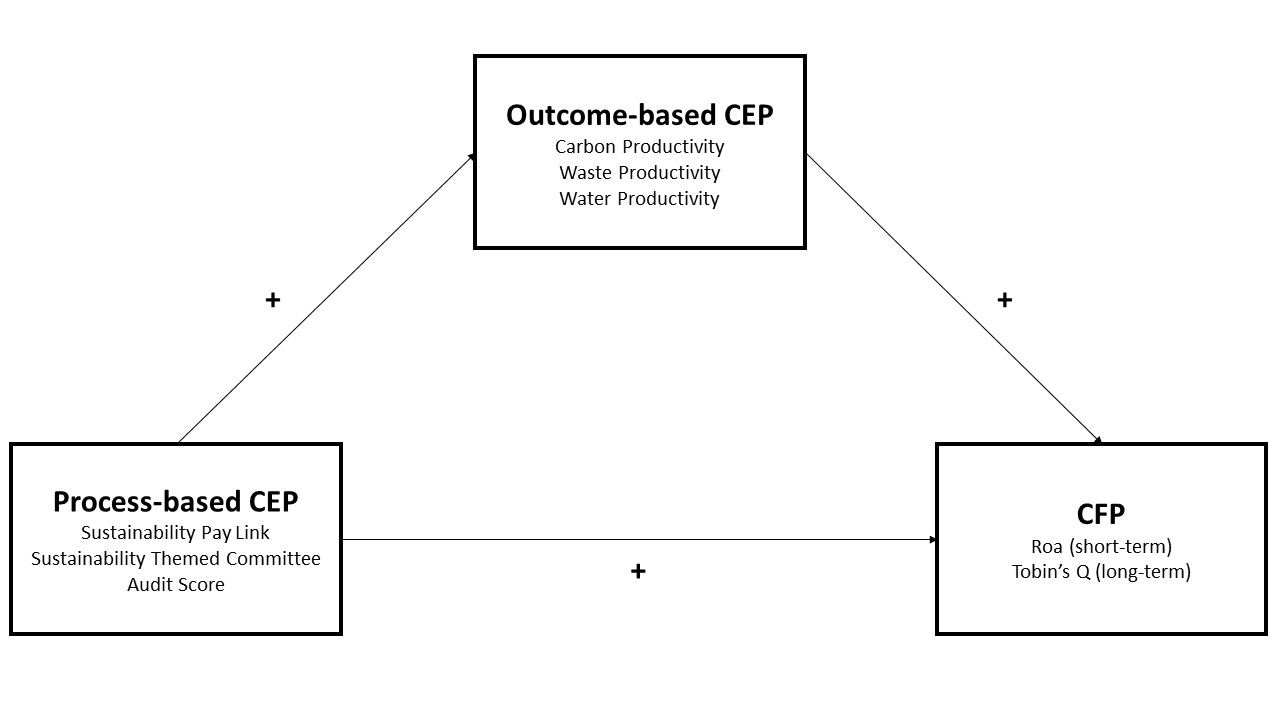
\includegraphics[width=14cm, height=12cm]{figures/ResearchFramework.jpg}
\caption{Research Framework}
\label{ResearchFramework}
\end{figure}

\FloatBarrier
\newpage
\fancyhead[CO,CE]{Data Description}

\section{Data Description}\label{data-description}

\subsection{Overview}\label{overview}

The starting point of the data collection was the Newsweek Green
Ranking. This ranking had assessed the world's largest publicly-traded
companies in the US and in the world since 2009. It has been developed
through a collaboration between Newsweek, Corporate Knights Capital, HIP
Investor Inc and leading sustainability minds from nongovernmental
organizations and the academic and accounting communities.

The ranking attributes an overall green score to companies. This score
is based on a weighted average of key performance indicators (KPI's).
This study uses these KPI's to approach both process-based and
outcome-based CEP of the 500 largest publicly-traded companies in the
United States. As a result of making a transition to a 100\% rules-based
approach, the methodology for the 2014 Newsweek Green Rankings differs
considerably from the framework used in the 2012 Newsweek Green
Rankings. Therefore, this study considers only
\href{http://www.newsweek.com/green/worlds-greenest-companies-2014}{\texttt{2014}},
\href{http://www.newsweek.com/green-2015/top-green-companies-world-2015}{\texttt{2015}}
and
\href{http://www.newsweek.com/green-2016/top-green-companies-world-2016}{\texttt{2016}}
ranking. Among those three ranking and of the 500 US companies, 405
companies were listed for each year.

Even though green rankings were published in 2014, 2015 and 2016, each
company is evaluated based on 2012, 2013 and 2014 company data.
Therefore, measures for Corporate Financial Performance will be based on
2012, 2013 and 2014 fundamental data. Financial data have been collected
on
\href{http://www.morningstar.be/be/default.aspx}{\texttt{Morningstar}},
\href{http://www.stockpup.com/}{\texttt{Stockpup}} and
\href{https://ycharts.com/}{\texttt{Ycharts}} using
\href{https://cran.r-project.org/}{\texttt{R}} technology. The data
collection process is described in
\emph{``\protect\hyperlink{appendix-a-database-construction}{Appendix A:
Database construction}''}. Of the 405 initial companies, a total of 12
were dropped because of missing data. The final sample includes 393
publicly-traded companies in the US covering the period from 2012 till
2014 inclusively.

\autoref{VarDef} gives an overview of variables of the econometric
model. Following sections deeply explain each variable.

\begin{table}[h]
\centering
\caption{Variables Description} 
\label{VarDef}
\begin{tabular}{lp{3cm}p{10cm}}
  \hline
\hline
 & Variables & Description \\ 
  \hline
1 & ROA & Earnings before interest over total firm assets \\ 
  2 & Tobin's Q & The ratio of a firm’s market value to the replacement cost of its assets \\ 
  3 & CaP & Revenue (USD) / Total Greenhouse gas Emissions (CO2) \\ 
  4 & WaP & Revenue (USD) / Total water (m3) \\ 
  5 & WastP & Revenue (USD) / [Total waste generated (metric tonnes)–waste recycled/reused (tones)] \\ 
  6 & SPL & A mechanism to link the remuneration of any member of a company's senior executive team with the achievement of environmental performance targets. Dummy variable which equals 1 if such a link exists and 0 otherwise \\ 
  7 & STC & Refers to the existence of a committee at the Board of Directors level whose mandate is related to the sustainability of the company, including but not limited to environmental matters. Dummy variable which equals 1 if such a committee exists and 0 otherwise \\ 
  8 & A & Refers to the case where a company provides evidence that the latest reported environmental metrics were audited by a third party. Dummy variable which equals 1 if such evidence exist and 0 otherwise \\ 
  9 & Leverage & The ratio of long-term debt to common shareholders' equity (shareholders equity minus preferred equity) \\ 
  10 & Growth & Net margin, namely the ratio of earnings to revenue \\ 
  11 & Firm Size & Natural logarithm of total assets \\ 
  12 & Industry & Global Industry Classification Standard (GICS) of the firm. The variable takes a value from 1 to 10 where 1 = Consumer Discretionary, 2 = Consumer Staples, 3 = Energy, 4 = Financials, 5 = Health Care, 6 = Industrials, 7 = Information Technology, 8 = Materials, 9 = Pharmaceuticals / Biotechnology, 10 = Telecommunication Services and 11 = Utilities \\ 
   \hline
\end{tabular}
\end{table}

\subsection{Dependent Variables}\label{dependent-variables}

Regarding dependent variables, \textsc{Endrikat et al.}
(\protect\hyperlink{ref-EndrikatMakingsenseconflicting2014}{2014}) claim
that accounting-based measures (e.g.~Return On Asset, Return On Equity,
Return on Sales) capture immediate impacts and can be used as a proxy to
measure short-term CFP while market-based measures (e.g.~Tobin's Q,
market capitalization, market to book value) integrate estimations of a
firm's future prospects and can be better used as a proxy for long-term
CFP. Among scholars which used both measures simultaneously, ROA and
Tobin's Q are the most frequent (\textsc{Cavaco and Crifo},
\protect\hyperlink{ref-Cavaco2014}{2014}; \textsc{Delmas et al.},
\protect\hyperlink{ref-Delmas2015}{2015}; \textsc{Lioui and Sharma},
\protect\hyperlink{ref-Lioui2012}{2012}; \textsc{Manrique and
Martí-Ballester},
\protect\hyperlink{ref-ManriqueAnalyzingEffectCorporate2017}{2017};
\textsc{Muhammad et al.},
\protect\hyperlink{ref-Muhammadrelationshipenvironmentalperformance2015}{2015};
\textsc{Semenova and Hassel},
\protect\hyperlink{ref-Semenova2016}{2016}). Therefore, this study uses
ROA and Tobin's Q as a proxy for both short and long-term CFP.

\emph{ROA} is a standard accounting measure of financial performance,
which is calculated by dividing earnings before interest by total firm
assets. ROA gives information about how a company can transform assets
into profit.

\emph{Tobin's Q} is defined as the ratio of the market value of a firm
to the replacement cost of its assets (\textsc{Chung and Pruitt},
\protect\hyperlink{ref-Chung1994}{1994}). Broadly speaking, firms
displaying Tobin's Q greater than one are judged as using scarce
resources effectively and those with Tobin's Q less than one as using
resources poorly (\textsc{Lewellen and Badrinath},
\protect\hyperlink{ref-Lewellen1997}{1997}). In other words, investors
prefer companies with Tobin's Q superior to one. Due to the complexity
of calculating the replacement cost of a firm, the literature has seen
several attempts to approximate Tobin's Q (\textsc{Perfect and Wiles},
\protect\hyperlink{ref-Perfect1994}{1994}). This study collected Tobin's
Q data directly on Ycharts. The latter uses the simple approximation of
\textsc{Chung and Pruitt} (\protect\hyperlink{ref-Chung1994}{1994})
which is summarized in equation \ref{Chung}. Due to a high right-skew
(i.e.~skewness = 2.51), I use a natural logarithm transformation to
normalize the distribution of Tobin's Q (\textsc{Honaker et al.},
\protect\hyperlink{ref-Honaker2011a}{2011}).

\begin{equation}
Tobin's Q = \frac{MVE + PS + DEBT}{TA}
\label{Chung}
\end{equation}

where \(MVE\) is the product of a firm's shares prices and the number of
common stock shares outstanding, \(PS\) is the liquidating value of the
firm's outstanding preferred stock, \(DEBT\) is the value of the firm's
short-term liabilities net of its short-term assets, plus the book value
of the firm's long-term debt and \(TA\) is the book value of the total
assets of the firms.

\subsection{Independent Variables}\label{independent-variables}

Both process-based and outcome-based CEP has been approached with KPI's
of the Newsweek Green Ranking. I use ``Sustainability Pay Link'',
``Sustainability Themed Committee'', and ``Audit'' as proxies for
process-based CEP and ``Carbon Productivity'', ``Water Productivity''
and ``Waste Productivity'' as proxies for outcome-based
CEP\footnote{Newsweek Green Ranking has another KPI that captures outcome-based CEP (i.e. Energy Productivity). Due to multicollinearity concern (Variance Inflation Factor superior to 5 for both Energy and Carbon Productivity),  I do not consider it into my model.}.

\emph{A Sustainability Pay Link} (i.e.~SPL) is a mechanism to link the
remuneration of any member of a company's senior executive team with the
achievement of environmental performance targets. A score of 1 accrues
to the company when such a link exists and a score of 0 otherwise.

\emph{A Sustainability Themed Committee} (i.e.~STC) refers to the
existence of a committee at the board of directors level whose mandate
is related to the sustainability of the company, including but not
limited to environmental matters. A score of 1 accrues to the company
when such a link exists and a score of 0 otherwise.

\emph{An Audit Score} (i.e.~A) refers to the case where a company
provides evidence that the latest reported environmental metrics were
audited by a third party. A score of 1 accrues to the company if such an
audit has been performed, and a score of 0 otherwise.

\emph{Carbon Productivity} (i.e.~CaP), \emph{Water Productivity}
(i.e.~WatP) and \emph{Waste Productivity} (i.e.~WastP) are calculated
through equation \ref{CaP}, \ref{WatP} and \ref{WastP}.

\begin{equation}
CaP_{it} = \frac{Revenue_{it}}{TGGE_{it}}
\label{CaP}
\end{equation}

\begin{equation}
WatP_{it} = \frac{Revenue_{it}}{TW_{it}}
\label{WatP}
\end{equation}

\begin{equation}
WastP_{it} = \frac{Revenue_{it}}{(TWG_{it} - TWRR_{it})}
\label{WastP}
\end{equation}

where \(Revenue_{it}\) is the total revenue in \(USD\), \(TGGE_{it}\) is
the total greenhouse gaz emissions in \(CO_{2}\), \(TW_{it}\) is the
total water in \(m_{3}\), \(TWG_{it}\) is the total waste generated in
metric tons and \(TWRR\) is the total waste recycled and reused in
metric tons.

\subsection{Control Variables}\label{control-variables}

Scholars have argued that misspecified models may be another reason for
the inconsistency of the empirical results in the CEP-CFP nexus
(\textsc{McWilliams et al.},
\protect\hyperlink{ref-McWilliams2006}{2006}; \textsc{Surroca et al.},
\protect\hyperlink{ref-Surroca2010}{2010}; \textsc{Telle},
\protect\hyperlink{ref-Telle2006}{2006}). To improve the construct and
to avoid the endogeneity issue due to omitted variables (\textsc{Roberts
and Whited}, \protect\hyperlink{ref-Roberts2013}{2013}),
\textsc{Endrikat et al.}
(\protect\hyperlink{ref-EndrikatMakingsenseconflicting2014}{2014}) have
highlighted potential determinants of the relationship between CEP and
CFP: firm size, industry sector, and capital structure. In a
meta-analysis study, \textsc{Lu et al.}
(\protect\hyperlink{ref-Ludecadedebatenexus2014}{2014}) argued that
growth rate is equally important. This study uses those four
determinants as control variables.

The common way to approach \emph{firm size} is to use the natural
logarithm of total assets (\textsc{Delmas et al.},
\protect\hyperlink{ref-Delmas2015}{2015}; \textsc{Miroshnychenko et
al.},
\protect\hyperlink{ref-MiroshnychenkoGreenpracticesfinancial2017}{2017}).
To approach the company \emph{industry sector}, I use the Global
Industry Classification Standard (GICS)
\footnote{The GICS classification is composed of eleven industry sectors, namely: Consumer Discretionary, Consumer Staples, Energy, Financials, Health Care, Industrials, Information Technology, Materials, Pharmaceuticals / Biotechnology, Telecommunication Services and Utilities.}.\emph{Capital
structure} is interpreted here as the financial leverage, namely as the
debt to equity ratio. The latter is measured as the ratio of long-term
debt to common shareholders' equity (shareholders equity minus preferred
equity). The \emph{growth rate} is approached through the net margin
(i.e.~the ratio of earnings to revenue).

\FloatBarrier
\newpage
\fancyhead[CO,CE]{Methodology}

\section{Methodology}\label{Methodology}

\subsection{Panel Data: a theoretical
background}\label{panel-data-a-theoretical-background}

This study uses the panel data methodology. Panel data is a common
approach to address the CFP-CEP nexus (\textsc{Albertini},
\protect\hyperlink{ref-Albertini2013}{2013}). It is considered to be one
of the most efficient analytical methods for data analysis
(\textsc{Dimitrios Asteriou},
\protect\hyperlink{ref-DimitriosAsteriou2006}{2006}). It usually
contains more degrees of freedom, less collinearity among the variables,
more efficiency and more sample variability than one-dimensional method
(i.e.cross-sectional data and time series data) giving a more accurate
inference of the parameters estimated in the model (\textsc{Hsiao},
\protect\hyperlink{ref-Hsiao2007}{2007}). \textsc{Roberts and Whited}
(\protect\hyperlink{ref-Roberts2013}{2013}) also argued that using panel
data offers a partial solution to the problem of omitted variables in
the econometric model, namely the most common causes of endogeneity in
empirical corporate finance. Panel data takes the following econometric
form :

\begin{equation}
\centering
Y_{it} = \alpha + \beta X_{it} + u_{it} 
\label{PanelData}
\end{equation}

Panel data, also called longitudinal data, includes observations on
\(i = 1,..., N\) cross- section units (e.g.~firms) over \(t = 1,..., T\)
time-periods (\textsc{Hsiao}, \protect\hyperlink{ref-Hsiao2007}{2007}).
Here, \(Y_{it}\) is the dependent variable, \(X_{it}\) represents a
\(K\)-dimensional row vectors of independent variables, \(\alpha\) is
the intercept, \(\beta\) is a \(K\)-dimensional column vectors of
parameters and \(u_{it}\) is the random disturbance term of mean equals
zero. The latter can be decomposed as
\(u_{it} = \mu_{i} + \epsilon_{it}\). The first term, \(\mu_{i}\),
represents the individual error component and is time-invariant. It can
be considered as the unobserved effect model. The second term,
\(\epsilon_{it}\), is the idiosyncratic error which is assumed
well-behaved and independent of \(X_{it}\) and \(\mu_{i}\).

The starting point of all panel data is to determine if \(\mu_{i}\) is
correlated with \(X_{it}\). In presence of correlation, then \(\mu_{i}\)
is considered as the \emph{Fixed Effect} (i.e.~FE) and the initial
equation \ref{PanelData} becomes equation \ref{Fixed}. Otherwise,
\(\mu_{i}\) is considered as the \emph{Random Effect} (i.e.~RE) and the
equation \ref{PanelData} becomes equation \ref{Random}.

\begin{equation}
\centering
Y_{it} = (\alpha + \mu{i}) + \beta X_{it} + \epsilon_{it} 
\label{Fixed}
\end{equation}

\begin{equation}
\centering
Y_{it} = \alpha + \beta X_{it} + (\epsilon_{it} + \mu{i})
\label{Random}
\end{equation}

Fixed (i.e. \autoref{Fixed}) and Random (i.e. \autoref{Random}) Effect
model imply that the Ordinary Least Square (i.e.~OLS) estimators of
\(\beta\) are inconsistent. Five assumptions are required to produce
consistent estimators with OLS : (i) a random sample of observations on
\(y\) and \((x_{1},..., x_{n})\), (ii) a random sample of \(n\)
observations, (iii) no linear relationship among the explanatory
variables, (iv) an error term that is uncorrelated with each explanatory
variables and (v) an error term with zero mean conditional on the
explanatory variables. FE Model violates the fourth assumption while RE
model implies that the common error component over individuals induces
correlation across the composite error terms making the third assumption
violated (\textsc{Croissant and Millo},
\protect\hyperlink{ref-Croissant2008}{2008}).

The R package \emph{plm} provides pertinent estimation methods to
estimate panel data model. (i) \emph{The pooled OLS estimation} ignores
the panel structure of the data and applies the same coefficient to each
individual (\textsc{Schmidheiny},
\protect\hyperlink{ref-Schmidheiny2015}{2015}). (ii) \emph{The random
effects estimation} is the feasible Generalized Least Squares estimator.
(iii) \emph{The fixed effects estimation} also called \emph{within
estimation}, transforms the original equation \ref{PanelData} in
subtracting the time average from every variable, such as :

\begin{equation}
\centering
( Y_{it} - \frac{1}{T} \displaystyle\sum_{t=1}^{T} Y_{it} ) = \beta (X_{itk} - \frac{1}{T} \displaystyle\sum_{t=1}^{T} X_{it} ) + ( \epsilon_{it} - \frac{1}{T} \displaystyle\sum_{t=1}^{T} \epsilon_{it} )
\label{FixedEffectsEstimation}
\end{equation}

The presence of RE in panel data is tested using the Breusch-Pagan
Lagrange Multiplier (i.e.~BPLM) test (\textsc{Breusch and Pagan},
\protect\hyperlink{ref-Breusch1980}{1980}) which is represented by the
\emph{plmtest} function in \emph{R}. It examines if time and/or
individual specific variance components equal zero (\textsc{Park},
\protect\hyperlink{ref-Park2011}{2011}). If H0 is verified, there is no
RE in the panel data. The presence of FE is tested by an F test
(i.e.~the function \emph{pFtest} in \emph{R}). The latter tests the
individual and/or time effects based on the comparison of the within and
the pooling model (\textsc{Croissant and Millo},
\protect\hyperlink{ref-Croissant2008}{2008}). If H0 is verified, there
is no FE in the panel data.

In case of the absence of both RE and FE, namely \(\mu_{i} = 0\), pooled
OLS estimation is the most efficient estimator (\textsc{Croissant and
Millo}, \protect\hyperlink{ref-Croissant2008}{2008}). Under FE, the
random effects estimators are biased and inconsistent given that
\(\mu_{i}\) is omitted and potentially correlated with other regressors.
Therefore, the fixed effects estimation need to be used. Under RE, the
random and fixed effects estimators are unbiased and consistent.
According to \textsc{Schmidheiny}
(\protect\hyperlink{ref-Schmidheiny2015}{2015}), scholars should prefer
the RE estimator only and only if \(E[\mu_{i}, X_{i}] = 0\). This
precondition is tested by the Hausman test (\textsc{Hausman and Taylor},
\protect\hyperlink{ref-Hausman1981}{1981}). If H0 is verified, scholars
should use the RE estimator.

\subsection{Econometric Model}\label{econometric-model}

This study uses equation \ref{CEP} to study the link between
outcome-based and process-based CEP and equation \ref{EconometricModel}
to test their effects on CFP (short-term and long-term).

\begin{equation}
\centering
Y_{it} = \alpha + \beta_{1} SPL_{it} + \beta_{2} STC_{it} + \beta_{3} A_{it} + d_{t} + u_{it}
\label{CEP}
\end{equation}

where \(Y_{it}\) is a proxy of outcome-based CEP measured as carbon
productivity, water productivity and waste productivity, \(SPL_{it}\) is
a proxy for a firm's sustainability pay link, \(STC_{it}\) is a proxy
for a firm's sustainability themed commitment, \(A_{it}\) is a proxy for
a firm's audit score, \(d_{t}\) represents the time effect and
\(u_{it}\) is the error term.

\begin{equation}
\centering
\begin{aligned}
Y_{it+1} & = & \alpha + \beta_{1} SPL_{it} + \beta_{2} STC_{it} + \beta_{3} A_{it} + \beta_{4} CaP_{it} \\
&& + { }  \beta_{5} WatP_{it} + \beta_{6} WastP_{it} + Controls_{it} + d_{t} + u_{it}
\label{EconometricModel}
\end{aligned}
\end{equation}

where \(Y_{it+1}\) is a proxy of CFP measured as ROA or Tobin's Q,
\(SPL_{it}\) is a proxy for a firm's sustainability pay link,
\(STC_{it}\) is a proxy for a firm's sustainability themed commitment,
\(A_{it}\) is a proxy for a firm's audit score, \(CP_{it}\) is a proxy
for a firm's carbon productivity, \(WatP_{it}\) is a proxy for a firm's
water productivity, \(WasP_{it}\) is a proxy for a firm's waste
productivity, \(Controls_{it}\) is a vector of control variables that
includes firm size, industry sector, financial leverage and growth,
\(d_{t}\) represents the time effect and \(u_{it}\) is the error term.

\subsection{Endogeneity concern}\label{endogeneity-concern}

Endogeneity is a common issue in empirical corporate finance. It can be
defined as a correlation between the explanatory variables and the error
term in a regression, making assumption 4 and 5 of OLS rejected
(\textsc{Roberts and Whited},
\protect\hyperlink{ref-Roberts2013}{2013}). To that extent,
\textsc{Endrikat et al.}
(\protect\hyperlink{ref-EndrikatMakingsenseconflicting2014}{2014}) claim
that the leak of endogeneity control, within the CEP-CFP nexus, could
partly explain the inconsistency of the empirical results. To provide
unbiased and consistent parameters, this study have controlled for
endogeneity.

Firstly, to avoid the first source of endogeneity, namely the omission
of variables in a model, I consider the inclusion of a vector of control
variables that explain the relation between CEP and CPF (see equation
\ref{EconometricModel}).

Secondly, recent meta-analysis provided evidence of the bidirectional
causality in the CEP-CFP nexus (\textsc{Albertini},
\protect\hyperlink{ref-Albertini2013}{2013}; \textsc{Busch and Friede},
\protect\hyperlink{ref-Busch2018}{2018}; \textsc{Dixon-Fowler et al.},
\protect\hyperlink{ref-Dixon-Fowler2013}{2013}; \textsc{Endrikat et
al.}, \protect\hyperlink{ref-EndrikatMakingsenseconflicting2014}{2014};
\textsc{Lu et al.},
\protect\hyperlink{ref-Ludecadedebatenexus2014}{2014}, \textsc{Wang et
al.}
(\protect\hyperlink{ref-WangMetaAnalyticReviewCorporate2016}{2016});
\textsc{Orlitzky and Benjamin},
\protect\hyperlink{ref-Orlitzky2001}{2001}; \textsc{Orlitzky et al.},
\protect\hyperlink{ref-Orlitzky2003}{2003}; \textsc{Wu},
\protect\hyperlink{ref-Wu2006}{2006}). This could cause simultaneous
causality between the dependent and independent variables and lead to
endogeneity concern (\textsc{Biørn and Krishnakumar},
\protect\hyperlink{ref-Biorn2008}{2008}; \textsc{Roberts and Whited},
\protect\hyperlink{ref-Roberts2013}{2013}; \textsc{Sánchez-Ballesta and
García-Meca}, \protect\hyperlink{ref-Sanchez-Ballesta2007}{2007}). To
address this issue, I use a lagged instrument in lagging observations in
independent and control variables one year behind the dependent variable
(see equation \ref{EconometricModel}). This increases the confidence of
the direction of the relationship (\textsc{Delmas et al.},
\protect\hyperlink{ref-Delmas2015}{2015}; \textsc{Hart and Ahuja},
\protect\hyperlink{ref-Hart1996}{1996}; \textsc{Miroshnychenko et al.},
\protect\hyperlink{ref-MiroshnychenkoGreenpracticesfinancial2017}{2017})
and \emph{in fine} reduces the potential simultaneity bias.

Finally, both equation \ref{CEP} and \ref{EconometricModel}, depending
on the considered dependent variable, contains Fixed Effects (see
respectively sections
\emph{``\protect\hyperlink{the-impact-of-process-based-cep-on-outcome-based-cep-1}{The
impact of process-based CEP on outcome-based CEP}''} and
\emph{``\protect\hyperlink{the-impact-of-cep-on-cfp-2}{The impact of CEP
on CFP}''} for further details) and had been estimated with the fixed
effects estimation. In presence of FE, endogeneity is clearly a concern
since the explanatory variable is correlated with a component of the
error term (\textsc{Roberts and Whited},
\protect\hyperlink{ref-Roberts2013}{2013}). However, using the fixed
effects estimation implies that FE is removed as
\(( \mu_{i} - \frac{1}{T} \displaystyle\sum_{t=1}^{T} \mu_{i} ) = 0\)
(see equation \ref{FixedEffectsEstimation}), and solves this particular
endogeneity problem (\textsc{Roberts and Whited},
\protect\hyperlink{ref-Roberts2013}{2013}).

\FloatBarrier
\newpage
\fancyhead[CO,CE]{Results}

\hypertarget{results}{\section{Results}\label{results}}

The R script of this section is available in
\emph{``\protect\hyperlink{appendix-b-results---r-script}{Appendix B:
Results - R script}''}.

\subsection{Descriptive statistics}\label{descriptive-statistics}

This section provides an overview of the database.
\autoref{DescriptiveStatistics} presents the main descriptive statistics
of each variable. The sample size of ROA (i.e.~N = 1176) is superior to
the sample size of TobinsQ (i.e.~N = 1038). Compared to ROA, calculating
Tobin's Q requires a relatively high number of financial variables and
is more susceptible to missing values (\textsc{Delmas et al.},
\protect\hyperlink{ref-Delmas2015}{2015}). This creates a disparity
among the number of observations for each dependent variables.
\textsc{Delmas et al.} (\protect\hyperlink{ref-Delmas2015}{2015})
encountered the same issue and conducted an identical analysis to check
whether this introduces a sample bias. I did the same and the
\emph{p-value} of the unpaired two-sample t-test equals 0.365 meaning
that there is no significant difference between both samples.

\autoref{Matrix} contains the matrix of correlation of the database.
There are highly significant correlations between outcome-based CEP
variables (i.e.~carbon, water and waste productivity) and process-based
CEP variables (i.e.~sustainability pay link, sustainable themed
commitment and audit score) suggesting that my model could suffer from a
high degree of multicollinearity. Multicollinearity inflates the
standard errors of the coefficients making some variables statistically
insignificant when they should be significant (\textsc{Akinwande et
al.}, \protect\hyperlink{ref-Akinwande2015}{2015}). One common practice
in the literature to detect multicollinearity is the computation of the
Variance Inflation Factor (i.e.~VIF) (\textsc{Salmerón et al.},
\protect\hyperlink{ref-Salmeron2018}{2018}). VIF indicates how much the
estimated variance of the \(i_{th}\) regression coefficient is increased
above what it would be if \(R_i^2\) equaled zero (\textsc{O'brien},
\protect\hyperlink{ref-Obrien2007}{2007}). \autoref{VIF} reports VIF of
all variables. The maximum VIF is 2,477 meaning that there is no
multicollinearity in the model (\textsc{O'brien},
\protect\hyperlink{ref-Obrien2007}{2007}).

\begin{table}[b] \centering 
  \caption{Descriptive statistics} 
  \label{DescriptiveStatistics} 
\begin{tabular}{@{\extracolsep{5pt}}lccccc} 
\\[-1.8ex]\hline 
\hline \\[-1.8ex] 
Statistic & \multicolumn{1}{c}{N} & \multicolumn{1}{c}{Mean} & \multicolumn{1}{c}{St. Dev.} & \multicolumn{1}{c}{Min} & \multicolumn{1}{c}{Max} \\ 
\hline \\[-1.8ex] 
Roa & 1,176 & 0.06 & 0.07 & $-$0.62 & 0.42 \\ 
TobinsQ & 1,038 & 0.10 & 0.38 & $-$1.30 & 1.08 \\ 
Leverage & 1,130 & 1.51 & 8.02 & 0.00 & 157.90 \\ 
Growth & 1,174 & 0.12 & 0.24 & $-$2.04 & 5.96 \\ 
FirmSize & 1,172 & 10.35 & 0.60 & 8.45 & 12.51 \\ 
Industry & 1,177 & 4.59 & 2.65 & 1 & 11 \\ 
CaP & 1,177 & 0.12 & 0.18 & 0.00 & 0.97 \\ 
WaP & 1,177 & 0.09 & 0.18 & 0.00 & 0.99 \\ 
WastP & 1,177 & 0.07 & 0.17 & 0.00 & 0.97 \\ 
SPL & 1,177 & 0.49 & 0.50 & 0 & 1 \\ 
STC & 1,177 & 0.48 & 0.50 & 0 & 1 \\ 
A & 1,177 & 0.47 & 0.50 & 0 & 1 \\ 
\hline \\[-1.8ex] 
\end{tabular} 
\end{table}

\begin{sidewaystable}[h] \centering 
  \caption{Correlation Matrix} 
  \label{Matrix} 
\small 
\begin{tabular}{@{\extracolsep{2pt}} D{.}{.}{-3} D{.}{.}{-3} D{.}{.}{-3} D{.}{.}{-3} D{.}{.}{-3} D{.}{.}{-3} D{.}{.}{-3} D{.}{.}{-3} D{.}{.}{-3} D{.}{.}{-3} D{.}{.}{-3} D{.}{.}{-3} } 
\\[-1.8ex]\hline 
\hline \\[-1.8ex] 
\multicolumn{1}{c}{} & \multicolumn{1}{c}{1} & \multicolumn{1}{c}{2} & \multicolumn{1}{c}{3} & \multicolumn{1}{c}{4} & \multicolumn{1}{c}{5} & \multicolumn{1}{c}{6} & \multicolumn{1}{c}{7} & \multicolumn{1}{c}{8} & \multicolumn{1}{c}{9} & \multicolumn{1}{c}{10} & \multicolumn{1}{c}{11} \\ 
\hline \\[-1.8ex] 
\multicolumn{1}{c}{1. Roa} & \multicolumn{1}{c}{} & \multicolumn{1}{c}{} & \multicolumn{1}{c}{} & \multicolumn{1}{c}{} & \multicolumn{1}{c}{} & \multicolumn{1}{c}{} & \multicolumn{1}{c}{} & \multicolumn{1}{c}{} & \multicolumn{1}{c}{} & \multicolumn{1}{c}{} & \multicolumn{1}{c}{} \\ 
\multicolumn{1}{c}{2. TobinsQ} & \multicolumn{1}{c}{ 0.40\textasteriskcentered \textasteriskcentered \textasteriskcentered  } & \multicolumn{1}{c}{} & \multicolumn{1}{c}{} & \multicolumn{1}{c}{} & \multicolumn{1}{c}{} & \multicolumn{1}{c}{} & \multicolumn{1}{c}{} & \multicolumn{1}{c}{} & \multicolumn{1}{c}{} & \multicolumn{1}{c}{} & \multicolumn{1}{c}{} \\ 
\multicolumn{1}{c}{3. Leverage} & \multicolumn{1}{c}{-0.02    } & \multicolumn{1}{c}{ 0.03    } & \multicolumn{1}{c}{} & \multicolumn{1}{c}{} & \multicolumn{1}{c}{} & \multicolumn{1}{c}{} & \multicolumn{1}{c}{} & \multicolumn{1}{c}{} & \multicolumn{1}{c}{} & \multicolumn{1}{c}{} & \multicolumn{1}{c}{} \\ 
\multicolumn{1}{c}{4. Growth} & \multicolumn{1}{c}{ 0.19\textasteriskcentered \textasteriskcentered \textasteriskcentered  } & \multicolumn{1}{c}{-0.02    } & \multicolumn{1}{c}{-0.07\textasteriskcentered \textasteriskcentered   } & \multicolumn{1}{c}{} & \multicolumn{1}{c}{} & \multicolumn{1}{c}{} & \multicolumn{1}{c}{} & \multicolumn{1}{c}{} & \multicolumn{1}{c}{} & \multicolumn{1}{c}{} & \multicolumn{1}{c}{} \\ 
\multicolumn{1}{c}{5. FirmSize} & \multicolumn{1}{c}{-0.27\textasteriskcentered \textasteriskcentered \textasteriskcentered  } & \multicolumn{1}{c}{-0.66\textasteriskcentered \textasteriskcentered \textasteriskcentered  } & \multicolumn{1}{c}{-0.02    } & \multicolumn{1}{c}{ 0.09\textasteriskcentered \textasteriskcentered \textasteriskcentered  } & \multicolumn{1}{c}{} & \multicolumn{1}{c}{} & \multicolumn{1}{c}{} & \multicolumn{1}{c}{} & \multicolumn{1}{c}{} & \multicolumn{1}{c}{} & \multicolumn{1}{c}{} \\ 
\multicolumn{1}{c}{6. Industry} & \multicolumn{1}{c}{-0.10\textasteriskcentered \textasteriskcentered \textasteriskcentered  } & \multicolumn{1}{c}{-0.09\textasteriskcentered \textasteriskcentered \textasteriskcentered  } & \multicolumn{1}{c}{-0.05\textasteriskcentered    } & \multicolumn{1}{c}{ 0.00    } & \multicolumn{1}{c}{ 0.06\textasteriskcentered \textasteriskcentered   } & \multicolumn{1}{c}{} & \multicolumn{1}{c}{} & \multicolumn{1}{c}{} & \multicolumn{1}{c}{} & \multicolumn{1}{c}{} & \multicolumn{1}{c}{} \\ 
\multicolumn{1}{c}{7. CaP} & \multicolumn{1}{c}{ 0.09\textasteriskcentered \textasteriskcentered \textasteriskcentered  } & \multicolumn{1}{c}{ 0.02    } & \multicolumn{1}{c}{ 0.03    } & \multicolumn{1}{c}{ 0.00    } & \multicolumn{1}{c}{ 0.07\textasteriskcentered \textasteriskcentered   } & \multicolumn{1}{c}{ 0.04    } & \multicolumn{1}{c}{} & \multicolumn{1}{c}{} & \multicolumn{1}{c}{} & \multicolumn{1}{c}{} & \multicolumn{1}{c}{} \\ 
\multicolumn{1}{c}{8. WaP} & \multicolumn{1}{c}{ 0.08\textasteriskcentered \textasteriskcentered \textasteriskcentered  } & \multicolumn{1}{c}{ 0.03    } & \multicolumn{1}{c}{ 0.06\textasteriskcentered \textasteriskcentered   } & \multicolumn{1}{c}{-0.02    } & \multicolumn{1}{c}{ 0.08\textasteriskcentered \textasteriskcentered \textasteriskcentered  } & \multicolumn{1}{c}{ 0.02    } & \multicolumn{1}{c}{ 0.67\textasteriskcentered \textasteriskcentered \textasteriskcentered  } & \multicolumn{1}{c}{} & \multicolumn{1}{c}{} & \multicolumn{1}{c}{} & \multicolumn{1}{c}{} \\ 
\multicolumn{1}{c}{9. WastP} & \multicolumn{1}{c}{ 0.07\textasteriskcentered \textasteriskcentered   } & \multicolumn{1}{c}{ 0.01    } & \multicolumn{1}{c}{ 0.08\textasteriskcentered \textasteriskcentered \textasteriskcentered  } & \multicolumn{1}{c}{-0.01    } & \multicolumn{1}{c}{ 0.07\textasteriskcentered \textasteriskcentered   } & \multicolumn{1}{c}{ 0.08\textasteriskcentered \textasteriskcentered \textasteriskcentered  } & \multicolumn{1}{c}{ 0.56\textasteriskcentered \textasteriskcentered \textasteriskcentered  } & \multicolumn{1}{c}{ 0.69\textasteriskcentered \textasteriskcentered \textasteriskcentered  } & \multicolumn{1}{c}{} & \multicolumn{1}{c}{} & \multicolumn{1}{c}{} \\ 
\multicolumn{1}{c}{10. SPL} & \multicolumn{1}{c}{-0.05\textasteriskcentered    } & \multicolumn{1}{c}{-0.11\textasteriskcentered \textasteriskcentered \textasteriskcentered  } & \multicolumn{1}{c}{-0.02    } & \multicolumn{1}{c}{-0.02    } & \multicolumn{1}{c}{ 0.29\textasteriskcentered \textasteriskcentered \textasteriskcentered  } & \multicolumn{1}{c}{ 0.09\textasteriskcentered \textasteriskcentered \textasteriskcentered  } & \multicolumn{1}{c}{ 0.06\textasteriskcentered \textasteriskcentered   } & \multicolumn{1}{c}{ 0.14\textasteriskcentered \textasteriskcentered \textasteriskcentered  } & \multicolumn{1}{c}{ 0.15\textasteriskcentered \textasteriskcentered \textasteriskcentered  } & \multicolumn{1}{c}{} & \multicolumn{1}{c}{} \\ 
\multicolumn{1}{c}{11. STC} & \multicolumn{1}{c}{ 0.00    } & \multicolumn{1}{c}{-0.10\textasteriskcentered \textasteriskcentered \textasteriskcentered  } & \multicolumn{1}{c}{-0.01    } & \multicolumn{1}{c}{-0.04    } & \multicolumn{1}{c}{ 0.29\textasteriskcentered \textasteriskcentered \textasteriskcentered  } & \multicolumn{1}{c}{ 0.06\textasteriskcentered \textasteriskcentered   } & \multicolumn{1}{c}{ 0.21\textasteriskcentered \textasteriskcentered \textasteriskcentered  } & \multicolumn{1}{c}{ 0.26\textasteriskcentered \textasteriskcentered \textasteriskcentered  } & \multicolumn{1}{c}{ 0.24\textasteriskcentered \textasteriskcentered \textasteriskcentered  } & \multicolumn{1}{c}{ 0.48\textasteriskcentered \textasteriskcentered \textasteriskcentered  } & \multicolumn{1}{c}{} \\ 
\multicolumn{1}{c}{12. A} & \multicolumn{1}{c}{-0.04    } & \multicolumn{1}{c}{-0.08\textasteriskcentered \textasteriskcentered   } & \multicolumn{1}{c}{ 0.01    } & \multicolumn{1}{c}{ 0.05\textasteriskcentered    } & \multicolumn{1}{c}{ 0.26\textasteriskcentered \textasteriskcentered \textasteriskcentered  } & \multicolumn{1}{c}{ 0.04    } & \multicolumn{1}{c}{ 0.21\textasteriskcentered \textasteriskcentered \textasteriskcentered  } & \multicolumn{1}{c}{ 0.26\textasteriskcentered \textasteriskcentered \textasteriskcentered  } & \multicolumn{1}{c}{ 0.28\textasteriskcentered \textasteriskcentered \textasteriskcentered  } & \multicolumn{1}{c}{ 0.50\textasteriskcentered \textasteriskcentered \textasteriskcentered  } & \multicolumn{1}{c}{ 0.46\textasteriskcentered \textasteriskcentered \textasteriskcentered  } \\ 
\hline \\[-1.8ex] 
\multicolumn{12}{r}{Note : * p<0.1; ** p<0.05; *** p<0.01} \\ 
\end{tabular} 
\end{sidewaystable}

\begin{table}[!] \centering 
  \caption{Variance Inflation Factor} 
  \label{VIF} 
\begin{tabular}{@{\extracolsep{5pt}} D{.}{.}{-3} D{.}{.}{-3} D{.}{.}{-3} } 
\\[-1.8ex]\hline 
\hline \\[-1.8ex] 
\multicolumn{1}{c}{} & \multicolumn{1}{c}{Roa} & \multicolumn{1}{c}{Tobin's Q} \\ 
\hline \\[-1.8ex] 
\multicolumn{1}{c}{SPL} & 1.543 & 1.487 \\ 
\multicolumn{1}{c}{STC} & 1.507 & 1.475 \\ 
\multicolumn{1}{c}{A} & 1.527 & 1.514 \\ 
\multicolumn{1}{c}{CaP} & 1.862 & 1.846 \\ 
\multicolumn{1}{c}{WaP} & 2.477 & 2.425 \\ 
\multicolumn{1}{c}{WastP} & 1.966 & 2.008 \\ 
\multicolumn{1}{c}{Leverage} & 1.021 & 1.027 \\ 
\multicolumn{1}{c}{Growth} & 1.029 & 1.026 \\ 
\multicolumn{1}{c}{FirmSize} & 1.155 & 1.134 \\ 
\multicolumn{1}{c}{Industry} & 1.025 & 1.020 \\ 
\hline \\[-1.8ex] 
\end{tabular} 
\end{table}

\subsection{Outliers treatment}\label{outliers-treatment}

\textsc{Lyu} (\protect\hyperlink{ref-Lyu2015}{2015}) defines outliers as
observations in the dataset that appear to be unusual and discordant and
which could lead to inconsistent results. \textsc{Osborne and Overbay}
(\protect\hyperlink{ref-Osborne2004}{2004}) have shown that even a small
proportion of outliers can significantly affect simple analyses
(i.e.~t-tests, correlations and ANOVAs). Outliers are an issue only and
only if they are influential, namely observations whose removal causes a
different conclusion in the analysis (\textsc{Cousineau and Chartier},
\protect\hyperlink{ref-Cousineau2010}{2010}).

How to treat influential outliers is still a lively debate in the
literature (\textsc{Cousineau and Chartier},
\protect\hyperlink{ref-Cousineau2010}{2010}; @ \textsc{Orr John et al.},
\protect\hyperlink{ref-OrrJohn1991}{1991}). \textsc{Tabachnick and
Fidell} (\protect\hyperlink{ref-Tabachnick2007}{2007}) argue that the
imputation with the mean is the best method while \textsc{Cousineau and
Chartier} (\protect\hyperlink{ref-Cousineau2010}{2010}) highlight that
it tends to reduce the spread of the population, making the observed
distribution more leptokurtic, and possibly increase the likelihood of a
type-I error. \textsc{Dang et al.}
(\protect\hyperlink{ref-Dang2009}{2009}) argue that a more elaborate
technique involves replacing outliers with possible values
(e.g.~multiple imputation) while \textsc{Barnett and Lewis}
(\protect\hyperlink{ref-Barnett1994}{1994}) would prefer to remove or
winsorize them. Alternatively, \textsc{Pollet and Meij}
(\protect\hyperlink{ref-Pollet2017}{2017}) argue that inclusion or
exclusion of outliers depend on the significativity of the results.
According to them, if results are more significant without outliers,
scholars should remove them.

Following the mindset of \textsc{Pollet and Meij}
(\protect\hyperlink{ref-Pollet2017}{2017}), I removed outliers from the
database. Influential outliers had been identified based on the Cook's
distance (\textsc{Cook}, \protect\hyperlink{ref-Cook1977}{1977}) which
is a common statistical tool to assess the influence of outliers
(\textsc{Cousineau and Chartier},
\protect\hyperlink{ref-Cousineau2010}{2010}; \textsc{JP Stevens},
\protect\hyperlink{ref-JPStevens1984}{1984}; \textsc{Zuur et al.},
\protect\hyperlink{ref-Zuurprotocoldataexploration2010}{2010}). Cook's
Distance observes the difference between the regression parameters of a
given model, \(\hat{\beta}\), and what they become if the \(i_{th}\)
data point is deleted, let's say \(\hat{\beta}_{i}\). See
\emph{``\protect\hyperlink{appendix-c-outliers-treatment}{Appendix C:
Outliers treatment}''} for further details on how I proceed.

\subsection{The impact of process-based CEP on outcome-based
CEP}\label{the-impact-of-process-based-cep-on-outcome-based-cep}

\autoref{CepResults} reports the main results of the analysis of the
impact of process-based CEP (i.e.~SPL, STC and A) on outcome-based CEP
(i.e.~CaP, WatP and WastP). Given the p-value of the F test, all models
have FE making the \emph{fixed effects estimation}, the most efficient
estimator.

Except for Model (1) which indicates no significant relation between SPL
and CaP, all models show evidence of a positive and highly statistically
significant effect of process-based CEP on outcome-based CEP. Indeed,
results demonstrate that companies, which link the remuneration of any
member of a company's senior executive team with the achievement of
environmental performance targets, have a better WatP (+0.022\%) and
WastP (+0.026\%). The fact of having a sustainability committee on the
board of directors level increases the CaP (+0.054\%), WatP (+0.062\%)
and WastP (+0.042\%). Finally, companies having their latest reported
environmental metrics audited by a third party have a higher CaP
(+0.062\%), WatP (+0.07\%) and WastP (+0.072\%). Hence, hypothesis 1 is
verified.

\begin{table}[!] \centering 
  \caption{The impact of process-based on outcome-based CEP} 
  \label{CepResults} 
\begin{tabular}{@{\extracolsep{5pt}}lccc} 
\\[-1.8ex]\hline 
\hline \\[-1.8ex] 
 & \multicolumn{3}{c}{\textit{Dependent variable:}} \\ 
\cline{2-4} 
\\[-1.8ex] & CaP & WaP & WastP \\ 
 & Model (1) & Model (2) & Model (3) \\ 
\hline \\[-1.8ex] 
 SPL & 0.010 (0.011) & 0.022$^{**}$ (0.011) & 0.026$^{**}$ (0.011) \\ 
  STC & 0.054$^{***}$ (0.010) & 0.062$^{***}$ (0.011) & 0.042$^{***}$ (0.010) \\ 
  A & 0.062$^{***}$ (0.010) & 0.070$^{***}$ (0.011) & 0.072$^{***}$ (0.010) \\ 
 \hline \\[-1.8ex] 
BPLM test (pvalue) & 0*** & 0*** & 0*** \\ 
F test (pvalue) & 0*** & 0*** & 0*** \\ 
Observations & 1,177 & 1,177 & 1,177 \\ 
R$^{2}$ & 0.117 & 0.144 & 0.131 \\ 
Adjusted R$^{2}$ & 0.113 & 0.140 & 0.128 \\ 
F Statistic (df = 3; 1171) & 51.709$^{***}$ & 65.539$^{***}$ & 59.054$^{***}$ \\ 
\hline 
\hline \\[-1.8ex] 
\textit{Note:}  & \multicolumn{3}{r}{$^{*}$p$<$0.1; $^{**}$p$<$0.05; $^{***}$p$<$0.01} \\ 
\end{tabular} 
\end{table}

\subsection{The impact of CEP on CFP}\label{the-impact-of-cep-on-cfp}

\autoref{Lag1} reports the main results of the analysis of the impact of
both process-based CEP (i.e.~SPL, STC and A) and outcome-based CEP
(i.e.~CaP, WatP and WastP) on short-term CFP (ROA) and long-term CFP
(i.e.~TobinsQ). Based on the pvalue of BPLM and F tests, model (4) had
been estimated with the \emph{pooled OLS estimation} while model (5) had
been estimated with the \emph{fixed effects estimation}.

Model (4) shows evidence of a positive and statistically significant
effect of sustainability pay link, audit score, and water productivity
on \emph{long-term CEP}. Model (5) shows evidence of a positive and
statistically significant effect of sustainability pay link, sustainable
themed commitment and carbon productivity on \emph{short-term CEP}.

More precisely, regarding process-based CEP variables, results show that
companies, which link the remuneration of any member of a company's
senior executive team with the achievement of environmental performance
targets, are characterized by both a higher Tobin's Q (+0.079) and ROA
(+0.008). Then, the fact of having a sustainability committee on the
board of directors level increases the ROA (+0.012). Finally, companies
having their latest reported environmental metrics audited by a third
party have a higher Tobin's Q (+ 0.158). Regarding outcome-based CEP
variables, results demonstrate that a 1\% increase of carbon
productivity increases the ROA by 0.03 and a 1\% increase of water
productivity increases the Tobin's Q by 0.337. Hence, hypotheses 2, 3, 4
and 5 are verified.

Regarding control variables, firm size and industry sector negatively
and significantly influence CFP in both models while growth has a
positive impact, with an effect more pronounced in Model (4). These
results support previous research (\textsc{Endrikat et al.},
\protect\hyperlink{ref-EndrikatMakingsenseconflicting2014}{2014};
\textsc{Miroshnychenko et al.},
\protect\hyperlink{ref-MiroshnychenkoGreenpracticesfinancial2017}{2017}).
Against all odds, leverage does not have any significant impact.

\begin{table}[!] \centering 
  \caption{The impact of process and outcome-based CEP on CFP (lag = 1)} 
  \label{Lag1} 
\begin{tabular}{@{\extracolsep{5pt}}lcc} 
\\[-1.8ex]\hline 
\hline \\[-1.8ex] 
 & \multicolumn{2}{c}{\textit{Dependent variable:}} \\ 
\cline{2-3} 
\\[-1.8ex] & TobinsQ & Roa \\ 
 & Model (4) & Model (5) \\ 
\hline \\[-1.8ex] 
 SPL & 0.079$^{*}$ (0.044) & 0.008$^{**}$ (0.004) \\ 
  STC & 0.063 (0.044) & 0.012$^{***}$ (0.004) \\ 
  A & 0.158$^{***}$ (0.044) & $-$0.004 (0.004) \\ 
  CaP & $-$0.012 (0.135) & 0.030$^{**}$ (0.012) \\ 
  WaP & 0.337$^{**}$ (0.155) & 0.006 (0.012) \\ 
  WastP & $-$0.199 (0.156) & 0.010 (0.012) \\ 
  FirmSize & $-$0.443$^{***}$ (0.015) & $-$0.020$^{***}$ (0.001) \\ 
  Leverage & 0.003 (0.003) & $-$0.00000 (0.0003) \\ 
  Growth & 0.465$^{***}$ (0.152) & 0.138$^{***}$ (0.012) \\ 
  Industry & $-$0.026$^{***}$ (0.007) & $-$0.002$^{***}$ (0.001) \\ 
  Constant & 10.701$^{***}$ (0.345) &  \\ 
 \hline \\[-1.8ex] 
BPLM test (pvalue) & 0.508 & 0.024** \\ 
F test (pvalue) & 0.323 & 0.012** \\ 
Observations & 954 & 1,093 \\ 
R$^{2}$ & 0.505 & 0.290 \\ 
Adjusted R$^{2}$ & 0.500 & 0.282 \\ 
F Statistic & 96.388$^{***}$ (df = 10; 943) & 44.007$^{***}$ (df = 10; 1080) \\ 
\hline 
\hline \\[-1.8ex] 
\textit{Note:}  & \multicolumn{2}{r}{$^{*}$p$<$0.1; $^{**}$p$<$0.05; $^{***}$p$<$0.01} \\ 
\end{tabular} 
\end{table}

\FloatBarrier
\newpage
\fancyhead[CO,CE]{Sensitivity Analysis}

\hypertarget{sensitivity-analysis}{\section{Sensitivity
Analysis}\label{sensitivity-analysis}}

Sensitivity Analysis investigates how the variation in the output of a
numerical model can be attributed to variations of its input factors
(\textsc{Pianosi et al.}, \protect\hyperlink{ref-Pianosi2016}{2016}). To
ensure the robustness of the main findings of the previous section I
carried out two robustness tests.

Firstly, the equation \ref{EconometricModel} had been re-estimated using
dependent variables accelerated by one year in a sense that observations
in independent and control variables are now lagged two years behind CFP
variables. Based on the results of both BPLM and F tests, estimators had
been estimated with the \emph{pooled OLS estimation}. Results are
reported in table \ref{Lag2} and confirm findings of the previous
section.

Secondly, I use an alternative proxy for approaching CEP, namely the
Green Score assigned to each company of the NewsWeek Green Ranking. The
score is based on a weighted average of the KPI's of the ranking.
Concretely, it means that equation \ref{EconometricModel} becomes the
following equation.

\begin{equation}
\centering
Y_{it+1} = \alpha + \beta_{1} GS_{it} + ContrOLS_{it} + d_{t} + u_{it}
\label{GreenScoreEquation}
\end{equation}

where \(Y_{it+1}\) is a proxy of CFP measured as ROA or Tobin's Q,
\(GS_{it}\) is a proxy for a firm's green score, \(ContrOLS_{it}\) is a
vector of control variables that includes firm size, industry sector,
financial leverage and growth, \(d_{t}\) represents time effect and
\(u_{it}\) is the error term.

Given the pvalue of both BPLM and F tests, Model (4) had been estimated
with the \emph{pooled OLS estimators} while Model (5) had been estimated
with the \emph{fixed effect estimation}. Results are reported in table
\ref{GreenScoreResults} and confirm findings of the previous section.
Consequently, the sensitivity analysis supports that CEP does have a
significant and positive effect on CFP, no matter the time horizon
(short-term and long-term). R script of this section is available in
\emph{``\protect\hyperlink{appendix-d-sensitivity-analysis---r-script}{Appendix
D: Sensitivity Analysis - R script}''}.

\newpage

\begin{table}[!] \centering 
  \caption{The impact of process and outcome-based CEP on CFP (lag = 2)} 
  \label{Lag2} 
\begin{tabular}{@{\extracolsep{5pt}}lcc} 
\\[-1.8ex]\hline 
\hline \\[-1.8ex] 
 & \multicolumn{2}{c}{\textit{Dependent variable:}} \\ 
\cline{2-3} 
\\[-1.8ex] & TobinsQ & Roa \\ 
 & Model (4) & Model (5) \\ 
\hline \\[-1.8ex] 
 SPL & 0.102$^{**}$ (0.044) & 0.008$^{**}$ (0.004) \\ 
  STC & 0.062 (0.043) & 0.011$^{***}$ (0.004) \\ 
  A & 0.153$^{***}$ (0.044) & $-$0.002 (0.004) \\ 
  CaP & 0.112 (0.133) & 0.039$^{***}$ (0.012) \\ 
  WaP & 0.194 (0.155) & $-$0.001 (0.013) \\ 
  WastP & 0.032 (0.153) & 0.011 (0.013) \\ 
  FirmSize & $-$0.427$^{***}$ (0.015) & $-$0.019$^{***}$ (0.001) \\ 
  Leverage & 0.003 (0.003) & 0.0001 (0.0002) \\ 
  Growth & 0.420$^{***}$ (0.152) & 0.115$^{***}$ (0.012) \\ 
  Industry & $-$0.022$^{***}$ (0.007) & $-$0.002$^{***}$ (0.001) \\ 
  Constant & 10.295$^{***}$ (0.343) & 0.503$^{***}$ (0.028) \\ 
 \hline \\[-1.8ex] 
BPLM test (pvalue) & 0.56 & 0.33 \\ 
F test (pvalue) & 0.363 & 0.598 \\ 
Observations & 946 & 1,078 \\ 
R$^{2}$ & 0.488 & 0.254 \\ 
Adjusted R$^{2}$ & 0.483 & 0.247 \\ 
F Statistic & 89.135$^{***}$ (df = 10; 935) & 36.368$^{***}$ (df = 10; 1067) \\ 
\hline 
\hline \\[-1.8ex] 
\textit{Note:}  & \multicolumn{2}{r}{$^{*}$p$<$0.1; $^{**}$p$<$0.05; $^{***}$p$<$0.01} \\ 
\end{tabular} 
\end{table}

\newpage

\begin{table}[!] \centering 
  \caption{GreenScore - an alternative variable for CEP} 
  \label{GreenScoreResults} 
\begin{tabular}{@{\extracolsep{5pt}}lcc} 
\\[-1.8ex]\hline 
\hline \\[-1.8ex] 
 & \multicolumn{2}{c}{\textit{Dependent variable:}} \\ 
\cline{2-3} 
\\[-1.8ex] & TobinsQ & Roa \\ 
 & Model (4) & Model (5) \\ 
\hline \\[-1.8ex] 
 GreenScore & 0.669$^{***}$ (0.093) & 0.051$^{***}$ (0.008) \\ 
  FirmSize & $-$0.413$^{***}$ (0.014) & $-$0.018$^{***}$ (0.001) \\ 
  Leverage & 0.003 (0.004) & $-$0.0003 (0.001) \\ 
  Growth & 0.528$^{***}$ (0.162) & 0.134$^{***}$ (0.013) \\ 
  Industry & $-$0.030$^{***}$ (0.007) & $-$0.002$^{***}$ (0.001) \\ 
  Constant & 9.916$^{***}$ (0.336) &  \\ 
 \hline \\[-1.8ex] 
BPLM test (pvalue) & 0.475 & 0*** \\ 
F test (pvalue) & 0.536 & 0.002*** \\ 
Observations & 956 & 1,094 \\ 
R$^{2}$ & 0.481 & 0.268 \\ 
Adjusted R$^{2}$ & 0.479 & 0.263 \\ 
F Statistic & 176.286$^{***}$ (df = 5; 950) & 79.571$^{***}$ (df = 5; 1086) \\ 
\hline 
\hline \\[-1.8ex] 
\textit{Note:}  & \multicolumn{2}{r}{$^{*}$p$<$0.1; $^{**}$p$<$0.05; $^{***}$p$<$0.01} \\ 
\end{tabular} 
\end{table}

\FloatBarrier
\newpage
\fancyhead[CO,CE]{Discussion}

\section{Discussion}\label{discussion}

Findings of this study show that process-based CEP positively influences
outcome-based CEP. Then, it provides evidence that both process and
outcome-based CEP have a positive impact on CFP. This relationship is
always positive, no matter the time horizon, and is stronger with a
long-term perspective than a short-term perspective. Hence, the results
highlight that companies with better environmental performance have also
better short-term and long-term financial performance.

These results support findings of \textsc{Xie and Hayase}
(\protect\hyperlink{ref-Xie2007}{2007}), \textsc{Li et al.}
(\protect\hyperlink{ref-Li2017}{2017}) and \textsc{Chen et al.}
(\protect\hyperlink{ref-Chencrosscountrycomparisongreen2018}{2018})
confirming that implementation of environmental management measures
allows companies to significantly increase their performance in carbon
productivity, water productivity, and waste productivity which in turn
will reduce their environmental impact. These results also corroborate
recent meta-analyses that claim positive influence between CEP and CFP
(\textsc{Albertini}, \protect\hyperlink{ref-Albertini2013}{2013};
\textsc{Busch and Friede}, \protect\hyperlink{ref-Busch2018}{2018};
\textsc{Dixon-Fowler et al.},
\protect\hyperlink{ref-Dixon-Fowler2013}{2013}; \textsc{Endrikat et
al.}, \protect\hyperlink{ref-EndrikatMakingsenseconflicting2014}{2014};
\textsc{Lu et al.},
\protect\hyperlink{ref-Ludecadedebatenexus2014}{2014}; \textsc{Orlitzky
et al.}, \protect\hyperlink{ref-Orlitzky2003}{2003}; \textsc{Wang et
al.}, \protect\hyperlink{ref-WangMetaAnalyticReviewCorporate2016}{2016};
\textsc{Wu}, \protect\hyperlink{ref-Wu2006}{2006}). Furthermore,
findings support the general consensus that accounting-based measures
are characterized by a stronger relation to CEP than market-based
indicators (\textsc{Albertini},
\protect\hyperlink{ref-Albertini2013}{2013}; \textsc{Busch and Friede},
\protect\hyperlink{ref-Busch2018}{2018}; \textsc{Lu et al.},
\protect\hyperlink{ref-Ludecadedebatenexus2014}{2014}; \textsc{Orlitzky
et al.}, \protect\hyperlink{ref-Orlitzky2003}{2003}; \textsc{Wu},
\protect\hyperlink{ref-Wu2006}{2006}).

This study proves that \textsc{Ambec and Lanoie}
(\protect\hyperlink{ref-Ambec2008}{2008}) were right in affirming that
expenses incurred to reduce pollution can be offset by gains made
elsewhere. The positive influence of CEP on CFP could be partly
explained by the increasing awareness of citizens on environmental
degradation who impact the demand for green products and services
(\textsc{Kotler}, \protect\hyperlink{ref-Kotler2011}{2011};
\textsc{Leonidou et al.}, \protect\hyperlink{ref-Leonidou2013}{2013}).
Thus, results of this study provide a genuine economic justification to
the new paradigm of doing business and also emphasizes strong incentives
for companies to invest in environmental strategies.

This study has some limitation and consequently, highlights potential
future research. First, the time horizon of this study is relatively
small (i.e.~3 years) and may consequently not totally capture how the
changes in CEP affect the changes in CFP. One feasible approach for
future research could be to expect for latter Newsweek Green Rankings
and reproduce this study by considering a larger time horizon.

Second, market-based indicators are imperfect proxies for long-term CFP.
Considering Tobin's Q as a measure of long-term performance gives too
much credit to the Efficient Market Hypothesis. As claimed by
(\textsc{Malkiel}, \protect\hyperlink{ref-Malkiel2003}{2003}), the
market cannot be perfectly efficient, or there would be no incentive for
professionals to uncover the information that gets so quickly reflected
in market prices. Future research should investigate a better approach
to measure long-term CFP.

Third, due to data limitation, I could not carry out a robustness test
which considers different data source as a proxy for CEP. Future
research could reproduce this study in taking into account other
databases that approach CEP (e.g.~Asset4 ESG data from Thomson Reuters)
and compare the results with the ones of this study.

Finally, the large construct of CEP implies that a lot of methodologies
have been developed to assess the corporate environmental performance.
\textsc{Delmas and Blass} (\protect\hyperlink{ref-Delmas2010}{2010})
demonstrated that the rating of companies varies significantly according
to whether the screening methodology is based on toxic releases and
regulatory compliance or on the quality of environmental policy and
disclosure. Hence, reproduce this study by considering other CEP proxies
could potentially provide different results. Future research should
refine current methodologies to measure and communicate firm's
environmental performance.

\FloatBarrier
\newpage
\fancyhead[CO,CE]{Conclusion}

\section*{Conclusion}\label{conclusion}
\addcontentsline{toc}{section}{Conclusion}

Using a panel data of 393 US publicly traded companies for the period
2012-2014, this study first investigates the impact of process-based CEP
on outcome-based CEP. Then, it explores whether the combined effect of
process-based and outcome-based CEP influences CFP and observes the time
influence (i.e.~short-term vs long-term) of the relationship.

Findings of this study provide evidence that process-based CEP
positively influences outcome-based CEP and support the idea that it
does pay to be green. More precisely, I demonstrate that both process
and outcome-based CEP have a positive impact on CFP. This relationship
is always positive, no matter the time horizon, and is stronger with a
long-term perspective than a short-term perspective. Hence, the results
highlight that companies with better environmental performance have also
better short-term and long-term financial performance.

This research study contributes to the literature. First, I answer the
research call of \textsc{Endrikat et al.}
(\protect\hyperlink{ref-EndrikatMakingsenseconflicting2014}{2014}) who
highlighted the need for a better understanding of the
multidimensionality of both CEP and CFP constructs. Second, I answer the
call of \textsc{Griffin and Mahon}
(\protect\hyperlink{ref-Griffin1997}{1997}) and \textsc{Busch and
Friede} (\protect\hyperlink{ref-Busch2018}{2018}) who called for studies
that look at the CEP-CFP relationship over time.

\newpage

\fancyhead[CO,CE]{Appendices}

\section*{Appendices}\label{appendices}
\addcontentsline{toc}{section}{Appendices}

\hypertarget{appendix-a-database-construction}{\subsection*{Appendix A:
Database construction}\label{appendix-a-database-construction}}
\addcontentsline{toc}{subsection}{Appendix A: Database construction}

Data of this study come from several platforms. Consequently, the final
database is the result of a long step process.

Firstly, I downloaded green metrics from
\href{http://www.newsweek.com/2014/06/13/newsweeks-green-rankings-2014-253482.html}{\texttt{NewsWeek}}
for each year's ranking (i.e.~2014 to 2016). All companies were not
automatically listed in the three rankings. Thus, I had to match
companies that were listed in each ranking. This step had been carried
out through excel
\footnote{see the file \texttt{Child/Analysis/DataBase/NewsWeekGreenRankin/RechercheMatch 14-16.xlsx}}.
Among those three rankings and of the 500 US companies, 405 companies
were listed for each year.

Secondly, I obtained some of the financial data (i.e.~ROA, Financial
Leverage, Total Assets and Net Margin) on
\href{http://www.morningstar.be/be/default.aspx}{\texttt{Morningstar}}.
More precisely, I have used its
\href{https://gist.github.com/hahnicity/45323026693cdde6a116\#file-morningstar-api-md}{\texttt{API}}.
The platform has saved key ratios data in csv format for each company.
Consequently, I have written an R script which downloads each csv file
and bring all data into a tidy database. The R script is available on my
GitHub account \texttt{https://github.com/pkinif/Thesis} in
\texttt{Child/Analysis/MakeFile\_WebScrapMorningStars.Rmd}. Outputs of
this makefile are in the folder
\texttt{Child/Analysis/DataBase/MorningStar}.

Due to some missing values, I had to complete the financial data with
data coming from \href{http://www.stockpup.com/}{\texttt{StockPup}}. The
same process has been applied. The R script is available on my GitHub
account \texttt{https://github.com/pkinif/Thesis} in the file
\texttt{Child/Analysis/MakeFile\_WebScrapStockPup.Rmd}. Outputs are in
the folder \texttt{Child/Analysis/DataBase/StockPup}.

Thirdly, I completed my database with data coming from
{[}\texttt{Ychart}s(\url{https://ycharts.com/}). On this platform, I
collected Tobin's Q. At the date of collect, Ycharts offered a 7-day
free trial. The makefile path is
\texttt{Child/Analysis/MakeFile\_WebScrapYcharts.Rmd}. Outputs of this
makefile are in the folder \texttt{Child/Analysis/DataBase/Ycharts}.

Finally, I have synchronized all data into a tidy database. The makefile
is \texttt{Child/Analysis/MakeFile\_DataSynchronization.Rmd}. Outputs
are saved into the folder
\texttt{Child/Analysis/DataBase/DataSynchronization}. \newpage

\hypertarget{appendix-b-results---r-script}{\subsection*{Appendix B:
Results - R script}\label{appendix-b-results---r-script}}
\addcontentsline{toc}{subsection}{Appendix B: Results - R script}

The following R script is the R script used to produce the section
\emph{``\protect\hyperlink{results}{Results}''}.

\subsubsection*{Packages loading}\label{packages-loading}
\addcontentsline{toc}{subsubsection}{Packages loading}

\begin{Shaded}
\begin{Highlighting}[]
\CommentTok{# Removes all items in the R environment}
\KeywordTok{rm}\NormalTok{(}\DataTypeTok{list =} \KeywordTok{ls}\NormalTok{())}
\CommentTok{# Packages loading}
\ControlFlowTok{if}\NormalTok{ (}\OperatorTok{!}\KeywordTok{require}\NormalTok{(}\StringTok{"plm"}\NormalTok{)) }\KeywordTok{install.packages}\NormalTok{(}\StringTok{"plm"}\NormalTok{)}
\KeywordTok{library}\NormalTok{(plm)}
\ControlFlowTok{if}\NormalTok{ (}\OperatorTok{!}\KeywordTok{require}\NormalTok{(}\StringTok{"dplyr"}\NormalTok{)) }\KeywordTok{install.packages}\NormalTok{(}\StringTok{"dplyr"}\NormalTok{)}
\KeywordTok{library}\NormalTok{(dplyr)}
\ControlFlowTok{if}\NormalTok{ (}\OperatorTok{!}\KeywordTok{require}\NormalTok{(}\StringTok{"data.table"}\NormalTok{)) }\KeywordTok{install.packages}\NormalTok{(}\StringTok{"data.table"}\NormalTok{)}
\KeywordTok{library}\NormalTok{(data.table)}
\ControlFlowTok{if}\NormalTok{ (}\OperatorTok{!}\KeywordTok{require}\NormalTok{(}\StringTok{"stargazer"}\NormalTok{)) }\KeywordTok{install.packages}\NormalTok{(}\StringTok{"stargazer"}\NormalTok{)}
\KeywordTok{library}\NormalTok{(stargazer)}
\ControlFlowTok{if}\NormalTok{ (}\OperatorTok{!}\KeywordTok{require}\NormalTok{(}\StringTok{"Hmisc"}\NormalTok{)) }\KeywordTok{install.packages}\NormalTok{(}\StringTok{"Hmisc"}\NormalTok{)}
\KeywordTok{library}\NormalTok{(Hmisc)}
\ControlFlowTok{if}\NormalTok{ (}\OperatorTok{!}\KeywordTok{require}\NormalTok{(}\StringTok{"lattice"}\NormalTok{)) }\KeywordTok{install.packages}\NormalTok{(}\StringTok{"lattice"}\NormalTok{)}
\KeywordTok{library}\NormalTok{(lattice)}
\ControlFlowTok{if}\NormalTok{ (}\OperatorTok{!}\KeywordTok{require}\NormalTok{(}\StringTok{"survival"}\NormalTok{)) }\KeywordTok{install.packages}\NormalTok{(}\StringTok{"survival"}\NormalTok{)}
\KeywordTok{library}\NormalTok{(survival)}
\ControlFlowTok{if}\NormalTok{ (}\OperatorTok{!}\KeywordTok{require}\NormalTok{(}\StringTok{"ggplot2"}\NormalTok{)) }\KeywordTok{install.packages}\NormalTok{(}\StringTok{"ggplot2"}\NormalTok{)}
\KeywordTok{library}\NormalTok{(ggplot2)}
\ControlFlowTok{if}\NormalTok{ (}\OperatorTok{!}\KeywordTok{require}\NormalTok{(}\StringTok{"car"}\NormalTok{)) }\KeywordTok{install.packages}\NormalTok{(}\StringTok{"car"}\NormalTok{)}
\KeywordTok{library}\NormalTok{(car)}
\ControlFlowTok{if}\NormalTok{ (}\OperatorTok{!}\KeywordTok{require}\NormalTok{(}\StringTok{"ggpubr"}\NormalTok{)) }\KeywordTok{install.packages}\NormalTok{(}\StringTok{"ggpubr"}\NormalTok{)}
\KeywordTok{library}\NormalTok{(ggpubr)}
\ControlFlowTok{if}\NormalTok{ (}\OperatorTok{!}\KeywordTok{require}\NormalTok{(}\StringTok{"xtable"}\NormalTok{)) }\KeywordTok{install.packages}\NormalTok{(}\StringTok{"xtable"}\NormalTok{)}
\KeywordTok{library}\NormalTok{(xtable)}
\end{Highlighting}
\end{Shaded}

\subsubsection*{DataBase loading}\label{database-loading}
\addcontentsline{toc}{subsubsection}{DataBase loading}

\begin{Shaded}
\begin{Highlighting}[]
\CommentTok{# Database Loading. I consider the database with}
\CommentTok{# outliers.}
\NormalTok{path <-}\StringTok{ "Analysis/DataBase/DataSynchronization/Lag1.csv"}
\NormalTok{Db <-}\StringTok{ }\KeywordTok{read.csv}\NormalTok{(}\DataTypeTok{file =}\NormalTok{ path, }\DataTypeTok{header =} \OtherTok{TRUE}\NormalTok{, }\DataTypeTok{stringsAsFactors =} \OtherTok{FALSE}\NormalTok{)}
\CommentTok{# I create a new df called 'model' which contains only}
\CommentTok{# variables that I need}
\NormalTok{Model <-}\StringTok{ }\NormalTok{Db }\OperatorTok\StringTok{ }\KeywordTok{select}\NormalTok{(}\KeywordTok{c}\NormalTok{(YearIndex, CompaniesIndex, Roa, }
\NormalTok{    TobinsQ, DebtToEquityRatio, NetMargin, TotalAssets, }
\NormalTok{    GicsClassification, CarbonProductivity, WaterProductivity, }
\NormalTok{    WasteProductivity, SustainabilityPayLink, SustainableThemedCommitment, }
\NormalTok{    AuditScore, GreenScore))}
\CommentTok{# I transform the 'TotalAssets' column into 'FirmSize'}
\CommentTok{# using the log of TotalAssets}
\NormalTok{Model}\OperatorTok{$}\NormalTok{TotalAssets <-}\StringTok{ }\KeywordTok{log10}\NormalTok{(Model}\OperatorTok{$}\NormalTok{TotalAssets)}
\CommentTok{# I use the natural log for TobinsQ}
\NormalTok{Model}\OperatorTok{$}\NormalTok{TobinsQ <-}\StringTok{ }\KeywordTok{log10}\NormalTok{(Model}\OperatorTok{$}\NormalTok{TobinsQ)}
\CommentTok{# I rename some columns}
\NormalTok{vieux <-}\StringTok{ }\KeywordTok{c}\NormalTok{(}\StringTok{"DebtToEquityRatio"}\NormalTok{, }\StringTok{"TotalAssets"}\NormalTok{, }\StringTok{"GicsClassification"}\NormalTok{, }
    \StringTok{"NetMargin"}\NormalTok{, }\StringTok{"CarbonProductivity"}\NormalTok{, }\StringTok{"WaterProductivity"}\NormalTok{, }
    \StringTok{"WasteProductivity"}\NormalTok{, }\StringTok{"SustainabilityPayLink"}\NormalTok{, }\StringTok{"SustainableThemedCommitment"}\NormalTok{, }
    \StringTok{"AuditScore"}\NormalTok{)}
\NormalTok{nouveau <-}\StringTok{ }\KeywordTok{c}\NormalTok{(}\StringTok{"Leverage"}\NormalTok{, }\StringTok{"FirmSize"}\NormalTok{, }\StringTok{"Industry"}\NormalTok{, }\StringTok{"Growth"}\NormalTok{, }
    \StringTok{"CaP"}\NormalTok{, }\StringTok{"WaP"}\NormalTok{, }\StringTok{"WastP"}\NormalTok{, }\StringTok{"SPL"}\NormalTok{, }\StringTok{"STC"}\NormalTok{, }\StringTok{"A"}\NormalTok{)}
\NormalTok{Model1 <-}\StringTok{ }\NormalTok{Model }\OperatorTok\StringTok{ }\KeywordTok{setnames}\NormalTok{(}\DataTypeTok{old =}\NormalTok{ vieux, }\DataTypeTok{new =}\NormalTok{ nouveau)}
\end{Highlighting}
\end{Shaded}

\subsubsection*{Unpaired two sample
t-test}\label{unpaired-two-sample-t-test}
\addcontentsline{toc}{subsubsection}{Unpaired two sample t-test}

\begin{Shaded}
\begin{Highlighting}[]
\CommentTok{# I create two vectors.}
\NormalTok{Sample1 <-}\StringTok{ }\NormalTok{Model1 }\OperatorTok\StringTok{ }\KeywordTok{subset}\NormalTok{(}\DataTypeTok{subset =} \OperatorTok{!}\KeywordTok{is.na}\NormalTok{(Roa)) }\OperatorTok\StringTok{ }\KeywordTok{select}\NormalTok{(Roa)}
\NormalTok{Sample2 <-}\StringTok{ }\NormalTok{Model1 }\OperatorTok\StringTok{ }\KeywordTok{subset}\NormalTok{(}\DataTypeTok{subset =} \OperatorTok{!}\KeywordTok{is.na}\NormalTok{(TobinsQ)) }\OperatorTok\StringTok{ }
\StringTok{    }\KeywordTok{select}\NormalTok{(Roa)}
\CommentTok{# I carry out the t-test and save the pvalue into IdAnal}
\NormalTok{IdAnal <-}\StringTok{ }\KeywordTok{round}\NormalTok{(}\KeywordTok{t.test}\NormalTok{(Sample1, Sample2, }\DataTypeTok{alternative =} \StringTok{"two.sided"}\NormalTok{, }
    \DataTypeTok{var.equal =} \OtherTok{FALSE}\NormalTok{)}\OperatorTok{$}\NormalTok{p.value, }\DataTypeTok{digits =} \DecValTok{4}\NormalTok{)}
\end{Highlighting}
\end{Shaded}

\subsubsection*{Descriptive statistics}\label{descriptive-statistics-1}
\addcontentsline{toc}{subsubsection}{Descriptive statistics}

\begin{Shaded}
\begin{Highlighting}[]
\CommentTok{# Descriptive statistics}
\CommentTok{# I remove the column 'GreenScore', 'CompaniesIndex' and}
\CommentTok{# 'YearIndex' as I do not need it.}
\NormalTok{Model2 <-}\StringTok{ }\NormalTok{Model1 }\OperatorTok\StringTok{ }\KeywordTok{select}\NormalTok{(}\OperatorTok{-}\KeywordTok{c}\NormalTok{(GreenScore, YearIndex, CompaniesIndex))}
\CommentTok{# I use stargazer to create a table containing}
\CommentTok{# descriptive statistics for each variable}
\KeywordTok{stargazer}\NormalTok{(Model2, }\DataTypeTok{title =} \StringTok{"Descriptive statistics"}\NormalTok{, }\DataTypeTok{label =} \StringTok{"DesStat"}\NormalTok{, }
    \DataTypeTok{header =} \OtherTok{FALSE}\NormalTok{, }\DataTypeTok{type =} \StringTok{"latex"}\NormalTok{, }\DataTypeTok{align =} \OtherTok{FALSE}\NormalTok{, }\DataTypeTok{table.placement =} \StringTok{"b"}\NormalTok{, }
    \DataTypeTok{digits =} \DecValTok{2}\NormalTok{, }\DataTypeTok{digits.extra =} \DecValTok{2}\NormalTok{)}
\end{Highlighting}
\end{Shaded}

\subsubsection*{Matrix of correlation}\label{matrix-of-correlation}
\addcontentsline{toc}{subsubsection}{Matrix of correlation}

\begin{Shaded}
\begin{Highlighting}[]
\CommentTok{# The following corstars function creates the matrix of correlation. }
\NormalTok{corstars <-}\ControlFlowTok{function}\NormalTok{(x, }
                    \DataTypeTok{method=}\KeywordTok{c}\NormalTok{(}\StringTok{"pearson"}\NormalTok{, }\StringTok{"spearman"}\NormalTok{), }
                    \DataTypeTok{removeTriangle=}\KeywordTok{c}\NormalTok{(}\StringTok{"upper"}\NormalTok{, }\StringTok{"lower"}\NormalTok{), }
                    \DataTypeTok{result=}\KeywordTok{c}\NormalTok{(}\StringTok{"none"}\NormalTok{, }\StringTok{"html"}\NormalTok{, }\StringTok{"latex"}\NormalTok{))}
\NormalTok{  \{}
    \CommentTok{# Compute correlation matrix}
    \KeywordTok{require}\NormalTok{(Hmisc)}
\NormalTok{    x <-}\StringTok{ }\KeywordTok{as.matrix}\NormalTok{(x)}
\NormalTok{    correlation_matrix<-}\KeywordTok{rcorr}\NormalTok{(x, }\DataTypeTok{type=}\NormalTok{method[}\DecValTok{1}\NormalTok{])}
    \CommentTok{# Matrix of correlation coeficients}
\NormalTok{    R <-}\StringTok{ }\NormalTok{correlation_matrix}\OperatorTok{$}\NormalTok{r }
    \CommentTok{# Matrix of p-value}
\NormalTok{    p <-}\StringTok{ }\NormalTok{correlation_matrix}\OperatorTok{$}\NormalTok{P  }
    \CommentTok{# Define notions for significance levels; spacing is important.}
\NormalTok{    mystars <-}\StringTok{ }\KeywordTok{ifelse}\NormalTok{(p }\OperatorTok{<}\StringTok{ }\NormalTok{.}\DecValTok{01}\NormalTok{, }\StringTok{"*** "}\NormalTok{, }
                      \KeywordTok{ifelse}\NormalTok{(p }\OperatorTok{<}\StringTok{ }\NormalTok{.}\DecValTok{05}\NormalTok{, }\StringTok{"**  "}\NormalTok{, }
                             \KeywordTok{ifelse}\NormalTok{(p }\OperatorTok{<}\StringTok{ }\NormalTok{.}\DecValTok{1}\NormalTok{, }\StringTok{"*   "}\NormalTok{, }\StringTok{"    "}\NormalTok{)))}
    \CommentTok{# trunctuate the correlation matrix to two decimal}
\NormalTok{    R <-}\StringTok{ }\KeywordTok{format}\NormalTok{(}\KeywordTok{round}\NormalTok{(}\KeywordTok{cbind}\NormalTok{(}\KeywordTok{rep}\NormalTok{(}\OperatorTok{-}\FloatTok{1.11}\NormalTok{, }\KeywordTok{ncol}\NormalTok{(x)), R), }\DecValTok{2}\NormalTok{))[,}\OperatorTok{-}\DecValTok{1}\NormalTok{]}
    \CommentTok{# build a new matrix that includes the correlations }
    \CommentTok{# with apropriate stars}
\NormalTok{    Rnew <-}\StringTok{ }\KeywordTok{matrix}\NormalTok{(}\KeywordTok{paste}\NormalTok{(R, mystars, }\DataTypeTok{sep=}\StringTok{""}\NormalTok{), }\DataTypeTok{ncol=}\KeywordTok{ncol}\NormalTok{(x))}
    \KeywordTok{diag}\NormalTok{(Rnew) <-}\StringTok{ }\KeywordTok{paste}\NormalTok{(}\KeywordTok{diag}\NormalTok{(R), }\StringTok{" "}\NormalTok{, }\DataTypeTok{sep=}\StringTok{""}\NormalTok{)}
    \KeywordTok{rownames}\NormalTok{(Rnew) <-}\StringTok{ }\KeywordTok{colnames}\NormalTok{(x)}
    \KeywordTok{colnames}\NormalTok{(Rnew) <-}\StringTok{ }\KeywordTok{paste}\NormalTok{(}\KeywordTok{colnames}\NormalTok{(x), }\StringTok{""}\NormalTok{, }\DataTypeTok{sep=}\StringTok{""}\NormalTok{)}
    \CommentTok{# remove upper triangle of correlation matrix}
    \ControlFlowTok{if}\NormalTok{(removeTriangle[}\DecValTok{1}\NormalTok{]}\OperatorTok{==}\StringTok{"upper"}\NormalTok{)}
\NormalTok{      \{}
\NormalTok{      Rnew <-}\StringTok{ }\KeywordTok{as.matrix}\NormalTok{(Rnew)}
\NormalTok{      Rnew[}\KeywordTok{upper.tri}\NormalTok{(Rnew, }\DataTypeTok{diag =} \OtherTok{TRUE}\NormalTok{)] <-}\StringTok{ ""}
\NormalTok{      Rnew <-}\StringTok{ }\KeywordTok{as.data.frame}\NormalTok{(Rnew)}
\NormalTok{      \}}
    \CommentTok{# remove lower triangle of correlation matrix}
    \ControlFlowTok{else} \ControlFlowTok{if}\NormalTok{(removeTriangle[}\DecValTok{1}\NormalTok{]}\OperatorTok{==}\StringTok{"lower"}\NormalTok{)}
\NormalTok{      \{}
\NormalTok{      Rnew <-}\StringTok{ }\KeywordTok{as.matrix}\NormalTok{(Rnew)}
\NormalTok{      Rnew[}\KeywordTok{lower.tri}\NormalTok{(Rnew, }\DataTypeTok{diag =} \OtherTok{TRUE}\NormalTok{)] <-}\StringTok{ ""}
\NormalTok{      Rnew <-}\StringTok{ }\KeywordTok{as.data.frame}\NormalTok{(Rnew)}
\NormalTok{      \}}
    \CommentTok{# remove last column and return the correlation matrix}
\NormalTok{    Rnew <-}\StringTok{ }\KeywordTok{cbind}\NormalTok{(Rnew[}\DecValTok{1}\OperatorTok{:}\KeywordTok{length}\NormalTok{(Rnew)}\OperatorTok{-}\DecValTok{1}\NormalTok{])}
    \ControlFlowTok{if}\NormalTok{ (result[}\DecValTok{1}\NormalTok{]}\OperatorTok{==}\StringTok{"none"}\NormalTok{) }\KeywordTok{return}\NormalTok{(Rnew)}
    \ControlFlowTok{else}\NormalTok{\{}
    \ControlFlowTok{if}\NormalTok{(result[}\DecValTok{1}\NormalTok{]}\OperatorTok{==}\StringTok{"html"}\NormalTok{) }\KeywordTok{print}\NormalTok{(}\KeywordTok{xtable}\NormalTok{(Rnew), }\DataTypeTok{type=}\StringTok{"html"}\NormalTok{)}
    \ControlFlowTok{else} \KeywordTok{print}\NormalTok{(}\KeywordTok{xtable}\NormalTok{(Rnew), }\DataTypeTok{type=}\StringTok{"latex"}\NormalTok{) }
\NormalTok{    \}}
  \CommentTok{# end of the function}
\NormalTok{  \} }
\CommentTok{# I use the function on my database (i.e. Model2)}
\NormalTok{CorMatrix <-}\StringTok{ }\KeywordTok{corstars}\NormalTok{(Model2, }
                      \DataTypeTok{method =} \StringTok{"pearson"}\NormalTok{, }
                      \DataTypeTok{removeTriangle =} \StringTok{"upper"}\NormalTok{,  }
                      \DataTypeTok{result =} \StringTok{"none"}\NormalTok{)}
\CommentTok{# Now, names of each variable stand as row names and column names. }
\CommentTok{# I do not need to have dupplicates. }
\CommentTok{# So I keep the names of the variables as names of the row,}
\CommentTok{# and I use a number as the names of the column.}
\NormalTok{number <-}\StringTok{ }\KeywordTok{c}\NormalTok{( }\DecValTok{1} \OperatorTok{:}\StringTok{ }\NormalTok{(}\KeywordTok{ncol}\NormalTok{(Model2) }\OperatorTok{-}\StringTok{ }\DecValTok{1}\NormalTok{)) }\CommentTok{#number of variables}
\KeywordTok{colnames}\NormalTok{(CorMatrix) <-}\StringTok{ }\NormalTok{number}
\NormalTok{NewRowNames <-}\StringTok{ }\KeywordTok{paste}\NormalTok{(}\KeywordTok{c}\NormalTok{( }\DecValTok{1} \OperatorTok{:}\StringTok{ }\KeywordTok{ncol}\NormalTok{(Model2)),}
                     \KeywordTok{rownames}\NormalTok{(CorMatrix), }
                     \DataTypeTok{sep =} \StringTok{". "}\NormalTok{)}
\KeywordTok{rownames}\NormalTok{(CorMatrix) <-}\StringTok{ }\NormalTok{NewRowNames}
\CommentTok{# I use stargazer to make a table}
\NormalTok{table <-}\StringTok{ }\KeywordTok{stargazer}\NormalTok{(CorMatrix, }
                   \DataTypeTok{summary =} \OtherTok{FALSE}\NormalTok{, }
                   \DataTypeTok{type =} \StringTok{"latex"}\NormalTok{, }
                   \DataTypeTok{title =} \StringTok{"Correlation Matrix"}\NormalTok{, }
                   \DataTypeTok{label =} \StringTok{"Matrix"}\NormalTok{, }
                   \DataTypeTok{float=}\OtherTok{TRUE}\NormalTok{, }
                   \DataTypeTok{float.env =} \StringTok{"sidewaystable"}\NormalTok{, }
                   \DataTypeTok{header =} \OtherTok{FALSE}\NormalTok{, }
                   \DataTypeTok{table.placement =} \StringTok{"h"}\NormalTok{, }
                   \DataTypeTok{column.sep.width =} \StringTok{"2pt"}\NormalTok{, }
                   \DataTypeTok{font.size =} \StringTok{"small"}\NormalTok{, }
                   \DataTypeTok{notes =} \StringTok{"Note : * p<0.1; ** p<0.05; *** p<0.01"}\NormalTok{, }
                   \DataTypeTok{notes.align =} \StringTok{"r"}\NormalTok{, }
                   \DataTypeTok{align =} \OtherTok{TRUE}\NormalTok{)}
\end{Highlighting}
\end{Shaded}

\subsubsection*{Variance inflation
factor}\label{variance-inflation-factor}
\addcontentsline{toc}{subsubsection}{Variance inflation factor}

\begin{Shaded}
\begin{Highlighting}[]
\CommentTok{# I make Model1 a plm database}
\NormalTok{Model1 <-}\StringTok{ }\KeywordTok{pdata.frame}\NormalTok{(Model1, }\DataTypeTok{index =} \KeywordTok{c}\NormalTok{(}\StringTok{"CompaniesIndex"}\NormalTok{, }
    \StringTok{"YearIndex"}\NormalTok{))}
\CommentTok{# The vif function can not be used with within model. I}
\CommentTok{# need to estimate my models with the pooling model.}
\NormalTok{Roa <-}\StringTok{ }\KeywordTok{plm}\NormalTok{(Roa }\OperatorTok{~}\StringTok{ }\NormalTok{SPL }\OperatorTok{+}\StringTok{ }\NormalTok{STC }\OperatorTok{+}\StringTok{ }\NormalTok{A }\OperatorTok{+}\StringTok{ }\NormalTok{CaP }\OperatorTok{+}\StringTok{ }\NormalTok{WaP }\OperatorTok{+}\StringTok{ }\NormalTok{WastP }\OperatorTok{+}\StringTok{ }\NormalTok{Leverage }\OperatorTok{+}\StringTok{ }
\StringTok{    }\NormalTok{Growth }\OperatorTok{+}\StringTok{ }\NormalTok{FirmSize }\OperatorTok{+}\StringTok{ }\NormalTok{Industry, }\DataTypeTok{model =} \StringTok{"pooling"}\NormalTok{, }\DataTypeTok{data =}\NormalTok{ Model1, }
    \DataTypeTok{index =} \KeywordTok{c}\NormalTok{(}\StringTok{"YearIndex"}\NormalTok{, }\StringTok{"CompaniesIndex"}\NormalTok{))}
\NormalTok{TobinsQ <-}\StringTok{ }\KeywordTok{plm}\NormalTok{(TobinsQ }\OperatorTok{~}\StringTok{ }\NormalTok{SPL }\OperatorTok{+}\StringTok{ }\NormalTok{STC }\OperatorTok{+}\StringTok{ }\NormalTok{A }\OperatorTok{+}\StringTok{ }\NormalTok{CaP }\OperatorTok{+}\StringTok{ }\NormalTok{WaP }\OperatorTok{+}\StringTok{ }\NormalTok{WastP }\OperatorTok{+}\StringTok{ }
\StringTok{    }\NormalTok{Leverage }\OperatorTok{+}\StringTok{ }\NormalTok{Growth }\OperatorTok{+}\StringTok{ }\NormalTok{FirmSize }\OperatorTok{+}\StringTok{ }\NormalTok{Industry, }\DataTypeTok{model =} \StringTok{"pooling"}\NormalTok{, }
    \DataTypeTok{data =}\NormalTok{ Model1, }\DataTypeTok{index =} \KeywordTok{c}\NormalTok{(}\StringTok{"YearIndex"}\NormalTok{, }\StringTok{"CompaniesIndex"}\NormalTok{))}
\CommentTok{# VIF Calculation}
\NormalTok{VifRoa <-}\StringTok{ }\NormalTok{car}\OperatorTok{::}\KeywordTok{vif}\NormalTok{(Roa)}
\NormalTok{VifTobin <-}\StringTok{ }\NormalTok{car}\OperatorTok{::}\KeywordTok{vif}\NormalTok{(TobinsQ)}
\CommentTok{# Summary in a stargazer table}
\NormalTok{VifTable <-}\StringTok{ }\KeywordTok{cbind}\NormalTok{(VifRoa, VifTobin)}
\KeywordTok{colnames}\NormalTok{(VifTable) <-}\StringTok{ }\KeywordTok{c}\NormalTok{(}\StringTok{"Roa"}\NormalTok{, }\StringTok{"Tobin's Q"}\NormalTok{)}
\NormalTok{titre <-}\StringTok{ "Variance Inflation Factor"}
\KeywordTok{stargazer}\NormalTok{(VifTable, }\DataTypeTok{summary =} \OtherTok{FALSE}\NormalTok{, }\DataTypeTok{title =}\NormalTok{ titre, }\DataTypeTok{label =} \StringTok{"VIF"}\NormalTok{, }
    \DataTypeTok{header =} \OtherTok{FALSE}\NormalTok{, }\DataTypeTok{type =} \StringTok{"latex"}\NormalTok{, }\DataTypeTok{align =} \OtherTok{TRUE}\NormalTok{, }\DataTypeTok{table.placement =} \StringTok{"!"}\NormalTok{)}
\end{Highlighting}
\end{Shaded}

\hypertarget{the-impact-of-process-based-cep-on-outcome-based-cep-1}{\subsubsection*{The
impact of process-based CEP on outcome-based
CEP}\label{the-impact-of-process-based-cep-on-outcome-based-cep-1}}
\addcontentsline{toc}{subsubsection}{The impact of process-based CEP on
outcome-based CEP}

\begin{Shaded}
\begin{Highlighting}[]
\CommentTok{# I select only CEP variables in model2 which is already}
\CommentTok{# a pdataframe.}
\NormalTok{Model3 <-}\StringTok{ }\NormalTok{Model1 }\OperatorTok\StringTok{ }\KeywordTok{select}\NormalTok{(}\KeywordTok{c}\NormalTok{(YearIndex, CompaniesIndex, }
\NormalTok{    CaP, WaP, WastP, SPL, STC, A))}
\CommentTok{# I test for Random Effect Model using the Lagrange}
\CommentTok{# Multiplier Test Pooling Model}
\NormalTok{CarbonPooling <-}\StringTok{ }\KeywordTok{plm}\NormalTok{(CaP }\OperatorTok{~}\StringTok{ }\NormalTok{SPL }\OperatorTok{+}\StringTok{ }\NormalTok{STC }\OperatorTok{+}\StringTok{ }\NormalTok{A, }\DataTypeTok{data =}\NormalTok{ Model3, }
    \DataTypeTok{model =} \StringTok{"pooling"}\NormalTok{)}
\NormalTok{WaterPooling <-}\StringTok{ }\KeywordTok{plm}\NormalTok{(WaP }\OperatorTok{~}\StringTok{ }\NormalTok{SPL }\OperatorTok{+}\StringTok{ }\NormalTok{STC }\OperatorTok{+}\StringTok{ }\NormalTok{A, }\DataTypeTok{data =}\NormalTok{ Model3, }
    \DataTypeTok{model =} \StringTok{"pooling"}\NormalTok{)}
\NormalTok{WastePooling <-}\StringTok{ }\KeywordTok{plm}\NormalTok{(WastP }\OperatorTok{~}\StringTok{ }\NormalTok{SPL }\OperatorTok{+}\StringTok{ }\NormalTok{STC }\OperatorTok{+}\StringTok{ }\NormalTok{A, }\DataTypeTok{data =}\NormalTok{ Model3, }
    \DataTypeTok{model =} \StringTok{"pooling"}\NormalTok{)}
\CommentTok{# Plmtest}
\NormalTok{PlmtestCarbon <-}\StringTok{ }\KeywordTok{as.numeric}\NormalTok{(}\KeywordTok{round}\NormalTok{(}\KeywordTok{plmtest}\NormalTok{(CarbonPooling, }
    \DataTypeTok{effect =} \StringTok{"time"}\NormalTok{, }\DataTypeTok{type =} \StringTok{"bp"}\NormalTok{)}\OperatorTok{$}\NormalTok{p.value, }\DataTypeTok{digits =} \DecValTok{3}\NormalTok{))}
\NormalTok{PlmtestWater <-}\StringTok{ }\KeywordTok{as.numeric}\NormalTok{(}\KeywordTok{round}\NormalTok{(}\KeywordTok{plmtest}\NormalTok{(WaterPooling, }\DataTypeTok{effect =} \StringTok{"time"}\NormalTok{, }
    \DataTypeTok{type =} \StringTok{"bp"}\NormalTok{)}\OperatorTok{$}\NormalTok{p.value, }\DataTypeTok{digits =} \DecValTok{3}\NormalTok{))}
\NormalTok{PlmtestWaste <-}\StringTok{ }\KeywordTok{as.numeric}\NormalTok{(}\KeywordTok{round}\NormalTok{(}\KeywordTok{plmtest}\NormalTok{(WastePooling, }\DataTypeTok{effect =} \StringTok{"time"}\NormalTok{, }
    \DataTypeTok{type =} \StringTok{"bp"}\NormalTok{)}\OperatorTok{$}\NormalTok{p.value, }\DataTypeTok{digits =} \DecValTok{3}\NormalTok{))}
\CommentTok{# Improve p-value understanding}
\NormalTok{PlmtestCarbon <-}\StringTok{ }\KeywordTok{ifelse}\NormalTok{(PlmtestCarbon }\OperatorTok{<}\StringTok{ }\FloatTok{0.01}\NormalTok{, }\KeywordTok{paste}\NormalTok{(PlmtestCarbon, }
    \StringTok{"***"}\NormalTok{, }\DataTypeTok{sep =} \StringTok{""}\NormalTok{), }\KeywordTok{ifelse}\NormalTok{(PlmtestCarbon }\OperatorTok{<}\StringTok{ }\FloatTok{0.05}\NormalTok{, }\KeywordTok{paste}\NormalTok{(PlmtestCarbon, }
    \StringTok{"**"}\NormalTok{, }\DataTypeTok{sep =} \StringTok{""}\NormalTok{), }\KeywordTok{ifelse}\NormalTok{(PlmtestCarbon }\OperatorTok{<}\StringTok{ }\FloatTok{0.1}\NormalTok{, }\KeywordTok{paste}\NormalTok{(PlmtestCarbon, }
    \StringTok{"*"}\NormalTok{, }\DataTypeTok{sep =} \StringTok{""}\NormalTok{), PlmtestCarbon)))}
\NormalTok{PlmtestWater <-}\StringTok{ }\KeywordTok{ifelse}\NormalTok{(PlmtestWater }\OperatorTok{<}\StringTok{ }\FloatTok{0.01}\NormalTok{, }\KeywordTok{paste}\NormalTok{(PlmtestWater, }
    \StringTok{"***"}\NormalTok{, }\DataTypeTok{sep =} \StringTok{""}\NormalTok{), }\KeywordTok{ifelse}\NormalTok{(PlmtestWater }\OperatorTok{<}\StringTok{ }\FloatTok{0.05}\NormalTok{, }\KeywordTok{paste}\NormalTok{(PlmtestWater, }
    \StringTok{"**"}\NormalTok{, }\DataTypeTok{sep =} \StringTok{""}\NormalTok{), }\KeywordTok{ifelse}\NormalTok{(PlmtestWater }\OperatorTok{<}\StringTok{ }\FloatTok{0.1}\NormalTok{, }\KeywordTok{paste}\NormalTok{(PlmtestWater, }
    \StringTok{"*"}\NormalTok{, }\DataTypeTok{sep =} \StringTok{""}\NormalTok{), PlmtestWater)))}
\NormalTok{PlmtestWaste <-}\StringTok{ }\KeywordTok{ifelse}\NormalTok{(PlmtestWaste }\OperatorTok{<}\StringTok{ }\FloatTok{0.01}\NormalTok{, }\KeywordTok{paste}\NormalTok{(PlmtestWaste, }
    \StringTok{"***"}\NormalTok{, }\DataTypeTok{sep =} \StringTok{""}\NormalTok{), }\KeywordTok{ifelse}\NormalTok{(PlmtestWaste }\OperatorTok{<}\StringTok{ }\FloatTok{0.05}\NormalTok{, }\KeywordTok{paste}\NormalTok{(PlmtestWaste, }
    \StringTok{"**"}\NormalTok{, }\DataTypeTok{sep =} \StringTok{""}\NormalTok{), }\KeywordTok{ifelse}\NormalTok{(PlmtestWaste }\OperatorTok{<}\StringTok{ }\FloatTok{0.1}\NormalTok{, }\KeywordTok{paste}\NormalTok{(PlmtestWaste, }
    \StringTok{"*"}\NormalTok{, }\DataTypeTok{sep =} \StringTok{""}\NormalTok{), PlmtestWaste)))}
\CommentTok{# I test for Fixed Effect Model using pFtest which is a}
\CommentTok{# test of individual and/or time effects based on the}
\CommentTok{# comparison of the within and the pooling model.}
\CommentTok{# Within Model with time effect}
\NormalTok{CarbonWithin <-}\StringTok{ }\KeywordTok{plm}\NormalTok{(CaP }\OperatorTok{~}\StringTok{ }\NormalTok{SPL }\OperatorTok{+}\StringTok{ }\NormalTok{STC }\OperatorTok{+}\StringTok{ }\NormalTok{A, }\DataTypeTok{data =}\NormalTok{ Model3, }
    \DataTypeTok{model =} \StringTok{"within"}\NormalTok{, }\DataTypeTok{effect =} \StringTok{"time"}\NormalTok{)}
\NormalTok{WaterWithin <-}\StringTok{ }\KeywordTok{plm}\NormalTok{(WaP }\OperatorTok{~}\StringTok{ }\NormalTok{SPL }\OperatorTok{+}\StringTok{ }\NormalTok{STC }\OperatorTok{+}\StringTok{ }\NormalTok{A, }\DataTypeTok{data =}\NormalTok{ Model3, }\DataTypeTok{model =} \StringTok{"within"}\NormalTok{, }
    \DataTypeTok{effect =} \StringTok{"time"}\NormalTok{)}
\NormalTok{WasteWithin <-}\StringTok{ }\KeywordTok{plm}\NormalTok{(WastP }\OperatorTok{~}\StringTok{ }\NormalTok{SPL }\OperatorTok{+}\StringTok{ }\NormalTok{STC }\OperatorTok{+}\StringTok{ }\NormalTok{A, }\DataTypeTok{data =}\NormalTok{ Model3, }
    \DataTypeTok{model =} \StringTok{"within"}\NormalTok{, }\DataTypeTok{effect =} \StringTok{"time"}\NormalTok{)}
\CommentTok{# pFtest}
\NormalTok{pFtestCarbon <-}\StringTok{ }\KeywordTok{round}\NormalTok{(}\KeywordTok{pFtest}\NormalTok{(CarbonWithin, CarbonPooling)}\OperatorTok{$}\NormalTok{p.value, }
    \DataTypeTok{digits =} \DecValTok{3}\NormalTok{)}
\NormalTok{pFtestWater <-}\StringTok{ }\KeywordTok{round}\NormalTok{(}\KeywordTok{pFtest}\NormalTok{(WaterWithin, WaterPooling)}\OperatorTok{$}\NormalTok{p.value, }
    \DataTypeTok{digits =} \DecValTok{3}\NormalTok{)}
\NormalTok{pFtestWaste <-}\StringTok{ }\KeywordTok{round}\NormalTok{(}\KeywordTok{pFtest}\NormalTok{(WasteWithin, WastePooling)}\OperatorTok{$}\NormalTok{p.value, }
    \DataTypeTok{digits =} \DecValTok{3}\NormalTok{)}
\CommentTok{# Improve p-value understanding}
\NormalTok{pFtestCarbon <-}\StringTok{ }\KeywordTok{ifelse}\NormalTok{(pFtestCarbon }\OperatorTok{<}\StringTok{ }\FloatTok{0.01}\NormalTok{, }\KeywordTok{paste}\NormalTok{(pFtestCarbon, }
    \StringTok{"***"}\NormalTok{, }\DataTypeTok{sep =} \StringTok{""}\NormalTok{), }\KeywordTok{ifelse}\NormalTok{(pFtestCarbon }\OperatorTok{<}\StringTok{ }\FloatTok{0.05}\NormalTok{, }\KeywordTok{paste}\NormalTok{(pFtestCarbon, }
    \StringTok{"**"}\NormalTok{, }\DataTypeTok{sep =} \StringTok{""}\NormalTok{), }\KeywordTok{ifelse}\NormalTok{(pFtestCarbon }\OperatorTok{<}\StringTok{ }\FloatTok{0.1}\NormalTok{, }\KeywordTok{paste}\NormalTok{(pFtestCarbon, }
    \StringTok{"*"}\NormalTok{, }\DataTypeTok{sep =} \StringTok{""}\NormalTok{), pFtestCarbon)))}
\NormalTok{pFtestWater <-}\StringTok{ }\KeywordTok{ifelse}\NormalTok{(pFtestWater }\OperatorTok{<}\StringTok{ }\FloatTok{0.01}\NormalTok{, }\KeywordTok{paste}\NormalTok{(pFtestWater, }
    \StringTok{"***"}\NormalTok{, }\DataTypeTok{sep =} \StringTok{""}\NormalTok{), }\KeywordTok{ifelse}\NormalTok{(pFtestWater }\OperatorTok{<}\StringTok{ }\FloatTok{0.05}\NormalTok{, }\KeywordTok{paste}\NormalTok{(pFtestWater, }
    \StringTok{"**"}\NormalTok{, }\DataTypeTok{sep =} \StringTok{""}\NormalTok{), }\KeywordTok{ifelse}\NormalTok{(pFtestWater }\OperatorTok{<}\StringTok{ }\FloatTok{0.1}\NormalTok{, }\KeywordTok{paste}\NormalTok{(pFtestWater, }
    \StringTok{"*"}\NormalTok{, }\DataTypeTok{sep =} \StringTok{""}\NormalTok{), pFtestWater)))}
\NormalTok{pFtestWaste <-}\StringTok{ }\KeywordTok{ifelse}\NormalTok{(pFtestWaste }\OperatorTok{<}\StringTok{ }\FloatTok{0.01}\NormalTok{, }\KeywordTok{paste}\NormalTok{(pFtestWaste, }
    \StringTok{"***"}\NormalTok{, }\DataTypeTok{sep =} \StringTok{""}\NormalTok{), }\KeywordTok{ifelse}\NormalTok{(pFtestWaste }\OperatorTok{<}\StringTok{ }\FloatTok{0.05}\NormalTok{, }\KeywordTok{paste}\NormalTok{(pFtestWaste, }
    \StringTok{"**"}\NormalTok{, }\DataTypeTok{sep =} \StringTok{""}\NormalTok{), }\KeywordTok{ifelse}\NormalTok{(pFtestWaste }\OperatorTok{<}\StringTok{ }\FloatTok{0.1}\NormalTok{, }\KeywordTok{paste}\NormalTok{(pFtestWaste, }
    \StringTok{"*"}\NormalTok{, }\DataTypeTok{sep =} \StringTok{""}\NormalTok{), pFtestWaste)))}
\CommentTok{# Based on results of both tests, the three models need}
\CommentTok{# to be estimated with the fixed effects estimations}
\CommentTok{# (i.e. model = 'within' in plm). Let's consolidate into}
\CommentTok{# a stargazer table}
\NormalTok{titre <-}\StringTok{ "The impact of process-based on outcome-based CEP"}
\KeywordTok{stargazer}\NormalTok{(CarbonWithin, WaterWithin, WasteWithin, }\DataTypeTok{title =}\NormalTok{ titre, }
    \DataTypeTok{label =} \StringTok{"CepResults"}\NormalTok{, }\DataTypeTok{header =} \OtherTok{FALSE}\NormalTok{, }\DataTypeTok{type =} \StringTok{"latex"}\NormalTok{, }
    \DataTypeTok{align =} \OtherTok{FALSE}\NormalTok{, }\DataTypeTok{single.row =} \OtherTok{TRUE}\NormalTok{, }\DataTypeTok{model.numbers =} \OtherTok{FALSE}\NormalTok{, }
    \DataTypeTok{table.placement =} \StringTok{"!"}\NormalTok{, }\DataTypeTok{add.lines =} \KeywordTok{list}\NormalTok{(}\KeywordTok{c}\NormalTok{(}\StringTok{"BPLM test (pvalue)"}\NormalTok{, }
\NormalTok{        PlmtestCarbon, PlmtestWater, PlmtestWaste), }\KeywordTok{c}\NormalTok{(}\StringTok{"F test (pvalue)"}\NormalTok{, }
\NormalTok{        pFtestCarbon, pFtestWater, pFtestWaste)))}
\end{Highlighting}
\end{Shaded}

\subsubsection*{The impact of CEP on
CFP}\label{the-impact-of-cep-on-cfp-1}
\addcontentsline{toc}{subsubsection}{The impact of CEP on CFP}

\begin{Shaded}
\begin{Highlighting}[]
\CommentTok{# I have already removed outliers from both models (i.e.}
\CommentTok{# Roa and TobinsQ) via the file =}
\CommentTok{# 'Analysis/MakeFile_RemoveOutliers_Lag1.rmd'.}
\CommentTok{# Consequently, I load the two following databases.}
\NormalTok{p <-}\StringTok{ "Analysis/DataBase/DataSynchronization/NoOutliersLag1/Roa.csv"}
\NormalTok{RoaNoOut <-}\StringTok{ }\KeywordTok{read.csv}\NormalTok{(}\DataTypeTok{file =}\NormalTok{ p, }\DataTypeTok{header =} \OtherTok{TRUE}\NormalTok{, }\DataTypeTok{stringsAsFactors =} \OtherTok{FALSE}\NormalTok{)}
\NormalTok{p <-}\StringTok{ "Analysis/DataBase/DataSynchronization/NoOutliersLag1/TobinsQ.csv"}
\NormalTok{TobinNoOut <-}\StringTok{ }\KeywordTok{read.csv}\NormalTok{(}\DataTypeTok{file =}\NormalTok{ p, }\DataTypeTok{header =} \OtherTok{TRUE}\NormalTok{, }\DataTypeTok{stringsAsFactors =} \OtherTok{FALSE}\NormalTok{)}
\CommentTok{# I change names}
\NormalTok{RoaNoOut <-}\StringTok{ }\NormalTok{RoaNoOut }\OperatorTok\StringTok{ }\KeywordTok{setnames}\NormalTok{(}\DataTypeTok{old =} \KeywordTok{c}\NormalTok{(}\StringTok{"FinancialLeverage"}\NormalTok{, }
    \StringTok{"CarbonProductivity"}\NormalTok{, }\StringTok{"WaterProductivity"}\NormalTok{, }\StringTok{"WasteProductivity"}\NormalTok{, }
    \StringTok{"SustainabilityPayLink"}\NormalTok{, }\StringTok{"SustainableThemedCommitment"}\NormalTok{, }
    \StringTok{"AuditScore"}\NormalTok{), }\DataTypeTok{new =} \KeywordTok{c}\NormalTok{(}\StringTok{"Leverage"}\NormalTok{, }\StringTok{"CaP"}\NormalTok{, }\StringTok{"WaP"}\NormalTok{, }\StringTok{"WastP"}\NormalTok{, }
    \StringTok{"SPL"}\NormalTok{, }\StringTok{"STC"}\NormalTok{, }\StringTok{"A"}\NormalTok{))}
\NormalTok{TobinNoOut <-}\StringTok{ }\NormalTok{TobinNoOut }\OperatorTok\StringTok{ }\KeywordTok{setnames}\NormalTok{(}\DataTypeTok{old =} \KeywordTok{c}\NormalTok{(}\StringTok{"FinancialLeverage"}\NormalTok{, }
    \StringTok{"CarbonProductivity"}\NormalTok{, }\StringTok{"WaterProductivity"}\NormalTok{, }\StringTok{"WasteProductivity"}\NormalTok{, }
    \StringTok{"SustainabilityPayLink"}\NormalTok{, }\StringTok{"SustainableThemedCommitment"}\NormalTok{, }
    \StringTok{"AuditScore"}\NormalTok{), }\DataTypeTok{new =} \KeywordTok{c}\NormalTok{(}\StringTok{"Leverage"}\NormalTok{, }\StringTok{"CaP"}\NormalTok{, }\StringTok{"WaP"}\NormalTok{, }\StringTok{"WastP"}\NormalTok{, }
    \StringTok{"SPL"}\NormalTok{, }\StringTok{"STC"}\NormalTok{, }\StringTok{"A"}\NormalTok{))}
\CommentTok{# I make both df a plm dataframe}
\NormalTok{RoaNoOut <-}\StringTok{ }\NormalTok{RoaNoOut }\OperatorTok\StringTok{ }\KeywordTok{pdata.frame}\NormalTok{(}\DataTypeTok{index =} \KeywordTok{c}\NormalTok{(}\StringTok{"CompaniesIndex"}\NormalTok{, }
    \StringTok{"YearIndex"}\NormalTok{))}
\NormalTok{TobinNoOut <-}\StringTok{ }\NormalTok{TobinNoOut }\OperatorTok\StringTok{ }\KeywordTok{pdata.frame}\NormalTok{(}\DataTypeTok{index =} \KeywordTok{c}\NormalTok{(}\StringTok{"CompaniesIndex"}\NormalTok{, }
    \StringTok{"YearIndex"}\NormalTok{))}
\CommentTok{# I test for Random Effect Model using the Lagrange}
\CommentTok{# Multiplier Tests for Panel Models.}
\CommentTok{# Pooling Model}
\NormalTok{RoaPooling <-}\StringTok{ }\KeywordTok{plm}\NormalTok{(Roa }\OperatorTok{~}\StringTok{ }\NormalTok{SPL }\OperatorTok{+}\StringTok{ }\NormalTok{STC }\OperatorTok{+}\StringTok{ }\NormalTok{A }\OperatorTok{+}\StringTok{ }\NormalTok{CaP }\OperatorTok{+}\StringTok{ }\NormalTok{WaP }\OperatorTok{+}\StringTok{ }\NormalTok{WastP }\OperatorTok{+}\StringTok{ }
\StringTok{    }\NormalTok{FirmSize }\OperatorTok{+}\StringTok{ }\NormalTok{Leverage }\OperatorTok{+}\StringTok{ }\NormalTok{Growth }\OperatorTok{+}\StringTok{ }\NormalTok{Industry, }\DataTypeTok{data =}\NormalTok{ RoaNoOut, }
    \DataTypeTok{model =} \StringTok{"pooling"}\NormalTok{)}
\NormalTok{TobinPooling <-}\StringTok{ }\KeywordTok{plm}\NormalTok{(TobinsQ }\OperatorTok{~}\StringTok{ }\NormalTok{SPL }\OperatorTok{+}\StringTok{ }\NormalTok{STC }\OperatorTok{+}\StringTok{ }\NormalTok{A }\OperatorTok{+}\StringTok{ }\NormalTok{CaP }\OperatorTok{+}\StringTok{ }\NormalTok{WaP }\OperatorTok{+}\StringTok{ }
\StringTok{    }\NormalTok{WastP }\OperatorTok{+}\StringTok{ }\NormalTok{FirmSize }\OperatorTok{+}\StringTok{ }\NormalTok{Leverage }\OperatorTok{+}\StringTok{ }\NormalTok{Growth }\OperatorTok{+}\StringTok{ }\NormalTok{Industry, }\DataTypeTok{data =}\NormalTok{ TobinNoOut, }
    \DataTypeTok{model =} \StringTok{"pooling"}\NormalTok{)}
\CommentTok{# Plmtest}
\NormalTok{PlmtestRoa <-}\StringTok{ }\KeywordTok{as.numeric}\NormalTok{(}\KeywordTok{round}\NormalTok{(}\KeywordTok{plmtest}\NormalTok{(RoaPooling, }\DataTypeTok{effect =} \StringTok{"time"}\NormalTok{, }
    \DataTypeTok{type =} \StringTok{"bp"}\NormalTok{)}\OperatorTok{$}\NormalTok{p.value, }\DataTypeTok{digits =} \DecValTok{3}\NormalTok{))}
\NormalTok{PlmtestTobin <-}\StringTok{ }\KeywordTok{as.numeric}\NormalTok{(}\KeywordTok{round}\NormalTok{(}\KeywordTok{plmtest}\NormalTok{(TobinPooling, }\DataTypeTok{effect =} \StringTok{"time"}\NormalTok{, }
    \DataTypeTok{type =} \StringTok{"bp"}\NormalTok{)}\OperatorTok{$}\NormalTok{p.value, }\DataTypeTok{digits =} \DecValTok{3}\NormalTok{))}
\CommentTok{# Improve p-value understanding}
\NormalTok{PlmtestRoa <-}\StringTok{ }\KeywordTok{ifelse}\NormalTok{(PlmtestRoa }\OperatorTok{<}\StringTok{ }\FloatTok{0.01}\NormalTok{, }\KeywordTok{paste}\NormalTok{(PlmtestRoa, }
    \StringTok{"***"}\NormalTok{, }\DataTypeTok{sep =} \StringTok{""}\NormalTok{), }\KeywordTok{ifelse}\NormalTok{(PlmtestRoa }\OperatorTok{<}\StringTok{ }\FloatTok{0.05}\NormalTok{, }\KeywordTok{paste}\NormalTok{(PlmtestRoa, }
    \StringTok{"**"}\NormalTok{, }\DataTypeTok{sep =} \StringTok{""}\NormalTok{), }\KeywordTok{ifelse}\NormalTok{(PlmtestRoa }\OperatorTok{<}\StringTok{ }\FloatTok{0.1}\NormalTok{, }\KeywordTok{paste}\NormalTok{(PlmtestRoa, }
    \StringTok{"*"}\NormalTok{, }\DataTypeTok{sep =} \StringTok{""}\NormalTok{), PlmtestRoa)))}
\NormalTok{PlmtestTobin <-}\StringTok{ }\KeywordTok{ifelse}\NormalTok{(PlmtestTobin }\OperatorTok{<}\StringTok{ }\FloatTok{0.01}\NormalTok{, }\KeywordTok{paste}\NormalTok{(PlmtestTobin, }
    \StringTok{"***"}\NormalTok{, }\DataTypeTok{sep =} \StringTok{""}\NormalTok{), }\KeywordTok{ifelse}\NormalTok{(PlmtestTobin }\OperatorTok{<}\StringTok{ }\FloatTok{0.05}\NormalTok{, }\KeywordTok{paste}\NormalTok{(PlmtestTobin, }
    \StringTok{"**"}\NormalTok{, }\DataTypeTok{sep =} \StringTok{""}\NormalTok{), }\KeywordTok{ifelse}\NormalTok{(PlmtestTobin }\OperatorTok{<}\StringTok{ }\FloatTok{0.1}\NormalTok{, }\KeywordTok{paste}\NormalTok{(PlmtestTobin, }
    \StringTok{"*"}\NormalTok{, }\DataTypeTok{sep =} \StringTok{""}\NormalTok{), PlmtestTobin)))}
\CommentTok{# I test for Fixed Effect Model using pFtest which is a}
\CommentTok{# test of individual and/or time effects based on the}
\CommentTok{# comparison of the within and the pooling model.}
\CommentTok{# Within Model with time effect}
\NormalTok{RoaWithin <-}\StringTok{ }\KeywordTok{plm}\NormalTok{(Roa }\OperatorTok{~}\StringTok{ }\NormalTok{SPL }\OperatorTok{+}\StringTok{ }\NormalTok{STC }\OperatorTok{+}\StringTok{ }\NormalTok{A }\OperatorTok{+}\StringTok{ }\NormalTok{CaP }\OperatorTok{+}\StringTok{ }\NormalTok{WaP }\OperatorTok{+}\StringTok{ }\NormalTok{WastP }\OperatorTok{+}\StringTok{ }
\StringTok{    }\NormalTok{FirmSize }\OperatorTok{+}\StringTok{ }\NormalTok{Leverage }\OperatorTok{+}\StringTok{ }\NormalTok{Growth }\OperatorTok{+}\StringTok{ }\NormalTok{Industry, }\DataTypeTok{data =}\NormalTok{ RoaNoOut, }
    \DataTypeTok{model =} \StringTok{"within"}\NormalTok{, }\DataTypeTok{effect =} \StringTok{"time"}\NormalTok{)}
\NormalTok{TobinWithin <-}\StringTok{ }\KeywordTok{plm}\NormalTok{(TobinsQ }\OperatorTok{~}\StringTok{ }\NormalTok{SPL }\OperatorTok{+}\StringTok{ }\NormalTok{STC }\OperatorTok{+}\StringTok{ }\NormalTok{A }\OperatorTok{+}\StringTok{ }\NormalTok{CaP }\OperatorTok{+}\StringTok{ }\NormalTok{WaP }\OperatorTok{+}\StringTok{ }
\StringTok{    }\NormalTok{WastP }\OperatorTok{+}\StringTok{ }\NormalTok{FirmSize }\OperatorTok{+}\StringTok{ }\NormalTok{Leverage }\OperatorTok{+}\StringTok{ }\NormalTok{Growth }\OperatorTok{+}\StringTok{ }\NormalTok{Industry, }\DataTypeTok{data =}\NormalTok{ TobinNoOut, }
    \DataTypeTok{model =} \StringTok{"within"}\NormalTok{, }\DataTypeTok{effect =} \StringTok{"time"}\NormalTok{)}
\CommentTok{# pFtest}
\NormalTok{pFtestRoa <-}\StringTok{ }\KeywordTok{round}\NormalTok{(}\KeywordTok{pFtest}\NormalTok{(RoaWithin, RoaPooling)}\OperatorTok{$}\NormalTok{p.value, }
    \DataTypeTok{digits =} \DecValTok{3}\NormalTok{)}
\NormalTok{pFtestTobin <-}\StringTok{ }\KeywordTok{round}\NormalTok{(}\KeywordTok{pFtest}\NormalTok{(TobinWithin, TobinPooling)}\OperatorTok{$}\NormalTok{p.value, }
    \DataTypeTok{digits =} \DecValTok{3}\NormalTok{)}
\CommentTok{# Improve p-value understanding}
\NormalTok{pFtestRoa <-}\StringTok{ }\KeywordTok{ifelse}\NormalTok{(pFtestRoa }\OperatorTok{<}\StringTok{ }\FloatTok{0.01}\NormalTok{, }\KeywordTok{paste}\NormalTok{(pFtestRoa, }\StringTok{"***"}\NormalTok{, }
    \DataTypeTok{sep =} \StringTok{""}\NormalTok{), }\KeywordTok{ifelse}\NormalTok{(pFtestRoa }\OperatorTok{<}\StringTok{ }\FloatTok{0.05}\NormalTok{, }\KeywordTok{paste}\NormalTok{(pFtestRoa, }
    \StringTok{"**"}\NormalTok{, }\DataTypeTok{sep =} \StringTok{""}\NormalTok{), }\KeywordTok{ifelse}\NormalTok{(pFtestRoa }\OperatorTok{<}\StringTok{ }\FloatTok{0.1}\NormalTok{, }\KeywordTok{paste}\NormalTok{(pFtestRoa, }
    \StringTok{"*"}\NormalTok{, }\DataTypeTok{sep =} \StringTok{""}\NormalTok{), pFtestRoa)))}
\NormalTok{pFtestTobin <-}\StringTok{ }\KeywordTok{ifelse}\NormalTok{(pFtestTobin }\OperatorTok{<}\StringTok{ }\FloatTok{0.01}\NormalTok{, }\KeywordTok{paste}\NormalTok{(pFtestTobin, }
    \StringTok{"***"}\NormalTok{, }\DataTypeTok{sep =} \StringTok{""}\NormalTok{), }\KeywordTok{ifelse}\NormalTok{(pFtestTobin }\OperatorTok{<}\StringTok{ }\FloatTok{0.05}\NormalTok{, }\KeywordTok{paste}\NormalTok{(pFtestTobin, }
    \StringTok{"**"}\NormalTok{, }\DataTypeTok{sep =} \StringTok{""}\NormalTok{), }\KeywordTok{ifelse}\NormalTok{(pFtestTobin }\OperatorTok{<}\StringTok{ }\FloatTok{0.1}\NormalTok{, }\KeywordTok{paste}\NormalTok{(pFtestTobin, }
    \StringTok{"*"}\NormalTok{, }\DataTypeTok{sep =} \StringTok{""}\NormalTok{), pFtestTobin)))}
\CommentTok{# Let's consolidate into a stargazer table}
\NormalTok{titre <-}\StringTok{ "The impact of process and outcome-based CEP on CFP (lag = 1)"}
\KeywordTok{stargazer}\NormalTok{(TobinPooling, RoaWithin, }\DataTypeTok{title =}\NormalTok{ titre, }\DataTypeTok{label =} \StringTok{"Lag1"}\NormalTok{, }
    \DataTypeTok{header =} \OtherTok{FALSE}\NormalTok{, }\DataTypeTok{type =} \StringTok{"latex"}\NormalTok{, }\DataTypeTok{single.row =} \OtherTok{TRUE}\NormalTok{, }\DataTypeTok{align =} \OtherTok{FALSE}\NormalTok{, }
    \DataTypeTok{model.numbers =} \OtherTok{FALSE}\NormalTok{, }\DataTypeTok{table.placement =} \StringTok{"!"}\NormalTok{, }\DataTypeTok{add.lines =} \KeywordTok{list}\NormalTok{(}\KeywordTok{c}\NormalTok{(}\StringTok{"BPLM test (pvalue)"}\NormalTok{, }
\NormalTok{        PlmtestTobin, PlmtestRoa), }\KeywordTok{c}\NormalTok{(}\StringTok{"F test (pvalue)"}\NormalTok{, }
\NormalTok{        pFtestTobin, pFtestRoa)))}
\end{Highlighting}
\end{Shaded}

\newpage

\hypertarget{appendix-c-outliers-treatment}{\subsection*{Appendix C:
Outliers treatment}\label{appendix-c-outliers-treatment}}
\addcontentsline{toc}{subsection}{Appendix C: Outliers treatment}

This appendix presents the R code used to identify and remove outliers
from the database. This R script is the one contains in the makefile
\texttt{Analysis/DataBase/MakeFile\_RemoveOutliers\_Lag1.Rmd}. This step
had been repeated three times : (i) when dependent variables were lagged
one year (see section:
\emph{``\protect\hyperlink{the-impact-of-cep-on-cfp-2}{The impact of CEP
on CFP}''}) and (ii) two years behind others variables and (iii) when
the GreenScore variable was the only independent variable considered
into the econometric model (see section:
\protect\hyperlink{sensitivity-analysis}{Sensitivity Analysis}).

\begin{Shaded}
\begin{Highlighting}[]
\CommentTok{# Packages loading}
\ControlFlowTok{if}\NormalTok{ (}\OperatorTok{!}\KeywordTok{require}\NormalTok{(}\StringTok{"dplyr"}\NormalTok{)) }\KeywordTok{install.packages}\NormalTok{(}\StringTok{"dplyr"}\NormalTok{)}
\KeywordTok{library}\NormalTok{(dplyr)}
\ControlFlowTok{if}\NormalTok{ (}\OperatorTok{!}\KeywordTok{require}\NormalTok{(}\StringTok{"data.table"}\NormalTok{)) }\KeywordTok{install.packages}\NormalTok{(}\StringTok{"data.table"}\NormalTok{)}
\KeywordTok{library}\NormalTok{(data.table)}
\ControlFlowTok{if}\NormalTok{ (}\OperatorTok{!}\KeywordTok{require}\NormalTok{(}\StringTok{"formatR"}\NormalTok{)) }\KeywordTok{install.packages}\NormalTok{(}\StringTok{"formatR"}\NormalTok{)}
\KeywordTok{library}\NormalTok{(formatR)}
\ControlFlowTok{if}\NormalTok{ (}\OperatorTok{!}\KeywordTok{require}\NormalTok{(}\StringTok{"highlight"}\NormalTok{)) }\KeywordTok{install.packages}\NormalTok{(}\StringTok{"highlight"}\NormalTok{)}
\KeywordTok{library}\NormalTok{(highlight)}
\end{Highlighting}
\end{Shaded}

\begin{Shaded}
\begin{Highlighting}[]
\CommentTok{# Database Loading}
\NormalTok{path <-}\StringTok{ "Analysis/DataBase/DataSynchronization/Lag1.csv"}
\NormalTok{Lag1 <-}\StringTok{ }\KeywordTok{read.csv}\NormalTok{(}\DataTypeTok{file =}\NormalTok{ path, }\DataTypeTok{header =} \OtherTok{TRUE}\NormalTok{, }\DataTypeTok{stringsAsFactors =} \OtherTok{FALSE}\NormalTok{)}
\end{Highlighting}
\end{Shaded}

\begin{Shaded}
\begin{Highlighting}[]
\CommentTok{# Select only variables that I need for my model}
\NormalTok{ModelLag1 <-}\StringTok{ }\NormalTok{Lag1 }\OperatorTok\StringTok{ }\KeywordTok{select}\NormalTok{(}\KeywordTok{c}\NormalTok{(YearIndex, CompaniesIndex, }
\NormalTok{    Roa, TobinsQ, DebtToEquityRatio, NetMargin, TotalAssets, }
\NormalTok{    GicsClassification, CarbonProductivity, WaterProductivity, }
\NormalTok{    WasteProductivity, SustainabilityPayLink, SustainableThemedCommitment, }
\NormalTok{    AuditScore))}
\CommentTok{# I transform the 'TotalAssets' column into FirmSize}
\CommentTok{# using the log of TotalAssets}
\NormalTok{ModelLag1}\OperatorTok{$}\NormalTok{TotalAssets <-}\StringTok{ }\KeywordTok{log10}\NormalTok{(ModelLag1}\OperatorTok{$}\NormalTok{TotalAssets)}
\CommentTok{# I use the natural log for TobinsQ}
\NormalTok{ModelLag1}\OperatorTok{$}\NormalTok{TobinsQ <-}\StringTok{ }\KeywordTok{log10}\NormalTok{(ModelLag1}\OperatorTok{$}\NormalTok{TobinsQ)}
\CommentTok{# I rename some columns}
\NormalTok{ModelLag1 <-}\StringTok{ }\NormalTok{ModelLag1 }\OperatorTok\StringTok{ }\KeywordTok{setnames}\NormalTok{(}\DataTypeTok{old =} \KeywordTok{c}\NormalTok{(}\StringTok{"DebtToEquityRatio"}\NormalTok{, }
    \StringTok{"TotalAssets"}\NormalTok{, }\StringTok{"GicsClassification"}\NormalTok{, }\StringTok{"NetMargin"}\NormalTok{), }\DataTypeTok{new =} \KeywordTok{c}\NormalTok{(}\StringTok{"Leverage"}\NormalTok{, }
    \StringTok{"FirmSize"}\NormalTok{, }\StringTok{"Industry"}\NormalTok{, }\StringTok{"Growth"}\NormalTok{))}
\CommentTok{# I define my models in lm as cooks.distance do not}
\CommentTok{# support plm object}
\NormalTok{Roa <-}\StringTok{ }\KeywordTok{lm}\NormalTok{(Roa }\OperatorTok{~}\StringTok{ }\NormalTok{SustainabilityPayLink }\OperatorTok{+}\StringTok{ }\NormalTok{SustainableThemedCommitment }\OperatorTok{+}\StringTok{ }
\StringTok{    }\NormalTok{AuditScore }\OperatorTok{+}\StringTok{ }\NormalTok{CarbonProductivity }\OperatorTok{+}\StringTok{ }\NormalTok{WaterProductivity }\OperatorTok{+}\StringTok{ }
\StringTok{    }\NormalTok{WasteProductivity }\OperatorTok{+}\StringTok{ }\NormalTok{FirmSize }\OperatorTok{+}\StringTok{ }\NormalTok{Growth }\OperatorTok{+}\StringTok{ }\NormalTok{Leverage }\OperatorTok{+}\StringTok{ }\NormalTok{Industry, }
    \DataTypeTok{data =}\NormalTok{ ModelLag1)}
\NormalTok{TobinsQ <-}\StringTok{ }\KeywordTok{lm}\NormalTok{(TobinsQ }\OperatorTok{~}\StringTok{ }\NormalTok{SustainabilityPayLink }\OperatorTok{+}\StringTok{ }\NormalTok{SustainableThemedCommitment }\OperatorTok{+}\StringTok{ }
\StringTok{    }\NormalTok{AuditScore }\OperatorTok{+}\StringTok{ }\NormalTok{CarbonProductivity }\OperatorTok{+}\StringTok{ }\NormalTok{WaterProductivity }\OperatorTok{+}\StringTok{ }
\StringTok{    }\NormalTok{WasteProductivity }\OperatorTok{+}\StringTok{ }\NormalTok{FirmSize }\OperatorTok{+}\StringTok{ }\NormalTok{Growth }\OperatorTok{+}\StringTok{ }\NormalTok{Leverage }\OperatorTok{+}\StringTok{ }\NormalTok{Industry, }
    \DataTypeTok{data =}\NormalTok{ ModelLag1)}
\CommentTok{# I calculate my cooks distance (i.e. D)}
\NormalTok{cooksdRoa <-}\StringTok{ }\KeywordTok{cooks.distance}\NormalTok{(Roa)}
\NormalTok{cooksdTobinsQ <-}\StringTok{ }\KeywordTok{cooks.distance}\NormalTok{(TobinsQ)}
\CommentTok{# I extract rows considered as influential (i.e.}
\CommentTok{# observations whose D > 4 * means) and I print them for}
\CommentTok{# the reader.}
\NormalTok{influentialRoa <-}\StringTok{ }\KeywordTok{as.numeric}\NormalTok{(}\KeywordTok{names}\NormalTok{(cooksdRoa)[(cooksdRoa }\OperatorTok{>}\StringTok{ }
\StringTok{    }\DecValTok{4} \OperatorTok{*}\StringTok{ }\KeywordTok{mean}\NormalTok{(cooksdRoa, }\DataTypeTok{na.rm =}\NormalTok{ T))])}
\NormalTok{influentialRoa}
\end{Highlighting}
\end{Shaded}

{[}1{]} 10 12 25 55 96 244 245 246 381 413 479 480 645 656 {[}15{]} 679
684 718 730 777 794 948 949 1106 1107 1108 1122 1123 1156 {[}29{]} 1171

\begin{Shaded}
\begin{Highlighting}[]
\NormalTok{influentialTobin <-}\StringTok{ }\KeywordTok{as.numeric}\NormalTok{(}\KeywordTok{names}\NormalTok{(cooksdTobinsQ)[(cooksdTobinsQ }\OperatorTok{>}\StringTok{ }
\StringTok{    }\DecValTok{4} \OperatorTok{*}\StringTok{ }\KeywordTok{mean}\NormalTok{(cooksdTobinsQ, }\DataTypeTok{na.rm =}\NormalTok{ T))])}
\NormalTok{influentialTobin}
\end{Highlighting}
\end{Shaded}

{[}1{]} 10 11 12 22 64 90 136 157 229 478 517 518 519 601 {[}15{]} 649
652 653 654 656 665 666 679 680 681 709 724 730 757 {[}29{]} 814 862 863
864 865 889 941 983 1043 1073 1074 1075 1085 1086 {[}43{]} 1107 1108
1122 1142

\begin{Shaded}
\begin{Highlighting}[]
\CommentTok{# I remove outliers and create two new dataframes that I}
\CommentTok{# write in my folders}
\NormalTok{TobinsQ_Db <-}\StringTok{ }\NormalTok{ModelLag1[}\OperatorTok{-}\KeywordTok{c}\NormalTok{(influentialTobin), ]}
\NormalTok{p <-}\StringTok{ "Analysis/DataBase/DataSynchronization/NoOutliersLag1/TobinsQ.csv"}
\KeywordTok{write.csv}\NormalTok{(TobinsQ_Db, }\DataTypeTok{file =}\NormalTok{ p)}
\NormalTok{p <-}\StringTok{ "Analysis/DataBase/DataSynchronization/NoOutliersLag1/Roa.csv"}
\NormalTok{Roa_Db <-}\StringTok{ }\NormalTok{ModelLag1[}\OperatorTok{-}\KeywordTok{c}\NormalTok{(influentialRoa), ]}
\KeywordTok{write.csv}\NormalTok{(Roa_Db, }\DataTypeTok{file =}\NormalTok{ p)}
\end{Highlighting}
\end{Shaded}

\begin{Shaded}
\begin{Highlighting}[]
\CommentTok{# I report influencial obervations on a graph}
\NormalTok{## TobinsQ plot cook's distance}
\KeywordTok{plot}\NormalTok{(cooksdTobinsQ, }\DataTypeTok{pch =} \StringTok{"*"}\NormalTok{, }\DataTypeTok{cex =} \DecValTok{2}\NormalTok{, }\DataTypeTok{main =} \StringTok{"Influential outliers - Tobin's Q"}\NormalTok{)}
\NormalTok{### add cutoff line}
\KeywordTok{abline}\NormalTok{(}\DataTypeTok{h =} \DecValTok{4} \OperatorTok{*}\StringTok{ }\KeywordTok{mean}\NormalTok{(cooksdTobinsQ, }\DataTypeTok{na.rm =}\NormalTok{ T), }\DataTypeTok{col =} \StringTok{"red"}\NormalTok{)}
\NormalTok{### add labels}
\KeywordTok{text}\NormalTok{(}\DataTypeTok{x =} \DecValTok{1}\OperatorTok{:}\KeywordTok{length}\NormalTok{(cooksdTobinsQ) }\OperatorTok{+}\StringTok{ }\DecValTok{1}\NormalTok{, }\DataTypeTok{y =}\NormalTok{ cooksdTobinsQ, }
    \DataTypeTok{labels =} \KeywordTok{ifelse}\NormalTok{(cooksdTobinsQ }\OperatorTok{>}\StringTok{ }\DecValTok{4} \OperatorTok{*}\StringTok{ }\KeywordTok{mean}\NormalTok{(cooksdTobinsQ, }
        \DataTypeTok{na.rm =}\NormalTok{ T), }\KeywordTok{names}\NormalTok{(cooksdTobinsQ), }\StringTok{""}\NormalTok{), }\DataTypeTok{col =} \StringTok{"red"}\NormalTok{)}
\end{Highlighting}
\end{Shaded}

\includegraphics{ThesisSkeleton_files/figure-latex/unnamed-chunk-49-1.pdf}

\newpage

\begin{Shaded}
\begin{Highlighting}[]
\NormalTok{## Roa plot cook's distance}
\KeywordTok{plot}\NormalTok{(cooksdRoa, }\DataTypeTok{pch =} \StringTok{"*"}\NormalTok{, }\DataTypeTok{cex =} \DecValTok{2}\NormalTok{, }\DataTypeTok{main =} \StringTok{"Influential outliers - ROA"}\NormalTok{)}
\NormalTok{### add cutoff line}
\KeywordTok{abline}\NormalTok{(}\DataTypeTok{h =} \DecValTok{4} \OperatorTok{*}\StringTok{ }\KeywordTok{mean}\NormalTok{(cooksdRoa, }\DataTypeTok{na.rm =}\NormalTok{ T), }\DataTypeTok{col =} \StringTok{"red"}\NormalTok{)}
\NormalTok{### add labels}
\KeywordTok{text}\NormalTok{(}\DataTypeTok{x =} \DecValTok{1}\OperatorTok{:}\KeywordTok{length}\NormalTok{(cooksdRoa) }\OperatorTok{+}\StringTok{ }\DecValTok{1}\NormalTok{, }\DataTypeTok{y =}\NormalTok{ cooksdRoa, }\DataTypeTok{labels =} \KeywordTok{ifelse}\NormalTok{(cooksdRoa }\OperatorTok{>}\StringTok{ }
\StringTok{    }\DecValTok{4} \OperatorTok{*}\StringTok{ }\KeywordTok{mean}\NormalTok{(cooksdRoa, }\DataTypeTok{na.rm =}\NormalTok{ T), }\KeywordTok{names}\NormalTok{(cooksdRoa), }\StringTok{""}\NormalTok{), }
    \DataTypeTok{col =} \StringTok{"red"}\NormalTok{)}
\end{Highlighting}
\end{Shaded}

\includegraphics{ThesisSkeleton_files/figure-latex/unnamed-chunk-50-1.pdf}

\newpage

\hypertarget{appendix-d-sensitivity-analysis---r-script}{\subsection*{Appendix
D: Sensitivity Analysis - R
script}\label{appendix-d-sensitivity-analysis---r-script}}
\addcontentsline{toc}{subsection}{Appendix D: Sensitivity Analysis - R
script}

The following R script is the R code used to produce the section :
\emph{``\protect\hyperlink{sensitivity-analysis}{Sensitivity
Analysis}''}.

\subsubsection*{Packages loading}\label{packages-loading-1}
\addcontentsline{toc}{subsubsection}{Packages loading}

\begin{Shaded}
\begin{Highlighting}[]
\CommentTok{# Packages loading}
\KeywordTok{rm}\NormalTok{(}\DataTypeTok{list =} \KeywordTok{ls}\NormalTok{())  }\CommentTok{#Removes all items in the R environment}
\ControlFlowTok{if}\NormalTok{ (}\OperatorTok{!}\KeywordTok{require}\NormalTok{(}\StringTok{"plm"}\NormalTok{)) }\KeywordTok{install.packages}\NormalTok{(}\StringTok{"plm"}\NormalTok{)}
\KeywordTok{library}\NormalTok{(plm)}
\ControlFlowTok{if}\NormalTok{ (}\OperatorTok{!}\KeywordTok{require}\NormalTok{(}\StringTok{"dplyr"}\NormalTok{)) }\KeywordTok{install.packages}\NormalTok{(}\StringTok{"dplyr"}\NormalTok{)}
\KeywordTok{library}\NormalTok{(dplyr)}
\ControlFlowTok{if}\NormalTok{ (}\OperatorTok{!}\KeywordTok{require}\NormalTok{(}\StringTok{"data.table"}\NormalTok{)) }\KeywordTok{install.packages}\NormalTok{(}\StringTok{"data.table"}\NormalTok{)}
\KeywordTok{library}\NormalTok{(data.table)}
\ControlFlowTok{if}\NormalTok{ (}\OperatorTok{!}\KeywordTok{require}\NormalTok{(}\StringTok{"stargazer"}\NormalTok{)) }\KeywordTok{install.packages}\NormalTok{(}\StringTok{"stargazer"}\NormalTok{)}
\KeywordTok{library}\NormalTok{(stargazer)}
\end{Highlighting}
\end{Shaded}

\hypertarget{the-impact-of-cep-on-cfp-2}{\subsubsection*{The impact of
CEP on CFP}\label{the-impact-of-cep-on-cfp-2}}
\addcontentsline{toc}{subsubsection}{The impact of CEP on CFP}

\begin{Shaded}
\begin{Highlighting}[]
\CommentTok{# I have already removed outliers from both models (i.e.}
\CommentTok{# Roa and TobinsQ) via the file =}
\CommentTok{# 'Analysis/MakeFile_RemoveOutliers_Lag2.rmd'.}
\CommentTok{# Consequently I just need to load folowing databases.}
\NormalTok{p <-}\StringTok{ "Analysis/DataBase/DataSynchronization/NoOutliersLag2/Roa.csv"}
\NormalTok{RoaNoOut <-}\StringTok{ }\KeywordTok{read.csv}\NormalTok{(}\DataTypeTok{file =}\NormalTok{ p, }\DataTypeTok{header =} \OtherTok{TRUE}\NormalTok{, }\DataTypeTok{stringsAsFactors =} \OtherTok{FALSE}\NormalTok{)}
\NormalTok{p <-}\StringTok{ "Analysis/DataBase/DataSynchronization/NoOutliersLag2/TobinsQ.csv"}
\NormalTok{TobinNoOut <-}\StringTok{ }\KeywordTok{read.csv}\NormalTok{(}\DataTypeTok{file =}\NormalTok{ p, }\DataTypeTok{header =} \OtherTok{TRUE}\NormalTok{, }\DataTypeTok{stringsAsFactors =} \OtherTok{FALSE}\NormalTok{)}
\CommentTok{# I change names}
\NormalTok{RoaNoOut <-}\StringTok{ }\NormalTok{RoaNoOut }\OperatorTok\StringTok{ }\KeywordTok{setnames}\NormalTok{(}\DataTypeTok{old =} \KeywordTok{c}\NormalTok{(}\StringTok{"FinancialLeverage"}\NormalTok{, }
    \StringTok{"CarbonProductivity"}\NormalTok{, }\StringTok{"WaterProductivity"}\NormalTok{, }\StringTok{"WasteProductivity"}\NormalTok{, }
    \StringTok{"SustainabilityPayLink"}\NormalTok{, }\StringTok{"SustainableThemedCommitment"}\NormalTok{, }
    \StringTok{"AuditScore"}\NormalTok{), }\DataTypeTok{new =} \KeywordTok{c}\NormalTok{(}\StringTok{"Leverage"}\NormalTok{, }\StringTok{"CaP"}\NormalTok{, }\StringTok{"WaP"}\NormalTok{, }\StringTok{"WastP"}\NormalTok{, }
    \StringTok{"SPL"}\NormalTok{, }\StringTok{"STC"}\NormalTok{, }\StringTok{"A"}\NormalTok{))}
\NormalTok{TobinNoOut <-}\StringTok{ }\NormalTok{TobinNoOut }\OperatorTok\StringTok{ }\KeywordTok{setnames}\NormalTok{(}\DataTypeTok{old =} \KeywordTok{c}\NormalTok{(}\StringTok{"FinancialLeverage"}\NormalTok{, }
    \StringTok{"CarbonProductivity"}\NormalTok{, }\StringTok{"WaterProductivity"}\NormalTok{, }\StringTok{"WasteProductivity"}\NormalTok{, }
    \StringTok{"SustainabilityPayLink"}\NormalTok{, }\StringTok{"SustainableThemedCommitment"}\NormalTok{, }
    \StringTok{"AuditScore"}\NormalTok{), }\DataTypeTok{new =} \KeywordTok{c}\NormalTok{(}\StringTok{"Leverage"}\NormalTok{, }\StringTok{"CaP"}\NormalTok{, }\StringTok{"WaP"}\NormalTok{, }\StringTok{"WastP"}\NormalTok{, }
    \StringTok{"SPL"}\NormalTok{, }\StringTok{"STC"}\NormalTok{, }\StringTok{"A"}\NormalTok{))}
\CommentTok{# I make both df a plm dataframe}
\NormalTok{RoaNoOut <-}\StringTok{ }\NormalTok{RoaNoOut }\OperatorTok\StringTok{ }\KeywordTok{pdata.frame}\NormalTok{(}\DataTypeTok{index =} \KeywordTok{c}\NormalTok{(}\StringTok{"CompaniesIndex"}\NormalTok{, }
    \StringTok{"YearIndex"}\NormalTok{))}
\NormalTok{TobinNoOut <-}\StringTok{ }\NormalTok{TobinNoOut }\OperatorTok\StringTok{ }\KeywordTok{pdata.frame}\NormalTok{(}\DataTypeTok{index =} \KeywordTok{c}\NormalTok{(}\StringTok{"CompaniesIndex"}\NormalTok{, }
    \StringTok{"YearIndex"}\NormalTok{))}
\CommentTok{# I test for Random Effect Model using the Lagrange}
\CommentTok{# Multiplier Tests for Panel Models.}
\CommentTok{# Pooling Model}
\NormalTok{RoaPooling <-}\StringTok{ }\KeywordTok{plm}\NormalTok{(Roa }\OperatorTok{~}\StringTok{ }\NormalTok{SPL }\OperatorTok{+}\StringTok{ }\NormalTok{STC }\OperatorTok{+}\StringTok{ }\NormalTok{A }\OperatorTok{+}\StringTok{ }\NormalTok{CaP }\OperatorTok{+}\StringTok{ }\NormalTok{WaP }\OperatorTok{+}\StringTok{ }\NormalTok{WastP }\OperatorTok{+}\StringTok{ }
\StringTok{    }\NormalTok{FirmSize }\OperatorTok{+}\StringTok{ }\NormalTok{Leverage }\OperatorTok{+}\StringTok{ }\NormalTok{Growth }\OperatorTok{+}\StringTok{ }\NormalTok{Industry, }\DataTypeTok{data =}\NormalTok{ RoaNoOut, }
    \DataTypeTok{model =} \StringTok{"pooling"}\NormalTok{)}
\NormalTok{TobinPooling <-}\StringTok{ }\KeywordTok{plm}\NormalTok{(TobinsQ }\OperatorTok{~}\StringTok{ }\NormalTok{SPL }\OperatorTok{+}\StringTok{ }\NormalTok{STC }\OperatorTok{+}\StringTok{ }\NormalTok{A }\OperatorTok{+}\StringTok{ }\NormalTok{CaP }\OperatorTok{+}\StringTok{ }\NormalTok{WaP }\OperatorTok{+}\StringTok{ }
\StringTok{    }\NormalTok{WastP }\OperatorTok{+}\StringTok{ }\NormalTok{FirmSize }\OperatorTok{+}\StringTok{ }\NormalTok{Leverage }\OperatorTok{+}\StringTok{ }\NormalTok{Growth }\OperatorTok{+}\StringTok{ }\NormalTok{Industry, }\DataTypeTok{data =}\NormalTok{ TobinNoOut, }
    \DataTypeTok{model =} \StringTok{"pooling"}\NormalTok{)}
\CommentTok{# Plmtest}
\NormalTok{PlmtestRoa <-}\StringTok{ }\KeywordTok{as.numeric}\NormalTok{(}\KeywordTok{round}\NormalTok{(}\KeywordTok{plmtest}\NormalTok{(RoaPooling, }\DataTypeTok{effect =} \StringTok{"time"}\NormalTok{, }
    \DataTypeTok{type =} \StringTok{"bp"}\NormalTok{)}\OperatorTok{$}\NormalTok{p.value, }\DataTypeTok{digits =} \DecValTok{3}\NormalTok{))}
\NormalTok{PlmtestTobin <-}\StringTok{ }\KeywordTok{as.numeric}\NormalTok{(}\KeywordTok{round}\NormalTok{(}\KeywordTok{plmtest}\NormalTok{(TobinPooling, }\DataTypeTok{effect =} \StringTok{"time"}\NormalTok{, }
    \DataTypeTok{type =} \StringTok{"bp"}\NormalTok{)}\OperatorTok{$}\NormalTok{p.value, }\DataTypeTok{digits =} \DecValTok{3}\NormalTok{))}
\CommentTok{# Improve p-value understanding}
\NormalTok{PlmtestRoa <-}\StringTok{ }\KeywordTok{ifelse}\NormalTok{(PlmtestRoa }\OperatorTok{<}\StringTok{ }\FloatTok{0.01}\NormalTok{, }\KeywordTok{paste}\NormalTok{(PlmtestRoa, }
    \StringTok{"***"}\NormalTok{, }\DataTypeTok{sep =} \StringTok{""}\NormalTok{), }\KeywordTok{ifelse}\NormalTok{(PlmtestRoa }\OperatorTok{<}\StringTok{ }\FloatTok{0.05}\NormalTok{, }\KeywordTok{paste}\NormalTok{(PlmtestRoa, }
    \StringTok{"**"}\NormalTok{, }\DataTypeTok{sep =} \StringTok{""}\NormalTok{), }\KeywordTok{ifelse}\NormalTok{(PlmtestRoa }\OperatorTok{<}\StringTok{ }\FloatTok{0.1}\NormalTok{, }\KeywordTok{paste}\NormalTok{(PlmtestRoa, }
    \StringTok{"*"}\NormalTok{, }\DataTypeTok{sep =} \StringTok{""}\NormalTok{), PlmtestRoa)))}
\NormalTok{PlmtestTobin <-}\StringTok{ }\KeywordTok{ifelse}\NormalTok{(PlmtestTobin }\OperatorTok{<}\StringTok{ }\FloatTok{0.01}\NormalTok{, }\KeywordTok{paste}\NormalTok{(PlmtestTobin, }
    \StringTok{"***"}\NormalTok{, }\DataTypeTok{sep =} \StringTok{""}\NormalTok{), }\KeywordTok{ifelse}\NormalTok{(PlmtestTobin }\OperatorTok{<}\StringTok{ }\FloatTok{0.05}\NormalTok{, }\KeywordTok{paste}\NormalTok{(PlmtestTobin, }
    \StringTok{"**"}\NormalTok{, }\DataTypeTok{sep =} \StringTok{""}\NormalTok{), }\KeywordTok{ifelse}\NormalTok{(PlmtestTobin }\OperatorTok{<}\StringTok{ }\FloatTok{0.1}\NormalTok{, }\KeywordTok{paste}\NormalTok{(PlmtestTobin, }
    \StringTok{"*"}\NormalTok{, }\DataTypeTok{sep =} \StringTok{""}\NormalTok{), PlmtestTobin)))}
\CommentTok{# I test for Fixed Effect Model using pFtest which is a}
\CommentTok{# test of individual and/or time effects based on the}
\CommentTok{# comparison of the within and the pooling model.}
\NormalTok{## Within Model with time effect}
\NormalTok{RoaWithin <-}\StringTok{ }\KeywordTok{plm}\NormalTok{(Roa }\OperatorTok{~}\StringTok{ }\NormalTok{SPL }\OperatorTok{+}\StringTok{ }\NormalTok{STC }\OperatorTok{+}\StringTok{ }\NormalTok{A }\OperatorTok{+}\StringTok{ }\NormalTok{CaP }\OperatorTok{+}\StringTok{ }\NormalTok{WaP }\OperatorTok{+}\StringTok{ }\NormalTok{WastP }\OperatorTok{+}\StringTok{ }
\StringTok{    }\NormalTok{FirmSize }\OperatorTok{+}\StringTok{ }\NormalTok{Leverage }\OperatorTok{+}\StringTok{ }\NormalTok{Growth }\OperatorTok{+}\StringTok{ }\NormalTok{Industry, }\DataTypeTok{data =}\NormalTok{ RoaNoOut, }
    \DataTypeTok{model =} \StringTok{"within"}\NormalTok{, }\DataTypeTok{effect =} \StringTok{"time"}\NormalTok{)}
\NormalTok{TobinWithin <-}\StringTok{ }\KeywordTok{plm}\NormalTok{(TobinsQ }\OperatorTok{~}\StringTok{ }\NormalTok{SPL }\OperatorTok{+}\StringTok{ }\NormalTok{STC }\OperatorTok{+}\StringTok{ }\NormalTok{A }\OperatorTok{+}\StringTok{ }\NormalTok{CaP }\OperatorTok{+}\StringTok{ }\NormalTok{WaP }\OperatorTok{+}\StringTok{ }
\StringTok{    }\NormalTok{WastP }\OperatorTok{+}\StringTok{ }\NormalTok{FirmSize }\OperatorTok{+}\StringTok{ }\NormalTok{Leverage }\OperatorTok{+}\StringTok{ }\NormalTok{Growth }\OperatorTok{+}\StringTok{ }\NormalTok{Industry, }\DataTypeTok{data =}\NormalTok{ TobinNoOut, }
    \DataTypeTok{model =} \StringTok{"within"}\NormalTok{, }\DataTypeTok{effect =} \StringTok{"time"}\NormalTok{)}
\CommentTok{# pFtest}
\NormalTok{pFtestRoa <-}\StringTok{ }\KeywordTok{round}\NormalTok{(}\KeywordTok{pFtest}\NormalTok{(RoaWithin, RoaPooling)}\OperatorTok{$}\NormalTok{p.value, }
    \DataTypeTok{digits =} \DecValTok{3}\NormalTok{)}
\NormalTok{pFtestTobin <-}\StringTok{ }\KeywordTok{round}\NormalTok{(}\KeywordTok{pFtest}\NormalTok{(TobinWithin, TobinPooling)}\OperatorTok{$}\NormalTok{p.value, }
    \DataTypeTok{digits =} \DecValTok{3}\NormalTok{)}
\CommentTok{# Improve p-value understanding}
\NormalTok{pFtestRoa <-}\StringTok{ }\KeywordTok{ifelse}\NormalTok{(pFtestRoa }\OperatorTok{<}\StringTok{ }\FloatTok{0.01}\NormalTok{, }\KeywordTok{paste}\NormalTok{(pFtestRoa, }\StringTok{"***"}\NormalTok{, }
    \DataTypeTok{sep =} \StringTok{""}\NormalTok{), }\KeywordTok{ifelse}\NormalTok{(pFtestRoa }\OperatorTok{<}\StringTok{ }\FloatTok{0.05}\NormalTok{, }\KeywordTok{paste}\NormalTok{(pFtestRoa, }
    \StringTok{"**"}\NormalTok{, }\DataTypeTok{sep =} \StringTok{""}\NormalTok{), }\KeywordTok{ifelse}\NormalTok{(pFtestRoa }\OperatorTok{<}\StringTok{ }\FloatTok{0.1}\NormalTok{, }\KeywordTok{paste}\NormalTok{(pFtestRoa, }
    \StringTok{"*"}\NormalTok{, }\DataTypeTok{sep =} \StringTok{""}\NormalTok{), pFtestRoa)))}
\NormalTok{pFtestTobin <-}\StringTok{ }\KeywordTok{ifelse}\NormalTok{(pFtestTobin }\OperatorTok{<}\StringTok{ }\FloatTok{0.01}\NormalTok{, }\KeywordTok{paste}\NormalTok{(pFtestTobin, }
    \StringTok{"***"}\NormalTok{, }\DataTypeTok{sep =} \StringTok{""}\NormalTok{), }\KeywordTok{ifelse}\NormalTok{(pFtestTobin }\OperatorTok{<}\StringTok{ }\FloatTok{0.05}\NormalTok{, }\KeywordTok{paste}\NormalTok{(pFtestTobin, }
    \StringTok{"**"}\NormalTok{, }\DataTypeTok{sep =} \StringTok{""}\NormalTok{), }\KeywordTok{ifelse}\NormalTok{(pFtestTobin }\OperatorTok{<}\StringTok{ }\FloatTok{0.1}\NormalTok{, }\KeywordTok{paste}\NormalTok{(pFtestTobin, }
    \StringTok{"*"}\NormalTok{, }\DataTypeTok{sep =} \StringTok{""}\NormalTok{), pFtestTobin)))}
\CommentTok{# Based on the results of the tests, the two models need}
\CommentTok{# to be estimated with the pooling ols estimations (i.e.}
\CommentTok{# model = 'pooling' in plm). Let's consolidate into a}
\CommentTok{# nice stargazer table}
\NormalTok{titre <-}\StringTok{ "The impact of process and outcome-based CEP on CFP (lag = 2)"}
\KeywordTok{stargazer}\NormalTok{(TobinPooling, RoaPooling, }\DataTypeTok{title =}\NormalTok{ titre, }\DataTypeTok{label =} \StringTok{"Lag2"}\NormalTok{, }
    \DataTypeTok{header =} \OtherTok{FALSE}\NormalTok{, }\DataTypeTok{single.row =} \OtherTok{TRUE}\NormalTok{, }\DataTypeTok{type =} \StringTok{"latex"}\NormalTok{, }\DataTypeTok{align =} \OtherTok{FALSE}\NormalTok{, }
    \DataTypeTok{model.numbers =} \OtherTok{FALSE}\NormalTok{, }\DataTypeTok{table.placement =} \StringTok{"!"}\NormalTok{, }\DataTypeTok{add.lines =} \KeywordTok{list}\NormalTok{(}\KeywordTok{c}\NormalTok{(}\StringTok{"BPLM test (pvalue)"}\NormalTok{, }
\NormalTok{        PlmtestTobin, PlmtestRoa), }\KeywordTok{c}\NormalTok{(}\StringTok{"F test (pvalue)"}\NormalTok{, }
\NormalTok{        pFtestTobin, pFtestRoa)))}
\end{Highlighting}
\end{Shaded}

\subsubsection*{Green Score as an
alternative}\label{green-score-as-an-alternative}
\addcontentsline{toc}{subsubsection}{Green Score as an alternative}

\begin{Shaded}
\begin{Highlighting}[]
\CommentTok{# I have already removed outliers from both models (i.e.}
\CommentTok{# Roa and TobinsQ) via the file =}
\CommentTok{# 'Analysis/MakeFile_RemoveOutliers_Lag1.rmd'.}
\CommentTok{# Consequently I just need to load folowing databases.}
\NormalTok{p <-}\StringTok{ "Analysis/DataBase/DataSynchronization/NoOutliersLag1/GreenScore/Roa.csv"}
\NormalTok{RoaNoOut <-}\StringTok{ }\KeywordTok{read.csv}\NormalTok{(}\DataTypeTok{file =}\NormalTok{ p, }\DataTypeTok{header =} \OtherTok{TRUE}\NormalTok{, }\DataTypeTok{stringsAsFactors =} \OtherTok{FALSE}\NormalTok{)}
\NormalTok{p <-}\StringTok{ "Analysis/DataBase/DataSynchronization/NoOutliersLag1/GreenScore/TobinsQ.csv"}
\NormalTok{TobinNoOut <-}\StringTok{ }\KeywordTok{read.csv}\NormalTok{(}\DataTypeTok{file =}\NormalTok{ p, }\DataTypeTok{header =} \OtherTok{TRUE}\NormalTok{, }\DataTypeTok{stringsAsFactors =} \OtherTok{FALSE}\NormalTok{)}
\CommentTok{# I change names}
\NormalTok{RoaNoOut <-}\StringTok{ }\NormalTok{RoaNoOut }\OperatorTok\StringTok{ }\KeywordTok{setnames}\NormalTok{(}\DataTypeTok{old =} \StringTok{"FinancialLeverage"}\NormalTok{, }
    \DataTypeTok{new =} \StringTok{"Leverage"}\NormalTok{)}
\NormalTok{TobinNoOut <-}\StringTok{ }\NormalTok{TobinNoOut }\OperatorTok\StringTok{ }\KeywordTok{setnames}\NormalTok{(}\DataTypeTok{old =} \StringTok{"FinancialLeverage"}\NormalTok{, }
    \DataTypeTok{new =} \StringTok{"Leverage"}\NormalTok{)}
\CommentTok{# I make both df a plm dataframe}
\NormalTok{RoaNoOut <-}\StringTok{ }\NormalTok{RoaNoOut }\OperatorTok\StringTok{ }\KeywordTok{pdata.frame}\NormalTok{(}\DataTypeTok{index =} \KeywordTok{c}\NormalTok{(}\StringTok{"CompaniesIndex"}\NormalTok{, }
    \StringTok{"YearIndex"}\NormalTok{))}
\NormalTok{TobinNoOut <-}\StringTok{ }\NormalTok{TobinNoOut }\OperatorTok\StringTok{ }\KeywordTok{pdata.frame}\NormalTok{(}\DataTypeTok{index =} \KeywordTok{c}\NormalTok{(}\StringTok{"CompaniesIndex"}\NormalTok{, }
    \StringTok{"YearIndex"}\NormalTok{))}
\CommentTok{# I test for Random Effect Model using the Lagrange}
\CommentTok{# Multiplier Tests for Panel Models.}
\CommentTok{# Pooling Model}
\NormalTok{RoaPooling <-}\StringTok{ }\KeywordTok{plm}\NormalTok{(Roa }\OperatorTok{~}\StringTok{ }\NormalTok{GreenScore }\OperatorTok{+}\StringTok{ }\NormalTok{FirmSize }\OperatorTok{+}\StringTok{ }\NormalTok{Leverage }\OperatorTok{+}\StringTok{ }
\StringTok{    }\NormalTok{Growth }\OperatorTok{+}\StringTok{ }\NormalTok{Industry, }\DataTypeTok{data =}\NormalTok{ RoaNoOut, }\DataTypeTok{model =} \StringTok{"pooling"}\NormalTok{)}
\NormalTok{TobinPooling <-}\StringTok{ }\KeywordTok{plm}\NormalTok{(TobinsQ }\OperatorTok{~}\StringTok{ }\NormalTok{GreenScore }\OperatorTok{+}\StringTok{ }\NormalTok{FirmSize }\OperatorTok{+}\StringTok{ }\NormalTok{Leverage }\OperatorTok{+}\StringTok{ }
\StringTok{    }\NormalTok{Growth }\OperatorTok{+}\StringTok{ }\NormalTok{Industry, }\DataTypeTok{data =}\NormalTok{ TobinNoOut, }\DataTypeTok{model =} \StringTok{"pooling"}\NormalTok{)}
\CommentTok{# Plmtest}
\NormalTok{PlmtestRoa <-}\StringTok{ }\KeywordTok{as.numeric}\NormalTok{(}\KeywordTok{round}\NormalTok{(}\KeywordTok{plmtest}\NormalTok{(RoaPooling, }\DataTypeTok{effect =} \StringTok{"time"}\NormalTok{, }
    \DataTypeTok{type =} \StringTok{"bp"}\NormalTok{)}\OperatorTok{$}\NormalTok{p.value, }\DataTypeTok{digits =} \DecValTok{3}\NormalTok{))}
\NormalTok{PlmtestTobin <-}\StringTok{ }\KeywordTok{as.numeric}\NormalTok{(}\KeywordTok{round}\NormalTok{(}\KeywordTok{plmtest}\NormalTok{(TobinPooling, }\DataTypeTok{effect =} \StringTok{"time"}\NormalTok{, }
    \DataTypeTok{type =} \StringTok{"bp"}\NormalTok{)}\OperatorTok{$}\NormalTok{p.value, }\DataTypeTok{digits =} \DecValTok{3}\NormalTok{))}
\CommentTok{# Improve p-value understanding}
\NormalTok{PlmtestRoa <-}\StringTok{ }\KeywordTok{ifelse}\NormalTok{(PlmtestRoa }\OperatorTok{<}\StringTok{ }\FloatTok{0.01}\NormalTok{, }\KeywordTok{paste}\NormalTok{(PlmtestRoa, }
    \StringTok{"***"}\NormalTok{, }\DataTypeTok{sep =} \StringTok{""}\NormalTok{), }\KeywordTok{ifelse}\NormalTok{(PlmtestRoa }\OperatorTok{<}\StringTok{ }\FloatTok{0.05}\NormalTok{, }\KeywordTok{paste}\NormalTok{(PlmtestRoa, }
    \StringTok{"**"}\NormalTok{, }\DataTypeTok{sep =} \StringTok{""}\NormalTok{), }\KeywordTok{ifelse}\NormalTok{(PlmtestRoa }\OperatorTok{<}\StringTok{ }\FloatTok{0.1}\NormalTok{, }\KeywordTok{paste}\NormalTok{(PlmtestRoa, }
    \StringTok{"*"}\NormalTok{, }\DataTypeTok{sep =} \StringTok{""}\NormalTok{), PlmtestRoa)))}
\NormalTok{PlmtestTobin <-}\StringTok{ }\KeywordTok{ifelse}\NormalTok{(PlmtestTobin }\OperatorTok{<}\StringTok{ }\FloatTok{0.01}\NormalTok{, }\KeywordTok{paste}\NormalTok{(PlmtestTobin, }
    \StringTok{"***"}\NormalTok{, }\DataTypeTok{sep =} \StringTok{""}\NormalTok{), }\KeywordTok{ifelse}\NormalTok{(PlmtestTobin }\OperatorTok{<}\StringTok{ }\FloatTok{0.05}\NormalTok{, }\KeywordTok{paste}\NormalTok{(PlmtestTobin, }
    \StringTok{"**"}\NormalTok{, }\DataTypeTok{sep =} \StringTok{""}\NormalTok{), }\KeywordTok{ifelse}\NormalTok{(PlmtestTobin }\OperatorTok{<}\StringTok{ }\FloatTok{0.1}\NormalTok{, }\KeywordTok{paste}\NormalTok{(PlmtestTobin, }
    \StringTok{"*"}\NormalTok{, }\DataTypeTok{sep =} \StringTok{""}\NormalTok{), PlmtestTobin)))}
\CommentTok{# I test for Fixed Effect Model using pFtest which is a}
\CommentTok{# test of individual and/or time effects based on the}
\CommentTok{# comparison of the within and the pooling model.}
\CommentTok{# Within Model with time effect}
\NormalTok{RoaWithin <-}\StringTok{ }\KeywordTok{plm}\NormalTok{(Roa }\OperatorTok{~}\StringTok{ }\NormalTok{GreenScore }\OperatorTok{+}\StringTok{ }\NormalTok{FirmSize }\OperatorTok{+}\StringTok{ }\NormalTok{Leverage }\OperatorTok{+}\StringTok{ }
\StringTok{    }\NormalTok{Growth }\OperatorTok{+}\StringTok{ }\NormalTok{Industry, }\DataTypeTok{data =}\NormalTok{ RoaNoOut, }\DataTypeTok{model =} \StringTok{"within"}\NormalTok{, }
    \DataTypeTok{effect =} \StringTok{"time"}\NormalTok{)}
\NormalTok{TobinWithin <-}\StringTok{ }\KeywordTok{plm}\NormalTok{(TobinsQ }\OperatorTok{~}\StringTok{ }\NormalTok{GreenScore }\OperatorTok{+}\StringTok{ }\NormalTok{FirmSize }\OperatorTok{+}\StringTok{ }\NormalTok{Leverage }\OperatorTok{+}\StringTok{ }
\StringTok{    }\NormalTok{Growth }\OperatorTok{+}\StringTok{ }\NormalTok{Industry, }\DataTypeTok{data =}\NormalTok{ TobinNoOut, }\DataTypeTok{model =} \StringTok{"within"}\NormalTok{, }
    \DataTypeTok{effect =} \StringTok{"time"}\NormalTok{)}
\CommentTok{# pFtest}
\NormalTok{pFtestRoa <-}\StringTok{ }\KeywordTok{round}\NormalTok{(}\KeywordTok{pFtest}\NormalTok{(RoaWithin, RoaPooling)}\OperatorTok{$}\NormalTok{p.value, }
    \DataTypeTok{digits =} \DecValTok{3}\NormalTok{)}
\NormalTok{pFtestTobin <-}\StringTok{ }\KeywordTok{round}\NormalTok{(}\KeywordTok{pFtest}\NormalTok{(TobinWithin, TobinPooling)}\OperatorTok{$}\NormalTok{p.value, }
    \DataTypeTok{digits =} \DecValTok{3}\NormalTok{)}
\CommentTok{# Improve p-value understanding}
\NormalTok{pFtestRoa <-}\StringTok{ }\KeywordTok{ifelse}\NormalTok{(pFtestRoa }\OperatorTok{<}\StringTok{ }\FloatTok{0.01}\NormalTok{, }\KeywordTok{paste}\NormalTok{(pFtestRoa, }\StringTok{"***"}\NormalTok{, }
    \DataTypeTok{sep =} \StringTok{""}\NormalTok{), }\KeywordTok{ifelse}\NormalTok{(pFtestRoa }\OperatorTok{<}\StringTok{ }\FloatTok{0.05}\NormalTok{, }\KeywordTok{paste}\NormalTok{(pFtestRoa, }
    \StringTok{"**"}\NormalTok{, }\DataTypeTok{sep =} \StringTok{""}\NormalTok{), }\KeywordTok{ifelse}\NormalTok{(pFtestRoa }\OperatorTok{<}\StringTok{ }\FloatTok{0.1}\NormalTok{, }\KeywordTok{paste}\NormalTok{(pFtestRoa, }
    \StringTok{"*"}\NormalTok{, }\DataTypeTok{sep =} \StringTok{""}\NormalTok{), pFtestRoa)))}
\NormalTok{pFtestTobin <-}\StringTok{ }\KeywordTok{ifelse}\NormalTok{(pFtestTobin }\OperatorTok{<}\StringTok{ }\FloatTok{0.01}\NormalTok{, }\KeywordTok{paste}\NormalTok{(pFtestTobin, }
    \StringTok{"***"}\NormalTok{, }\DataTypeTok{sep =} \StringTok{""}\NormalTok{), }\KeywordTok{ifelse}\NormalTok{(pFtestTobin }\OperatorTok{<}\StringTok{ }\FloatTok{0.05}\NormalTok{, }\KeywordTok{paste}\NormalTok{(pFtestTobin, }
    \StringTok{"**"}\NormalTok{, }\DataTypeTok{sep =} \StringTok{""}\NormalTok{), }\KeywordTok{ifelse}\NormalTok{(pFtestTobin }\OperatorTok{<}\StringTok{ }\FloatTok{0.1}\NormalTok{, }\KeywordTok{paste}\NormalTok{(pFtestTobin, }
    \StringTok{"*"}\NormalTok{, }\DataTypeTok{sep =} \StringTok{""}\NormalTok{), pFtestTobin)))}
\CommentTok{# Let's consolidate into a stargazer table}
\NormalTok{titre <-}\StringTok{ "GreenScore - an alternative variable for CEP"}
\KeywordTok{stargazer}\NormalTok{(TobinPooling, RoaWithin, }\DataTypeTok{title =}\NormalTok{ titre, }\DataTypeTok{label =} \StringTok{"GreenScoreResults"}\NormalTok{, }
    \DataTypeTok{single.row =} \OtherTok{TRUE}\NormalTok{, }\DataTypeTok{header =} \OtherTok{FALSE}\NormalTok{, }\DataTypeTok{type =} \StringTok{"latex"}\NormalTok{, }\DataTypeTok{align =} \OtherTok{FALSE}\NormalTok{, }
    \DataTypeTok{model.numbers =} \OtherTok{FALSE}\NormalTok{, }\DataTypeTok{table.placement =} \StringTok{"!"}\NormalTok{, }\DataTypeTok{add.lines =} \KeywordTok{list}\NormalTok{(}\KeywordTok{c}\NormalTok{(}\StringTok{"BPLM test (pvalue)"}\NormalTok{, }
\NormalTok{        PlmtestTobin, PlmtestRoa), }\KeywordTok{c}\NormalTok{(}\StringTok{"F test (pvalue)"}\NormalTok{, }
\NormalTok{        pFtestTobin, pFtestRoa)))}
\end{Highlighting}
\end{Shaded}

\newpage

\fancyhead[CO,CE]{References}

\section*{References}\label{references}
\addcontentsline{toc}{section}{References}

\noindent

\hypertarget{refs}{}
\hypertarget{ref-Akinwande2015}{}
Akinwande, M.O., Dikko, H.G., Samson, A., 2015. Variance Inflation
Factor: As a Condition for the Inclusion of Suppressor Variable(s) in
Regression Analysis. Open Journal of Statistics 05, 754.
doi:\href{https://doi.org/10.4236/ojs.2015.57075}{10.4236/ojs.2015.57075}

\hypertarget{ref-Albertini2013}{}
Albertini, E., 2013. Does environmental management improve financial
performance? A meta-analytical review. Organization \& Environment 26,
431--457.
doi:\href{https://doi.org/10.1177/1086026613510301}{10.1177/1086026613510301}

\hypertarget{ref-Allaire2016}{}
Allaire, J., Cheng, J., Xie, Y., McPherson, J., Chang, W., Allen, J.,
Wickham, H., Atkins, A., Hyndman, R., Arslan, R., 2016. Rmarkdown:
Dynamic Documents for R. R package version 1, 9010.

\hypertarget{ref-Ambec2008}{}
Ambec, S., Lanoie, P., 2008. Does it pay to be green? A systematic
overview. Academy of Management Perspectives 22, 45--62.
doi:\href{https://doi.org/10.5465/amp.2008.35590353}{10.5465/amp.2008.35590353}

\hypertarget{ref-Bansal2014}{}
Bansal, P., DesJardine, M.R., 2014. Business sustainability: It is about
time. Strategic Organization 12, 70--78.
doi:\href{https://doi.org/10.1177/1476127013520265}{10.1177/1476127013520265}

\hypertarget{ref-Barnett1994}{}
Barnett, V., Lewis, T., 1994. Outliers in Statistical Data (Probability
\& Mathematical Statistics).
doi:\href{https://doi.org/https://doi.org/10.2307/2983451}{https://doi.org/10.2307/2983451}

\hypertarget{ref-BenabouIncentivesProsocialBehavior2006}{}
Bénabou, R., Tirole, J., 2006. Incentives and Prosocial Behavior. The
American Economic Review 96, 1652--1678.
doi:\href{https://doi.org/10.1257/000282806779396283}{10.1257/000282806779396283}

\hypertarget{ref-Biorn2008}{}
Biørn, E., Krishnakumar, J., 2008. Measurement errors and simultaneity,
in: The Econometrics of Panel Data. Springer, pp. 323--367.

\hypertarget{ref-Blacconiere1994}{}
Blacconiere, W.G., Patten, D.M., 1994. Environmental disclosures,
regulatory costs, and changes in firm value. Journal of accounting and
economics 18, 357--377.
doi:\href{https://doi.org/10.1016/0165-4101(94)90026-4}{10.1016/0165-4101(94)90026-4}

\hypertarget{ref-Breusch1980}{}
Breusch, T.S., Pagan, A.R., 1980. The Lagrange multiplier test and its
applications to model specification in econometrics. The Review of
Economic Studies 47, 239--253.
doi:\href{https://doi.org/10.2307/2297111}{10.2307/2297111}

\hypertarget{ref-Busch2018}{}
Busch, T., Friede, G., 2018. The Robustness of the Corporate Social and
Financial Performance Relation: A Second-Order Meta-Analysis: Corporate
social and financial performance. Corporate Social Responsibility and
Environmental Management.
doi:\href{https://doi.org/10.1002/csr.1480}{10.1002/csr.1480}

\hypertarget{ref-Busch2011a}{}
Busch, T., Hoffmann, V.H., 2011. How Hot Is Your Bottom Line? Linking
Carbon and Financial Performance. Business \& Society 50, 233--265.
doi:\href{https://doi.org/10.1177/0007650311398780}{10.1177/0007650311398780}

\hypertarget{ref-BusinessandSustainableDevelopmentCommission2017}{}
Business and Sustainable Development Commission, 2017. Better business,
better world - The report of the Business \& Sustainable Development
Commission.

\hypertarget{ref-Butler2016}{}
Butler, J.H., Montzka, S., 2016. The NOAA annual greenhouse gas index.
Noaa earth system research laboratory technical report.

\hypertarget{ref-Cavaco2014}{}
Cavaco, S., Crifo, P., 2014. CSR and financial performance:
Complementarity between environmental, social and business behaviours.
Applied Economics 46, 3323--3338.
doi:\href{https://doi.org/10.1080/00036846.2014.927572}{10.1080/00036846.2014.927572}

\hypertarget{ref-Chencrosscountrycomparisongreen2018}{}
Chen, F., Ngniatedema, T., Li, S., 2018. A cross-country comparison of
green initiatives, green performance and financial performance.
Management Decision.
doi:\href{https://doi.org/10.1108/MD-08-2017-0761}{10.1108/MD-08-2017-0761}

\hypertarget{ref-Chung1994}{}
Chung, K.H., Pruitt, S.W., 1994. A simple approximation of Tobin's q.
Financial management 70--74.
doi:\href{https://doi.org/10.2307/3665623}{10.2307/3665623}

\hypertarget{ref-Church2006}{}
Church, J.A., White, N.J., 2006. A 20th century acceleration in global
sea-level rise. Geophysical research letters 33.
doi:\href{https://doi.org/10.1029/2005gl024826}{10.1029/2005gl024826}

\hypertarget{ref-Cochran1984a}{}
Cochran, P.L., Wood, R.A., 1984. Corporate social responsibility and
financial performance. Academy of management Journal 27, 42--56.
doi:\href{https://doi.org/10.2307/255956}{10.2307/255956}

\hypertarget{ref-Cook1977}{}
Cook, R.D., 1977. Detection of influential observation in linear
regression. Technometrics 19, 15--18.
doi:\href{https://doi.org/10.2307/1268249}{10.2307/1268249}

\hypertarget{ref-Cousineau2010}{}
Cousineau, D., Chartier, S., 2010. Outliers detection and treatment: A
review. International Journal of Psychological Research 3.
doi:\href{https://doi.org/10.21500/20112084.844}{10.21500/20112084.844}

\hypertarget{ref-Croissant2008}{}
Croissant, Y., Millo, G., 2008. Panel data econometrics in R: The plm
package. Journal of Statistical Software 27, 1--43.
doi:\href{https://doi.org/10.18637/jss.v027.i02}{10.18637/jss.v027.i02}

\hypertarget{ref-Dang2009}{}
Dang, X., Serfling, R., Zhou, W., 2009. Influence functions of some
depth functions, and application to depth-weighted L-statistics. Journal
of Nonparametric Statistics 21, 49--66.
doi:\href{https://doi.org/10.1080/10485250802447981}{10.1080/10485250802447981}

\hypertarget{ref-Delmas2010}{}
Delmas, M., Blass, V.D., 2010. Measuring corporate environmental
performance: The trade-offs of sustainability ratings. Business Strategy
and the Environment 19, 245--260.
doi:\href{https://doi.org/10.1002/bse.676}{10.1002/bse.676}

\hypertarget{ref-Delmas2011a}{}
Delmas, M., Hoffmann, V.H., Kuss, M., 2011. Under the Tip of the
Iceberg: Absorptive Capacity, Environmental Strategy, and Competitive
Advantage. Business \& Society 50, 116--154.
doi:\href{https://doi.org/10.1177/0007650310394400}{10.1177/0007650310394400}

\hypertarget{ref-Delmas2015}{}
Delmas, M.A., Nairn-Birch, N., Lim, J., 2015. Dynamics of environmental
and financial performance: The case of greenhouse gas emissions.
Organization \& Environment 28, 374--393.
doi:\href{https://doi.org/10.1177/1086026615620238}{10.1177/1086026615620238}

\hypertarget{ref-DimitriosAsteriou2006}{}
Dimitrios Asteriou, 2006. Applied Econometrics.

\hypertarget{ref-Dixon-Fowler2013}{}
Dixon-Fowler, H.R., Slater, D.J., Johnson, J.L., Ellstrand, A.E., Romi,
A.M., 2013. Beyond ``does it pay to be green?'' A meta-analysis of
moderators of the CEP relationship. Journal of business ethics 112,
353--366.
doi:\href{https://doi.org/10.1007/s10551-012-1268-8}{10.1007/s10551-012-1268-8}

\hypertarget{ref-Dowell2000}{}
Dowell, G., Hart, S., Yeung, B., 2000. Do corporate global environmental
standards create or destroy market value? Management science 46,
1059--1074.
doi:\href{https://doi.org/10.1287/mnsc.46.8.1059.12030}{10.1287/mnsc.46.8.1059.12030}

\hypertarget{ref-Elliott2015}{}
Elliott, L., 2015. Carney warns of risks from climate change 'tragedy of
the horizon' {[}WWW Document{]}. the Guardian. URL
\url{http://www.theguardian.com/environment/2015/sep/29/carney-warns-of-risks-from-climate-change-tragedy-of-the-horizon}
(accessed 3.30.18).

\hypertarget{ref-EndrikatMakingsenseconflicting2014}{}
Endrikat, J., Guenther, E., Hoppe, H., 2014. Making sense of conflicting
empirical findings: A meta-analytic review of the relationship between
corporate environmental and financial performance. European Management
Journal 32, 735--751.
doi:\href{https://doi.org/10.1016/j.emj.2013.12.004}{10.1016/j.emj.2013.12.004}

\hypertarget{ref-Etzion2007}{}
Etzion, D., 2007. Research on Organizations and the Natural Environment,
1992-Present: A Review. Journal of Management 33, 637--664.
doi:\href{https://doi.org/10.1177/0149206307302553}{10.1177/0149206307302553}

\hypertarget{ref-Fernando2010}{}
Fernando, C.S., Sharfman, M., Uysal, V.B., 2010. Does Greenness Matter?
Environmental Performance, Ownership Structure and Analyst Coverage.
SSRN Electronic Journal.
doi:\href{https://doi.org/http://dx.doi.org/10.2139/ssrn.1571596}{http://dx.doi.org/10.2139/ssrn.1571596}

\hypertarget{ref-Fisher-Vanden2008}{}
Fisher-Vanden, K., Thorburn, K.S., 2008. Voluntary Corporate
Environmental Initiatives and Shareholder Wealth.
doi:\href{https://doi.org/10.2139/ssrn.1324983}{10.2139/ssrn.1324983}

\hypertarget{ref-Freeman1984}{}
Freeman, R.E., 1984. Strategic management: A stakeholder approach.
Advances in strategic management 1, 31--60.
doi:\href{https://doi.org/10.1017/cbo9781139192675.005}{10.1017/cbo9781139192675.005}

\hypertarget{ref-MiltonFriedman1970}{}
Friedman, M., 1970. The social responsibility of business is to increase
its profits. The New York Times Magazine.
doi:\href{https://doi.org/10.1007/978-3-540-70818-6_14}{10.1007/978-3-540-70818-6\_14}

\hypertarget{ref-Fulton2012}{}
Fulton, M., Kahn, B., Sharples, C., 2012. Sustainable Investing:
Establishing Long-Term Value and Performance (SSRN Scholarly Paper No.
ID 2222740). Social Science Research Network, Rochester, NY.

\hypertarget{ref-Gandrud2013b}{}
Gandrud, C., 2013. Reproducible Research with R and R Studio. Chapman
and Hall/CRC., New York.

\hypertarget{ref-Gilley2000}{}
Gilley, K.M., Worrell, D.L., Davidson III, W.N., El\textendash{}Jelly,
A., 2000. Corporate environmental initiatives and anticipated firm
performance: The differential effects of process-driven versus
product-driven greening initiatives. Journal of management 26,
1199--1216.
doi:\href{https://doi.org/10.1016/s0149-2063(00)00079-9}{10.1016/s0149-2063(00)00079-9}

\hypertarget{ref-GistempTeam2018}{}
Gistemp Team, 2018. GISS Surface Temperature Analysis (GISTEMP). NASA
Goddard Institute for Space Studies. {[}WWW Document{]}. URL
\url{https://data.giss.nasa.gov/gistemp/.} (accessed 4.15.18).

\hypertarget{ref-Griffin1997}{}
Griffin, J.J., Mahon, J.F., 1997. The corporate social performance and
corporate financial performance debate: Twenty-five years of
incomparable research. Business \& society 36, 5--31.
doi:\href{https://doi.org/10.1177/000765039703600102}{10.1177/000765039703600102}

\hypertarget{ref-Halbritter2015}{}
Halbritter, G., Dorfleitner, G., 2015. The wages of social
responsibility where are they? A critical review of ESG investing.
Review of Financial Economics 26, 25--35.
doi:\href{https://doi.org/10.1016/j.rfe.2015.03.004}{10.1016/j.rfe.2015.03.004}

\hypertarget{ref-Hamann2013}{}
Hamann, P.M., Schiemann, F., Bellora, L., Guenther, T.W., 2013.
Exploring the Dimensions of Organizational Performance: A Construct
Validity Study. Organizational Research Methods 16, 67--87.
doi:\href{https://doi.org/10.1177/1094428112470007}{10.1177/1094428112470007}

\hypertarget{ref-Hamilton1995}{}
Hamilton, J.T., 1995. Pollution as news: Media and stock market
reactions to the toxics release inventory data. Journal of environmental
economics and management 28, 98--113.
doi:\href{https://doi.org/10.1006/jeem.1995.1007}{10.1006/jeem.1995.1007}

\hypertarget{ref-Hansen2010}{}
Hansen, J., Ruedy, R., Sato, M., Lo, K., 2010. Global surface
temperature change. Reviews of Geophysics 48.
doi:\href{https://doi.org/10.1029/2010RG000345}{10.1029/2010RG000345}

\hypertarget{ref-Hart1996}{}
Hart, S.L., Ahuja, G., 1996. Does it pay to be green? An empirical
examination of the relationship between emission reduction and firm
performance. Business strategy and the Environment 5, 30--37.
doi:\href{https://doi.org/10.1002/(sici)1099-0836(199603)5:1\%3C30::aid-bse38\%3E3.3.co;2-h}{10.1002/(sici)1099-0836(199603)5:1\textless{}30::aid-bse38\textgreater{}3.3.co;2-h}

\hypertarget{ref-Hausman1981}{}
Hausman, J.A., Taylor, W.E., 1981. Panel data and unobservable
individual effects. Econometrica: Journal of the Econometric Society
1377--1398. doi:\href{https://doi.org/10.2307/1911406}{10.2307/1911406}

\hypertarget{ref-Hlavac2018}{}
Hlavac, M., 2018. Stargazer: Well-formatted regression and summary
statistics tables. R package version 5.2.1.

\hypertarget{ref-Honaker2011a}{}
Honaker, J., King, G., Blackwell, M., 2011. Amelia II: A program for
missing data. Journal of statistical software 45, 1--47.
doi:\href{https://doi.org/10.18637/jss.v045.i07}{10.18637/jss.v045.i07}

\hypertarget{ref-HoughtonClimateChange19951996}{}
Houghton, J.T., Change, I.P. on C., 1996. Climate Change 1995: The
Science of Climate Change: Contribution of Working Group I to the Second
Assessment Report of the Intergovernmental Panel on Climate Change.
Cambridge University Press.

\hypertarget{ref-Hsiao2007}{}
Hsiao, C., 2007. Panel data analysis - advantages and challenges. TEST
16, 1--22.
doi:\href{https://doi.org/10.1007/s11749-007-0046-x}{10.1007/s11749-007-0046-x}

\hypertarget{ref-Husted2007}{}
Husted, B.W., Allen, D.B., 2007. Strategic corporate social
responsibility and value creation among large firms: Lessons from the
Spanish experience. Long range planning 40, 594--610.
doi:\href{https://doi.org/10.5840/iabsproc20041528}{10.5840/iabsproc20041528}

\hypertarget{ref-ISO2013}{}
ISO, 2013. Environmental management. Environmental performance
evaluation. Guidelines.
doi:\href{https://doi.org/10.3403/30241113}{10.3403/30241113}

\hypertarget{ref-JPStevens1984}{}
JP Stevens, J., 1984. Outliers and Influential data points in regression
analysis. Psychological Bulletin 95, 334--344.
doi:\href{https://doi.org/10.1037/0033-2909.95.2.334}{10.1037/0033-2909.95.2.334}

\hypertarget{ref-King2002}{}
King, A.A., Lenox, M.J., 2002. Does It Really Pay to Be Green? An
Empirical Study of Firm Environmental and Financial Performance: An
Empirical Study of Firm Environmental and Financial Performance. Journal
of Industrial Ecology 5, 105--116.
doi:\href{https://doi.org/10.1162/108819801753358526}{10.1162/108819801753358526}

\hypertarget{ref-Kotler2011}{}
Kotler, P., 2011. Reinventing Marketing to Manage the Environmental
Imperative. Journal of Marketing 75, 132--135.
doi:\href{https://doi.org/10.1509/jmkg.75.4.132}{10.1509/jmkg.75.4.132}

\hypertarget{ref-Leonidou2013}{}
Leonidou, C.N., Katsikeas, C.S., Morgan, N.A., 2013. ``Greening'' the
marketing mix: Do firms do it and does it pay off? J. of the Acad. Mark.
Sci. 41, 151--170.
doi:\href{https://doi.org/10.1007/s11747-012-0317-2}{10.1007/s11747-012-0317-2}

\hypertarget{ref-Lewellen1997}{}
Lewellen, W.G., Badrinath, S.G., 1997. On the measurement of Tobin's q.
Journal of financial economics 44, 77--122.
doi:\href{https://doi.org/10.1016/s0304-405x(96)00013-x}{10.1016/s0304-405x(96)00013-x}

\hypertarget{ref-Li2017}{}
Li, S., Ngniatedema, T., Chen, F., 2017. Understanding the Impact of
Green Initiatives and Green Performance on Financial Performance in the
US. Bus. Strat. Env. n/a--n/a.
doi:\href{https://doi.org/10.1002/bse.1948}{10.1002/bse.1948}

\hypertarget{ref-LiSuhong2017}{}
Li Suhong, Ngniatedema Thomas, Chen Fang, 2017. Understanding the Impact
of Green Initiatives and Green Performance on Financial Performance in
the US. Business Strategy and the Environment 26, 776--790.
doi:\href{https://doi.org/10.1002/bse.1948}{10.1002/bse.1948}

\hypertarget{ref-Lioui2012}{}
Lioui, A., Sharma, Z., 2012. Environmental corporate social
responsibility and financial performance: Disentangling direct and
indirect effects. Ecological Economics 78, 100--111.
doi:\href{https://doi.org/10.1016/j.ecolecon.2012.04.004}{10.1016/j.ecolecon.2012.04.004}

\hypertarget{ref-Ludecadedebatenexus2014}{}
Lu, W., Chau, K.W., Wang, H., Pan, W., 2014. A decade's debate on the
nexus between corporate social and corporate financial performance: A
critical review of empirical studies 20022011. Journal of Cleaner
Production 79, 195--206.
doi:\href{https://doi.org/10.1016/j.jclepro.2014.04.072}{10.1016/j.jclepro.2014.04.072}

\hypertarget{ref-Lyu2015}{}
Lyu, Y., 2015. Detection of Outliers in Panel Data of Intervention
Effects Model Based on Variance of Remainder Disturbance. Mathematical
Problems in Engineering.
doi:\href{https://doi.org/10.1155/2015/902602}{10.1155/2015/902602}

\hypertarget{ref-Malkiel2003}{}
Malkiel, B.G., 2003. The Efficient Market Hypothesis and Its Critics.
Journal of Economic Perspectives 17, 59--82.
doi:\href{https://doi.org/10.1257/089533003321164958}{10.1257/089533003321164958}

\hypertarget{ref-ManriqueAnalyzingEffectCorporate2017}{}
Manrique, S., Martí-Ballester, C.-P., 2017. Analyzing the Effect of
Corporate Environmental Performance on Corporate Financial Performance
in Developed and Developing Countries. Sustainability 9, 1957.
doi:\href{https://doi.org/10.3390/su9111957}{10.3390/su9111957}

\hypertarget{ref-McWilliams2006}{}
McWilliams, A., Siegel, D.S., Wright, P.M., 2006. Corporate social
responsibility: Strategic implications. Journal of management studies
43, 1--18.
doi:\href{https://doi.org/10.1111/j.1467-6486.2006.00580.x}{10.1111/j.1467-6486.2006.00580.x}

\hypertarget{ref-Meadows1972}{}
Meadows, D.H., Meadows, D.L., Randers, J., Behrens, W.W., 1972. The
limits to growth. New York 102, 27.

\hypertarget{ref-Menguc2005}{}
Menguc, B., Ozanne, L.K., 2005. Challenges of the ``green imperative'':
A natural resource-based approach to the environmental
orientationbusiness performance relationship. Journal of Business
Research 58, 430--438.
doi:\href{https://doi.org/10.1016/j.jbusres.2003.09.002}{10.1016/j.jbusres.2003.09.002}

\hypertarget{ref-MiroshnychenkoGreenpracticesfinancial2017}{}
Miroshnychenko, I., Barontini, R., Testa, F., 2017. Green practices and
financial performance: A global outlook. Journal of Cleaner Production
147, 340--351.
doi:\href{https://doi.org/10.1016/j.jclepro.2017.01.058}{10.1016/j.jclepro.2017.01.058}

\hypertarget{ref-Molina-Azorin2009}{}
Molina-Azorín, J.F., Claver-Cortés, E., López-Gamero, M.D., Tarí, J.J.,
2009. Green management and financial performance: A literature review.
Management Decision 47, 1080--1100.
doi:\href{https://doi.org/10.1108/00251740910978313}{10.1108/00251740910978313}

\hypertarget{ref-Montgomery1988}{}
Montgomery, C.A., Wernerfelt, B., 1988. Diversification, Ricardian
Rents, and Tobin's q. The RAND Journal of Economics 19, 623.
doi:\href{https://doi.org/http://dx.doi.org/10.2307/2555461}{http://dx.doi.org/10.2307/2555461}

\hypertarget{ref-Muhammadrelationshipenvironmentalperformance2015}{}
Muhammad, N., Scrimgeour, F., Reddy, K., Abidin, S., 2015. The
relationship between environmental performance and financial performance
in periods of growth and contraction: Evidence from Australian publicly
listed companies. Journal of Cleaner Production 102, 324--332.
doi:\href{https://doi.org/10.1016/j.jclepro.2015.04.039}{10.1016/j.jclepro.2015.04.039}

\hypertarget{ref-NOAAsPacificMarineEnvironmentalLaboratory}{}
NOAA's Pacific Marine Environmental Laboratory, n.d. Ocean Acidification
{[}WWW Document{]}. URL
\url{https://www.pmel.noaa.gov/co2/story/Ocean+Acidification} (accessed
5.14.18).

\hypertarget{ref-Opler1994}{}
Opler, T.C., Titman, S., 1994. Financial Distress and Corporate
Performance. The Journal of Finance 49, 1015--1040.
doi:\href{https://doi.org/10.1111/j.1540-6261.1994.tb00086.x}{10.1111/j.1540-6261.1994.tb00086.x}

\hypertarget{ref-Orlitzky2001}{}
Orlitzky, M., Benjamin, J.D., 2001. Corporate social performance and
firm risk: A meta-analytic review. Business \& Society 40, 369--396.
doi:\href{https://doi.org/10.1177/000765030104000402}{10.1177/000765030104000402}

\hypertarget{ref-Orlitzky2003}{}
Orlitzky, M., Schmidt, F.L., Rynes, S.L., 2003. Corporate social and
financial performance: A meta-analysis. Organization studies 24,
403--441.
doi:\href{https://doi.org/10.1177/0170840603024003910}{10.1177/0170840603024003910}

\hypertarget{ref-OrrJohn1991}{}
Orr John, Sackett Paul, Dubois Cathy, 1991. Outlier detection and
treatment in i/o psychology: A survey of researcher beliefs and an
empirical illustration. Personnel Psychology 44, 473--486.
doi:\href{https://doi.org/10.1111/j.1744-6570.1991.tb02401.x}{10.1111/j.1744-6570.1991.tb02401.x}

\hypertarget{ref-Osborne2004}{}
Osborne, J.W., Overbay, A., 2004. The power of outliers (and why
researchers should always check for them). Practical assessment,
research \& evaluation 9, 1--12.

\hypertarget{ref-Obrien2007}{}
O'brien, R.M., 2007. A caution regarding rules of thumb for variance
inflation factors. Quality \& Quantity 41, 673--690.
doi:\href{https://doi.org/10.1007/s11135-006-9018-6}{10.1007/s11135-006-9018-6}

\hypertarget{ref-Park2011}{}
Park, H.M., 2011. Practical guides to panel data modeling: A step by
step analysis using Stata. Public Management and Policy Analysis
Program, Graduate School of International Relations, International
University of Japan.

\hypertarget{ref-Peloza2009}{}
Peloza, J., 2009. The challenge of measuring financial impacts from
investments in corporate social performance. Journal of Management 35,
1518--1541.

\hypertarget{ref-Perfect1994}{}
Perfect, S.B., Wiles, K.W., 1994. Alternative constructions of Tobin's
q: An empirical comparison. Journal of empirical finance 1, 313--341.
doi:\href{https://doi.org/10.1016/0927-5398(94)90007-8}{10.1016/0927-5398(94)90007-8}

\hypertarget{ref-Petit1999}{}
Petit, J.-R., Jouzel, J., Raynaud, D., Barkov, N.I., Barnola, J.-M.,
Basile, I., Bender, M., Chappellaz, J., Davis, M., Delaygue, G., 1999.
Climate and atmospheric history of the past 420,000 years from the
Vostok ice core, Antarctica. Nature 399, 429.
doi:\href{https://doi.org/10.1038/20859}{10.1038/20859}

\hypertarget{ref-Pianosi2016}{}
Pianosi, F., Beven, K., Freer, J., Hall, J.W., Rougier, J., Stephenson,
D.B., Wagener, T., 2016. Sensitivity analysis of environmental models: A
systematic review with practical workflow. Environmental Modelling \&
Software 79, 214--232.
doi:\href{https://doi.org/10.1016/j.envsoft.2016.02.008}{10.1016/j.envsoft.2016.02.008}

\hypertarget{ref-PieterTans2018}{}
Pieter Tans, NOAA/ESRL, Ralph Keeling, 2018. ESRL Global Monitoring
Division - Global Greenhouse Gas Reference Network - Mauna Loa CO2
records {[}WWW Document{]}. URL
\url{https://www.esrl.noaa.gov/gmd/ccgg/trends/data.html} (accessed
5.15.18).

\hypertarget{ref-Pollet2017}{}
Pollet, T.V., Meij, L. van der, 2017. To Remove or not to Remove: The
Impact of Outlier Handling on Significance Testing in Testosterone Data.
Adaptive Human Behavior and Physiology 3, 43--60.
doi:\href{https://doi.org/10.1007/s40750-016-0050-z}{10.1007/s40750-016-0050-z}

\hypertarget{ref-Porter2011a}{}
Porter, M.E., Hills, G., Pfitzer, M., Patscheke, S., Hawkins, E., 2011.
Measuring shared value: How to unlock value by linking social and
business results.

\hypertarget{ref-Porter2011}{}
Porter, M.E., Kramer, M.R., 2011. The Big Idea: Creating Shared Value.
How to reinvent capitalismand unleash a wave of innovation and growth.
Harvard Business Review 89.
doi:\href{https://doi.org/10.2469/dig.v41.n1.28}{10.2469/dig.v41.n1.28}

\hypertarget{ref-Porter1995}{}
Porter, M.E., van der Linde, C., 1995. Toward a New Conception of the
Environment-Competitiveness Relationship. Journal of Economic
Perspectives 9, 97--118.
doi:\href{https://doi.org/10.1257/jep.9.4.97}{10.1257/jep.9.4.97}

\hypertarget{ref-PrzychodzenRelationshipsecoinnovationfinancial2015}{}
Przychodzen, J., Przychodzen, W., 2015. Relationships between
eco-innovation and financial performance evidence from publicly traded
companies in Poland and Hungary. Journal of Cleaner Production 90,
253--263.
doi:\href{https://doi.org/10.1016/j.jclepro.2014.11.034}{10.1016/j.jclepro.2014.11.034}

\hypertarget{ref-Renneboog2008}{}
Renneboog, L., Ter Horst, J., Zhang, C., 2008. Socially responsible
investments: Institutional aspects, performance, and investor behavior.
Journal of Banking \& Finance 32, 1723--1742.
doi:\href{https://doi.org/10.1016/j.jbankfin.2007.12.039}{10.1016/j.jbankfin.2007.12.039}

\hypertarget{ref-Roberts2013}{}
Roberts, M.R., Whited, T.M., 2013. Chapter 7 - Endogeneity in Empirical
Corporate Finance, in: Constantinides, G.M., Harris, M., Stulz, R.M.
(Eds.), Handbook of the Economics of Finance. Elsevier, pp. 493--572.
doi:\href{https://doi.org/10.1016/B978-0-44-453594-8.00007-0}{10.1016/B978-0-44-453594-8.00007-0}

\hypertarget{ref-Sabine2004}{}
Sabine, C.L., Feely, R.A., Gruber, N., Key, R.M., Lee, K., Bullister,
J.L., Wanninkhof, R., Wong, C.S.L., Wallace, D.W., Tilbrook, B., 2004.
The oceanic sink for anthropogenic CO2. science 305, 367--371.
doi:\href{https://doi.org/10.1126/science.1097403}{10.1126/science.1097403}

\hypertarget{ref-Salmeron2018}{}
Salmerón, R., García, C.B., García, J., 2018. Variance Inflation Factor
and Condition Number in multiple linear regression. Journal of
Statistical Computation and Simulation 0, 1--20.
doi:\href{https://doi.org/10.1080/00949655.2018.1463376}{10.1080/00949655.2018.1463376}

\hypertarget{ref-Sanchez-Ballesta2007}{}
Sánchez-Ballesta, J.P., García-Meca, E., 2007. A meta-analytic vision of
the effect of ownership structure on firm performance. Corporate
Governance: An International Review 15, 879--892.
doi:\href{https://doi.org/10.1111/j.1467-8683.2007.00604.x}{10.1111/j.1467-8683.2007.00604.x}

\hypertarget{ref-Scarpellinieconomicfinanceinterface2016}{}
Scarpellini, S., Valero-Gil, J., Portillo-Tarragona, P., 2016. The
``economicfinance interface'' for eco-innovation projects. International
Journal of Project Management 34, 1012--1025.
doi:\href{https://doi.org/10.1016/j.ijproman.2016.04.005}{10.1016/j.ijproman.2016.04.005}

\hypertarget{ref-Schmidheiny2015}{}
Schmidheiny, K., 2015. Short Guides to Microeconometrics. Panel Data,
Fixed and Random Effects.

\hypertarget{ref-Schultze2012}{}
Schultze, W., Trommer, R., 2012. The concept of environmental
performance and its measurement in empirical studies. Journal of
Management Control 22, 375--412.
doi:\href{https://doi.org/10.1007/s00187-011-0146-3}{10.1007/s00187-011-0146-3}

\hypertarget{ref-Semenova2016}{}
Semenova, N., Hassel, L.G., 2016. The moderating effects of
environmental risk of the industry on the relationship between corporate
environmental and financial performance. J Applied Accounting Research
17, 97--114.
doi:\href{https://doi.org/10.1108/JAAR-09-2013-0071}{10.1108/JAAR-09-2013-0071}

\hypertarget{ref-SongCanenvironmentalmanagement2017}{}
Song, H., Zhao, C., Zeng, J., 2017. Can environmental management improve
financial performance: An empirical study of A-shares listed companies
in China. Journal of Cleaner Production 141, 1051--1056.
doi:\href{https://doi.org/10.1016/j.jclepro.2016.09.105}{10.1016/j.jclepro.2016.09.105}

\hypertarget{ref-Surroca2010}{}
Surroca, J., Tribó, J.A., Waddock, S., 2010. Corporate responsibility
and financial performance: The role of intangible resources. Strategic
management journal 31, 463--490.
doi:\href{https://doi.org/10.1002/smj.820}{10.1002/smj.820}

\hypertarget{ref-Tabachnick2007}{}
Tabachnick, B., Fidell, L., 2007. Using Multivarite Statistics. Pearson
Education, Inc. / Allyn and Bacon.

\hypertarget{ref-Telle2006}{}
Telle, K., 2006. ``It pays to be green''a premature conclusion?
Environmental and Resource Economics 35, 195--220.
doi:\href{https://doi.org/10.1007/s10640-006-9013-3}{10.1007/s10640-006-9013-3}

\hypertarget{ref-Testa2018}{}
Testa, F., Boiral, O., Iraldo, F., 2018. Internalization of
Environmental Practices and Institutional Complexity: Can Stakeholders
Pressures Encourage Greenwashing? J Bus Ethics 147, 287--307.
doi:\href{https://doi.org/10.1007/s10551-015-2960-2}{10.1007/s10551-015-2960-2}

\hypertarget{ref-Verschoor1999}{}
Verschoor, C.C., 1999. Corporate performance is closely linked to a
strong ethical commitment. Business and Society Review 104, 407--415.
doi:\href{https://doi.org/10.1111/0045-3609.00074}{10.1111/0045-3609.00074}

\hypertarget{ref-WangMetaAnalyticReviewCorporate2016}{}
Wang, Q., Dou, J., Jia, S., 2016. A Meta-Analytic Review of Corporate
Social Responsibility and Corporate Financial Performance: The
Moderating Effect of Contextual Factors. Business \& Society 55,
1083--1121.
doi:\href{https://doi.org/10.1177/0007650315584317}{10.1177/0007650315584317}

\hypertarget{ref-Wright2004}{}
Wright, S., 2004. Measures of Stock Market Value and Returns for the
U.s. Nonfinancial Corporate Sector, 19002002. Review of Income and
Wealth 50, 561--584.
doi:\href{https://doi.org/10.1111/j.0034-6586.2004.00140.x}{10.1111/j.0034-6586.2004.00140.x}

\hypertarget{ref-Wu2006}{}
Wu, M.-L., 2006. Corporate social performance, corporate financial
performance, and firm size: A meta-analysis. Journal of American Academy
of Business 8, 163--171.

\hypertarget{ref-Xie2007}{}
Xie, S., Hayase, K., 2007. Corporate environmental performance
evaluation: A measurement model and a new concept. Business Strategy and
the Environment 16, 148--168.
doi:\href{https://doi.org/10.1002/bse.493}{10.1002/bse.493}

\hypertarget{ref-Zhang2017}{}
Zhang, K.Q., Chen, H.H., 2017. Environmental Performance and Financing
Decisions Impact on Sustainable Financial Development of Chinese
Environmental Protection Enterprises. Sustainability 9, 2260.
doi:\href{https://doi.org/10.3390/su9122260}{10.3390/su9122260}

\hypertarget{ref-Zuurprotocoldataexploration2010}{}
Zuur, A.F., Ieno, E.N., Elphick, C.S., 2010. A protocol for data
exploration to avoid common statistical problems. Methods in Ecology and
Evolution 1, 3--14.
doi:\href{https://doi.org/10.1111/j.2041-210X.2009.00001.x}{10.1111/j.2041-210X.2009.00001.x}


\end{document}
